\documentclass[10pt]{mypackage}

% sans serif font:
%\usepackage{cmbright}
%\usepackage{sfmath}
%\usepackage{bbold} %better blackboard bold

%serif font + different blackboard bold for serif font
\usepackage{newpxtext,eulerpx}
\renewcommand*{\mathbb}[1]{\varmathbb{#1}}
\pagestyle{fancy}
\usetikzlibrary{angles, quotes, intersections}
\usetikzlibrary{bending} % for arrow head angle
%\contourlength{1.0pt}
\usetikzlibrary{3d}
\usepackage[nomarkers]{endfloat}
\renewcommand{\efloatseparator}{\vspace{10pt}}
\newcommand{\ep}{\epsilon}

\usepackage[outline]{contour} % glow around text
\tikzset{>=latex} % for LaTeX arrow head

\colorlet{myblue}{blue!65!black}
\colorlet{mydarkblue}{blue!50!black}
\colorlet{myred}{red!65!black}
\colorlet{mydarkred}{red!40!black}
\colorlet{veccol}{green!70!black}
\colorlet{vcol}{green!70!black}
\colorlet{xcol}{blue!85!black}
\colorlet{pcol}{red!60!black}
\colorlet{Lcol}{green!50!black}
%\colorlet{projcol}{xcol!60}
%\colorlet{unitcol}{xcol!60!black!85}
%\colorlet{myred}{red!90!black}
%\colorlet{mypurple}{blue!50!red!80!black!80}
\tikzstyle{vector}=[->,very thick,xcol,line cap=round]
\tikzstyle{xline}=[myblue,very thick]
\tikzstyle{yzp}=[canvas is zy plane at x=0]
\tikzstyle{xzp}=[canvas is xz plane at y=0]
\tikzstyle{xyp}=[canvas is xy plane at z=0]
\def\tick#1#2{\draw[thick] (#1) ++ (#2:0.12) --++ (#2-180:0.24)}
%\def\N{100}
\tikzset{axis/.style={thick,-latex}}
\tikzset{vec/.style={thick,blue}}
\tikzset{univec/.style={thick,red,-latex}}
\tikzstyle{rvec}=[->,xcol,very thick,line cap=round]
\tikzstyle{vvec}=[->,vcol,very thick,line cap=round]
\tikzstyle{pvec}=[->,pcol,very thick,line cap=round]
\tikzstyle{Lvec}=[->,Lcol,very thick,line cap=round]
\tikzstyle{mass}=[line width=0.6,red!30!black,draw=red!30!black, %rounded corners=1,
                  top color=red!40!black!30,bottom color=red!40!black!10,shading angle=30]
%Notation
\usepackage{physics}
\newcommand{\del}{\delta\!}
\fancyhf{}
\rhead{Avinash Iyer}
\lhead{Mathematical Methods of Physics: Class Notes}

\setcounter{secnumdepth}{0}

\begin{document}
\RaggedRight
\tableofcontents
%\listoftables
\section{Things You Just Gotta Know}%
\subsection{Coordinate Systems}%
\begin{center}
\tdplotsetmaincoords{60}{110}
\begin{tikzpicture}[scale=3, tdplot_main_coords]
    \coordinate (O) at (0,0,0);
    \draw[thick,->] (0,0,0) -- (1,0,0) node[anchor=north east]{$x$};
    \draw[thick,->] (0,0,0) -- (0,1,0) node[anchor=north west]{$y$};
    \draw[thick,->] (0,0,0) -- (0,0,1) node[anchor=south]{$z$};
    \tdplotsetcoord{P}{1}{30}{60}
    \draw plot [mark=*, mark size=0.2] (P) node [right] {\scriptsize$(x,y,z)$}; 
    \draw[dashed] (O) -- (P);
    \draw[dashed, color=black] (O) -- (Pxy);
    \draw[dashed, color=black] (P) -- (Pxy);
    \draw[dashed, color=black] (P) -- (Pz) node [below left] {$z$};
    \draw[dashed, color=black] (Pxy) -- (Px) node [left] {$x$};
    \draw[dashed, color=black] (Pxy) -- (Py) node [above] {$y$};
\end{tikzpicture}

% Polar Coordinates
\tdplotsetmaincoords{60}{110}
\begin{tikzpicture}[scale=3, tdplot_main_coords]
    \coordinate (O) at (0,0,0);
    \draw[thick,->] (0,0,0) -- (1,0,0) node[anchor=north east]{$x$};
    \draw[thick,->] (0,0,0) -- (0,1,0) node[anchor=north west]{$y$};
    \draw[thick,->] (0,0,0) -- (0,0,1) node[anchor=south]{$z$};
    \tdplotsetcoord{P}{1}{30}{60}
    \draw plot [mark=*, mark size=0.2] (P) node [right] {\scriptsize$(\rho,\phi,z)$};
    \draw[dashed] (O) -- (P);
    \draw[->, thick, color=black] (O) -- (Pxy) node [below right] {$\rho$};
    \draw[dashed, color=black] (P) -- (Pxy);
    \tdplotdrawarc{(O)}{0.2}{0}{60}{anchor=north}{$\phi$}
    \draw[dashed, color=black] (P) -- (Pz) node [below left] {$z$};
\end{tikzpicture}
	
% Spherical Coordinates
\tdplotsetmaincoords{60}{110}
\begin{tikzpicture}[scale=3, tdplot_main_coords]
    \coordinate (O) at (0,0,0);
    \draw[thick,->] (0,0,0) -- (1,0,0) node[anchor=north east]{$x$};
    \draw[thick,->] (0,0,0) -- (0,1,0) node[anchor=north west]{$y$};
    \draw[thick,->] (0,0,0) -- (0,0,1) node[anchor=south]{$z$};
    \tdplotsetcoord{P}{1}{30}{60}
    \draw plot [mark=*, mark size=0.2] (P) node [right] {\scriptsize$(r,\theta,\phi)$};
    \draw[->, thick] (O) -- (P) node [midway, below right] {$r$};
    \draw[dashed, color=black] (O) -- (Pxy);
    \draw[dashed, color=black] (P) -- (Pxy);
    \tdplotdrawarc{(O)}{0.2}{0}{60}{anchor=north}{$\phi$}
    \tdplotsetthetaplanecoords{60}
    \tdplotdrawarc[tdplot_rotated_coords]{(0,0,0)}{0.4}{0}%
        {30}{anchor=south}{$\theta$}
\end{tikzpicture}
\end{center}
We want to focus on vector-valued functions of coordinates.
\begin{align*}
  \vec{V}(\mathbf{r}) &= V_x(x,y)\hat{i} + V_y(x,y)\hat{j}.
\end{align*}
Notice that a vector function uses the coordinate system twice. Once for the function's inputs, once for the vectors themselves.
\subsubsection{Polar Coordinates}%
\begin{center}
  %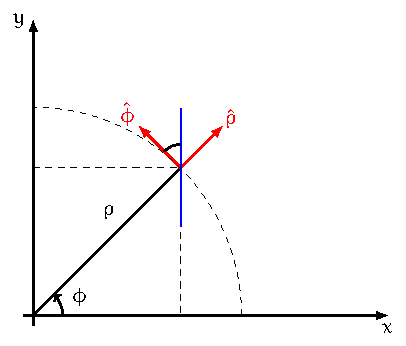
\includegraphics[width=10cm]{polar_coordinates.pdf}
	\begin{tikzpicture}
%		%Grid
%		\draw[thin, dotted] (0,0) grid (8,8);
%		\foreach \i in {1,...,8}
%		{
%			\node at (\i,-2ex) {\i};	
%		}
%		\foreach \i in {1,...,8}
%		{
%			\node at (-2ex,\i) {\i};	
%		}
%		\node at (-2ex,-2ex) {0};
		
		%Coordinates		
		\coordinate (A) at (6,0);
		\coordinate (B) at (0,0);
		\coordinate (C) at (2.5,2.5);
		\coordinate (B') at (2.5,3.5);
		\coordinate (A') at (1.8,3.2);
		
		%Axis
		\draw[thick,-latex] (-1ex,0) -- (6,0) node [below] {$x$};
		\draw[thick,-latex] (0,-1ex) -- (0,5) node [left] {$y$};
		
		%Vectors
		\draw[thick] (0,0) -- (2.5,2.5) node[pos=0.6, above left] {$\rho$};
		\draw[thick, red, -latex] (2.5,2.5) -- (3.2,3.2) node[pos=1.2] {$\hat{\rho}$};
		\draw[thick, red, -latex] (2.5,2.5) -- (1.8,3.2) node[pos=1.3] {$\hat{\phi}$};
		
		%Help Lines
		\draw[dashed] (0,2.5) -- (2.5,2.5) -- (2.5,0);
		\draw[blue, thick] (2.5,3.5) -- (2.5,1.5);
		\draw[dashed] (3.53,0) arc (0:90:3.53);
		
		%Angle
		\pic[draw, ->, thick, "$\phi$", angle eccentricity=1.7] {angle = A--B--C};
		\pic[draw, thick, angle radius=4mm, angle eccentricity=1.7] {angle = B'--C--A'};
		
	\end{tikzpicture}
\end{center}
We can also express the inputs to $ \vec{V} $ in polar coordinates, $(\rho,\phi)$.
\begin{align*}
  \vec{V}(\mathbf{r}) &= V_{\rho}\left(\rho,\phi\right)\hat{i} + V_{\phi}\left(\rho,\phi\right)\hat{j}.
\end{align*}
To extract the input functions, we take
\begin{align*}
  V_x &= \hat{i}\cdot \vec{V}\\
  V_y &= \hat{j}\cdot \vec{V}.
\end{align*}
Alternatively, we can project $ \vec{V} $ onto the $\hat\rho,\hat\phi$ axis:
\begin{align*}
  \vec{V}(\mathbf{r}) &= V_{\rho}\left(\rho,\phi\right)\hat{\rho} + V_{\phi}\left(\rho,\phi\right)\hat{\phi},
\end{align*}
and we extract
\begin{align*}
  V_{\rho} &= \hat{\rho}\cdot \vec{V}\\
  V_{\phi} &= \hat{\phi}\cdot \vec{V}.
\end{align*}
Notice that $\mathbf{r}$ is an abstract vector; we need to project it onto a basis.\newline

For instance, we can take the position vector and project it onto the cartesian and polar axes:
\begin{align*}
  \mathbf{s} &= x\hat{i} + y\hat{j}\\
             &= \rho \cos \phi \hat{i} + \rho \sin \phi \hat{j}\\
             &= \rho \hat{\rho}\\
             &= \sqrt{x^2 + y^2}\hat{\rho}
\end{align*}
The main reason we avoided using the $\hat\rho,\hat\phi$ axis up until this point is that $\rho$ and $\phi$ are \textit{position-dependent}, while the $\hat{i},\hat{j}$ axis is position-independent.\newline

Now, we must figure out the position-dependence of $\hat{\rho}$ and $\hat{\phi}$:
\begin{align*}
  d\mathbf{r} &= \pd{\mathbf{r}}{\rho}d\rho + \pd{\mathbf{r}}{\phi}d\phi.
\end{align*}
If we hold $\phi$ constant, it must be the case that any change in $\rho$ is in the $\hat\rho$ direction. Therefore,
\begin{align*}
  \hat\rho &= \frac{\pd{\mathbf{r}}{\rho}}{\left\Vert \pd{\mathbf{r}}{\rho} \right\Vert}\\
           &= \frac{\cos\phi\hat{i} + \sin\phi\hat{j}}{\left\vert \cos\phi\hat{i} + \sin\phi\hat{j} \right\vert}\\
           &= \cos\phi\hat{i} + \sin\phi\hat{j}.
\end{align*}
Similarly,
\begin{align*}
  \hat\phi &= \frac{\pd{\mathbf{r}}{\phi}}{\norm{\pd{\mathbf{r}}{\rho}}}\\
           &= \frac{-\rho\sin\phi\hat{i} + \rho\cos\phi\hat{j}}{\left\Vert -\rho\sin\phi\hat{i} + \rho\cos\phi\hat{j} \right\Vert}\\
           &= -\sin\phi\hat{i} + \cos\phi\hat{j}.
\end{align*}
Thus, we can see that the $\hat\rho,\hat,\phi$ axis is orthogonal. 
\begin{align*}
  \pd{\hat{\rho}}{\phi} &= -\sin\phi\hat{i} + \cos\phi\hat{j}\\
                        &= \hat{\phi},\\
  \pd{\hat{\phi}}{\phi} &= -\hat{\rho},\\
  \pd{\hat{\phi}}{\rho} &= 0,
  \intertext{and}
  \pd{\hat{\rho}}{\rho} &= 0
\end{align*}
\begin{example}[Velocity]
  \begin{align*}
    \mathbf{v} &= \frac{d \mathbf{s}}{dt}\\
               &= \frac{d}{dt}\left(x\hat{i}\right) + \frac{d}{dt}\left(y\hat{j}\right).
               \intertext{In the case of cartesian coordinates, $\hat{i}$ and $\hat{j}$ are constants.}
               &= v_{x}\hat{i} + v_{y}\hat{j}
  \end{align*}
  When we examine polar coordinates, since $\hat{\rho}$ and $\hat{\phi}$ are position-dependent, we must use the chain rule.\footnote{Note that $\hat{\rho} = \hat{\rho}\left(\rho,\phi\right)$ and $\hat{\phi} = \hat{\phi}(\rho,\phi)$.}
  \begin{align*}
    \mathbf{v} &= \frac{d\mathbf{s}}{dt}\\
               &= \frac{d\rho}{dt}\hat{\rho} + \rho \frac{d\hat{\rho}}{dt}\\
               &= \frac{d\rho}{dt}\hat{\rho} + \rho \left(\cancelto{0}{\pd{\hat{\rho}}{\rho}}\frac{d\rho}{dt} + \underbrace{\pd{\hat{\rho}}{\phi}}_{=\hat{\phi}}\frac{d\phi}{dt}\right)\\
               &= \frac{d\rho}{dt}\hat{\rho} + \rho \frac{d\phi}{dt}\hat{\phi}\\
               &= \dot\rho\hat\rho + \rho\dot\phi\hat\phi.
  \end{align*}
  Notice that $\dot\rho$ is the radial velocity and $\dot\phi = \omega$ is the angular velocity.
\end{example}
\subsubsection{Spherical and Cylindrical Coordinates}%
\begin{center}
  %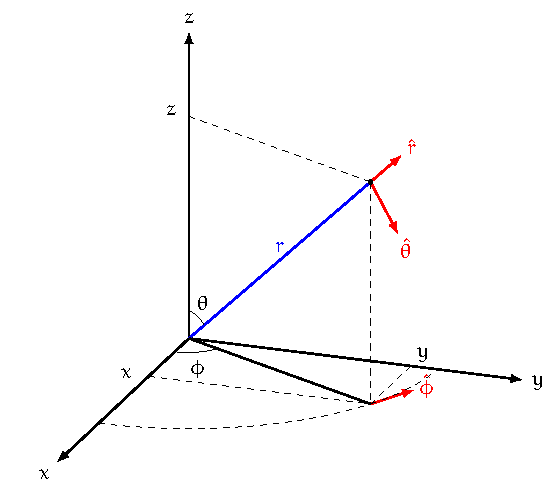
\includegraphics[width=10cm]{spherical_coordinates.pdf}

	\tdplotsetmaincoords{70}{110}
	%
	\pgfmathsetmacro{\thetavec}{48.17}
	\pgfmathsetmacro{\phivec}{63.5}
	%
	
	\begin{tikzpicture}[tdplot_main_coords]
		%Axis
		\draw[axis] (0,0,0) -- (6.5,0,0) node [pos=1.1] {$x$};
		\draw[axis] (0,0,0) -- (0,6,0) node [pos=1.05] {$y$};
		\draw[axis] (0,0,0) -- (0,0,5.5)  node [pos=1.05] {$z$};   
		
		%Unit Vectors
%		\tdplotsetcoord{p}{1}{90}{\phivec}
%    	\draw[univec] (2,4,0) -- ($(p)+(2,4,0)$) node [pos=1.35] {$\vu*{\varpi}$};
		\tdplotsetcoord{P'}{7}{\thetavec}{\phivec}
    	\draw[univec] (0,0,0) -- (P') node [pos=1.05] {$\hat{r}$};
    	\tdplotsetcoord{P''}{1}{90}{90+\phivec}
    	\draw[univec] (2,4,0) -- ($(P'') + (2,4,0)$) node [pos=1.3] {$\hat{\phi}$};
    	\tdplotsetcoord{P'''}{1}{90+\thetavec}{\phivec}
    	\draw[univec] (2,4,4) -- ($(P''') + (2,4,4)$) node [pos=1.3] {$\hat{\theta}$};
		
		%Vectors
		\tdplotsetcoord{P}{6}{\thetavec}{\phivec}
		\draw[vec] (0,0,0) -- (P) node [midway, above] {$r$};
		\draw[thick] (0,0,0) -- (2,4,0);
		
		%Help Lines
		\draw[dashed] (2,4,4) -- (2,4,0);
		\draw[dashed] (2,0,0) -- (2,4,0) node [pos=-0.1] {$x$};
		\draw[dashed] (0,4,0) -- (2,4,0) node [pos=-0.3] {$y$};
		\draw[dashed] (0,0,4) -- (2,4,4) node [pos=-0.1] {$z$};
		\draw[dashed, tdplot_main_coords] (4.47,0,0) arc (0:90:4.47);
		
		%Point
		\node[fill=black, circle, inner sep=0.8pt] at (2,4,4) {};
		
		%Angles
		\tdplotdrawarc{(0,0,0)}{0.7}{0}{\phivec}{below}{$\phi$}
		 
	    \tdplotsetthetaplanecoords{\phivec}
	    \tdplotdrawarc[tdplot_rotated_coords]{(0,0,0)}{0.5}{0}{\thetavec}{}{}
	    \node at (0,0.25,0.67) {$\theta$};
		
	\end{tikzpicture}
\end{center}
\begin{center}
  	\tdplotsetmaincoords{70}{110}
	%
	\pgfmathsetmacro{\thetavec}{48.17}
	\pgfmathsetmacro{\phivec}{63.5}
	%
	
	\begin{tikzpicture}[tdplot_main_coords]
		%Axis
		\draw[axis] (0,0,0) -- (6,0,0) node [pos=1.1] {$x$};
		\draw[axis] (0,0,0) -- (0,6,0) node [pos=1.05] {$y$};
		\draw[axis] (0,0,0) -- (0,0,5.5)  node [pos=1.05] {$z$};   
		
		%Help Lines
		\draw[dashed] (2,4,4) -- (2,4,0);
		\draw[dashed] (2,0,0) -- (2,4,0) node [pos=-0.1] {$x$};
		\draw[dashed] (0,4,0) -- (2,4,0) node [pos=-0.35, left] {$y$};
		\draw[dashed] (0,0,4) -- (2,4,4) node [pos=-0.1] {$z$};
		\draw[dashed, tdplot_main_coords] (4.47,0,0) arc (0:90:4.47);
		
		%Unit Vectors
		\tdplotsetcoord{P'}{1}{90}{\phivec}
    	\draw[univec] (2,4,0) -- ($(P')+(2,4,0)$) node [pos=1.3] {$\hat{\rho}$};
    	\tdplotsetcoord{P''}{1}{90}{90+\phivec}
    	\draw[univec] (2,4,0) -- ($(P'') + (2,4,0)$) node [pos=1.3] {$\hat{\phi}$};
    	
    	%Vectors
		\tdplotsetcoord{P}{6}{\thetavec}{\phivec}
		\draw[vec] (0,0,0) -- (P);
		\draw[thick] (0,0,0) -- (2,4,0) node [pos=0.6, above] {$\rho$};
		
		%Point
		\node[fill=black, circle, inner sep=0.8pt] at (2,4,4) {};
		
		%Angles
		\tdplotdrawarc{(0,0,0)}{0.7}{0}{\phivec}{below}{$\phi$}
		
	\end{tikzpicture}
\end{center}
\begin{table}
  \centering
  \renewcommand{\arraystretch}{1.5}
  \begin{tabular}{c|c|c}
    Polar & Cylindrical & Spherical\\
    \hline\hline
    $\mathbf{s} = s(\rho,\phi)$ & $\mathbf{s} = s(\rho,\phi,z)$ & $\mathbf{s} = s(r,\phi,\theta)$\\
    $\mathbf{s} = \rho\cos\phi\hat{i} + \rho\sin\phi\hat{j}$ & $\mathbf{s} = \rho\cos\phi\hat{i} + \rho\sin\phi\hat{j} + z\hat{k}$ & $\mathbf{s} = r\cos\phi\sin\theta\hat{i} + r\sin\phi\sin\theta\hat{j} + r\cos\theta\hat{k}$
  \end{tabular}
  \caption{Coordinate Conversions}
\end{table}
%\begin{center}
%  \renewcommand{\arraystretch}{1.5}
%  \begin{tabular}{c|c|c}
%    Polar & Cylindrical & Spherical\\
%    \hline\hline
%    $\mathbf{s} = s(\rho,\phi)$ & $\mathbf{s} = s(\rho,\phi,z)$ & $\mathbf{s} = s(r,\phi,\theta)$\\
%    $\mathbf{s} = \begin{pmatrix}\rho\cos\phi\\\rho\sin\phi\end{pmatrix}$ & $\mathbf{s} = \begin{pmatrix}\rho\cos\phi\\\rho\sin\phi\\z\end{pmatrix}$ & $\mathbf{s} = \begin{pmatrix}r\cos\phi\sin\theta\\r\sin\phi\sin\theta \\ r\cos\theta\end{pmatrix}$
%  \end{tabular}
%\end{center}
Here,\footnote{Physicists amirite?} $\phi$ denotes the polar angle and $\theta$ denotes the azimuthal angle. Notice that $\phi \in [0,2\pi)$ and $\theta \in [0,\pi]$.\newline

We can see that $\hat\rho$, $\hat\phi$, and $\hat\theta$ in spherical coordinates are also position-dependent.
\begin{align*}
  \hat r &= \frac{\pd{\mathbf{s}}{r}}{\norm{\pd{\mathbf{s}}{r}}}\\
         &= \sin\theta\cos\phi\hat{i} + \sin\theta\sin\phi\hat{j} + \cos\theta\hat{k}\\
  \hat{\phi} &= \frac{\pd{\mathbf{s}}{\phi}}{\norm{\pd{\mathbf{s}}{\phi}}}\\
             &= -\sin\phi\hat{i} + \cos\phi\hat{j}\\
  \hat{\theta} &= \frac{\pd{\mathbf{s}}{\theta}}{\norm{\pd{\mathbf{s}}{\theta}}}\\
               &= \cos\phi\cos\theta\hat{i} + \cos\theta\sin\phi\hat{j} - \sin\theta\hat{k}
\end{align*}
\subsubsection{Scale Factors and Jacobians}%
\begin{table}
  \centering
  \renewcommand{\arraystretch}{1.5}
  \begin{tabular}{c|c|c|c}
    Coordinate System & Line Element & Area Element & Volume Element\\
    \hline\hline
    Polar & $d \mathbf{s} = \hat\rho d\rho + \rho \hat\phi d\phi$ & $d\mathbf{a} = r\:drd\phi$ & ---\\
    Cylindrical & $d \mathbf{s} = \hat\rho d\rho + \rho\hat\phi d\phi + \hat k dz$ & $d\mathbf{a} = \hat{\rho}\:\rho d\phi dz$ & $d\tau = r\:dr d\phi dz$\\
    Spherical & $d \mathbf{s} = \hat r dr + r\sin\theta \hat\phi d\phi + r\hat\theta d\theta$ &  $d \mathbf{a} = \hat{r}\:r^2\sin\theta d\phi d\theta$ & $d\tau = r^2\sin\theta\:dr d\phi d\theta$
  \end{tabular}
  \caption{Line, Area, and Volume Elements in Different Coordinate Systems}
\end{table}
In cylindrical coordinates, we can use the chain rule to find the value of $d \mathbf{r}$:
\begin{align*}
  d \mathbf{r} &= \hat{\rho}d\rho + \rho\hat\phi d\phi + \hat k dz.
\end{align*}
The extra factor of $\rho$ in the expression of $\rho\hat\phi d\phi$ is the \textit{scale factor} on $\phi$.\newline

Similarly, in spherical coordinates, we have
\begin{align*}
  d \mathbf{r} &= \hat{r} dr +  r\sin\theta \hat{\phi}d\phi + r\hat{\theta}d\theta,
\end{align*}
with scale factors of $r\sin\theta$ on $\hat\phi d\phi$ and $r$ on $\hat\theta d\theta$.\newline

When we go from line elements (of the form $d\mathbf{r}$) to area elements (of the form $d \mathbf{a}$), we can see that the area element in polar coordinates is $d \mathbf{a} = \rho d\rho d\phi$ --- we need the extra factor of $\rho$ to account for the fact that the magnitude of the area element scales with the radius.\newline

Similarly, the volume element in cylindrical coordinates is $d\tau = r dr d\phi dz$ and the volume element in spherical coordinates is $r^2 \sin \theta dr d\phi d\theta$.\newline

Recall that the definition of an angle $\phi$ that subtends an arc length $s$ is $\phi \frac{s}{r}$, where $r$ is the radius of a circle. We can imagine a similar concept on a sphere --- a \textit{solid angle} measured in steradians is of the form $\Omega = \frac{A}{r^2}$, where $A$ denotes the surface area subtended by the angle $\Omega$. In particular, since $d\Omega = \frac{dA}{r^2}$, we find that $d\Omega = \sin\theta d\phi d\theta$.\newline

When we are dealing with products of scale factors, we need to use the Jacobian to determine the proper scale factor on any given element:
\begin{align*}
  d\mathbf{a} &= dx dy\\
              &= \left\vert J \right\vert \:du dv,
\end{align*}
where $|J|$ denotes the determinant of the Jacobian matrix. We write the Jacobian as follows:
\begin{align*}
  J &= \frac{\partial \left(x,y\right)}{\partial \left(u,v\right)}\\
    &= \begin{pmatrix}\pd{x}{u} & \pd{y}{u}\\ \pd{x}{v} & \pd{y}{v}\end{pmatrix}.
\end{align*}
We specifically desire the determinant:
\begin{align*}
  |J| &= \pd{x}{u}\pd{y}{v} - \pd{y}{u}\pd{x}{v}.
\end{align*}
\subsection{Complex Numbers}%
\begin{table}
  \centering
  \renewcommand{\arraystretch}{1.75}
  \begin{tabular}{c|c}
    Quantity & Expression and/or Criterion\\
    \hline\hline
    Cartesian form & $z = a + bi$\\
    Polar form & $z = re^{i\phi}$\\
    $r$ & $\sqrt{a^2 + b^2}$\\
    $\phi$ & $\arg z = \arctan\left(\frac{b}{a}\right)$\\
    \hline
    Cartesian $\overline{z}$ & $\overline{z} = a-bi$\\
    Polar $\overline{z}$ & $\overline{z} = re^{-i\phi}$\\
    $|z|$ & $\sqrt{z\overline{z}}$\\
    \hline
    $\re(z)$ & $\re(z) = \frac{z + \overline{z}}{2}$\\
    $\im(z)$ & $\im(z) = \frac{z - \overline{z}}{2i}$\\
    $\cos\phi$ & $\frac{e^{i\phi} + e^{-i\phi}}{2}$\\
    $\sin\phi$ & $\frac{e^{i\phi} - e^{-i\phi}}{2i}$\\
    \hline
    $e^{i\phi}$ & $\cos \phi + i\sin\phi$\\
    $e^{in\phi}$ & $\cos \left(n\phi\right) + i\sin \left(n\phi\right)$
  \end{tabular}
  \caption{Complex Number Identities}
\end{table}
\subsubsection{Introduction}%

\begin{center}
  \begin{tikzpicture}[scale = 2]
  \def\xmax{2.0}
  \def\ymax{1.6}
  \def\R{1.9}
  \def\ang{35}
  \coordinate (O) at (0,0);
  \coordinate (R) at (\ang:\R);
  \coordinate (-R) at (-\ang:\R);
  \coordinate (X) at ({\R*cos(\ang)},0);
  \coordinate (Y) at (0,{\R*sin(\ang)});
  \coordinate (-Y) at (0,{-\R*sin(\ang)});
  \node[fill=mydarkblue,circle,inner sep=0.8] (R') at (R) {};
  \node[fill=mydarkred,circle,inner sep=0.8] (-R') at (-R) {};
  \node[mydarkblue,above right=-2] at (R') {$z=a+bi=re^{i\phi}$};
  \node[mydarkred,below right=-1] at (-R') {$\overline{z}=a-bi=re^{-i\phi}$};
  \draw[dashed,mydarkblue]
    (Y) -- (R') --++ (0,{0.1-\R*sin(\ang)});
  \draw[dashed,mydarkred]
    (-Y) -- (-R') --++ (0,{\R*sin(\ang)-0.45});
  \draw[->,line width=0.9] (-0.65*\xmax,0) -- (\xmax+0.05,0) node[right] {Re};
  \draw[->,line width=0.9] (0,-\ymax) -- (0,\ymax+0.05) node[left] {Im};
  \draw[vector] (O) -- (R') node[pos=0.55,above left=-2] {$r$};
  \draw[vector,myred] (O) -- (-R') node[pos=0.55,below left=-2] {$r$};
  \draw pic[->,"$\phi$",mydarkblue,draw=mydarkblue,angle radius=23,angle eccentricity=1.24]
    {angle = X--O--R};
  \draw pic[<-,"$-\phi$"{right=-1},mydarkred,draw=mydarkred,angle radius=20,angle eccentricity=1]
    {angle = -R--O--X};
  %\tick{X}{90} node[scale=0.9,left=6,below right=-2] {$x = r\cos\theta$};
  \tick{X}{90} node[scale=1,below=-1] {$x$};
  \tick{Y}{ 0} node[mydarkblue,scale=1,left] {$y$}; %r\sin\theta = 
  \tick{-Y}{ 0} node[mydarkred,scale=1,left] {$-y$};
\end{tikzpicture}
\end{center}
A complex number is denoted
\begin{align*}
  z &= a + bi
\end{align*}
where $i^2 = -1$ and $a,b\in \R$. This is known as the Cartesian representation. However, we can also imagine $z$ as the polar representation:
\begin{align*}
  z &= re^{i\phi},
\end{align*}
where $\phi = \arg z$ is known as the argument, and $r = |z|$ is the modulus. We can see the relation between the Cartesian and polar representations through Euler's identity:\footnote{This can be proven relatively easily through substitution into the Taylor series, which is allowed because $e^z$ is entire.}
\begin{align*}
  r\left(\cos \phi + i\sin\phi\right) &= re^{i\phi}.
\end{align*}
We denote the conjugate of $z$ as $\overline{z}$, found by $\overline{z} = a - bi = re^{-i\phi}$.\newline

We find $\re(z)$ and $\im(z)$, the real and imaginary parts of $z$, by
\begin{align*}
  \re(z) &= \frac{z + \overline{z}}{2}\\
  \im(z) &= \frac{z - \overline{z}}{2i}.
\end{align*}
We say that a complex number of the form $e^{i\phi}$ is a \textit{pure phase}, as $\left\vert e^{i\phi} \right\vert = 1$.\newline

To find if some complex number $z$ is purely real or purely imaginary, we can use the following criterion:
\begin{align*}
  z\in \R \Leftrightarrow z = \overline{z}\\
  z\in i\R \Leftrightarrow z = -\overline{z}.
\end{align*}
\begin{example}[Real, Imaginary, or Complex?]
  Consider
  \begin{align*}
    z_1 &= i^{i}.
  \end{align*}
  To find if this is purely real or complex, we take
  \begin{align*}
    \overline{z_1} &= \left(-i\right)^{-i}\\
               &= \left(\frac{1}{-i}\right)^{i}\\
               &= i^{i}.
  \end{align*}
  Thus, $z_1\in \R$. In order to determine the value of $i^i$, we substitute the polar form:
  \begin{align*}
    z_1 &= \left(e^{i\frac{\pi}{2}}\right)^{i}\\
        &= e^{-\frac{\pi}{2}}.
  \end{align*}
\end{example}
\subsubsection{Some Trigonometry with Complex Exponentials}%
Consider $z = \cos \phi + i\sin\phi$. We can see that
\begin{align*}
  \re(z) &= \cos\phi\\
         &= \frac{\left(\cos \phi + i\sin\phi\right) + \left(\cos\phi - i\sin\phi\right)}{2}\\
         &= \frac{e^{i\phi} + e^{-i\phi}}{2}\\
  \im(z) &= \sin\phi\\
         &= \frac{\left(\cos\phi + i\sin\phi\right) - \left(\cos\phi - i\sin\phi\right)}{2i}\\
         &= \frac{e^{i\phi} - e^{-i\phi}}{2i}.
\end{align*}
We can actually define $\sin\phi$ and $\cos\phi$ with the above derivation.\newline

\begin{theorem}[De Moivre]
\begin{align*}
  e^{inx} &= \cos\left(nx\right) + i\sin \left(nx\right)\\
          &= \left(e^{ix}\right)^{n}\\
          &= \left(\cos x + i\sin x\right)^n.
\end{align*}
\end{theorem}
\begin{example}[Finding $\cos \left(2x\right)$ and $\sin \left(2x\right)$]
  \begin{align*}
    \cos\left(2x\right) + i\sin \left(2x\right) &= \left(\cos x + i\sin x\right)^2\\
                                                &= \left(\cos^2 x - \sin^2 x\right) + i\left(2\sin x \cos x\right).
  \end{align*}
  Since the real parts and imaginary parts have to be equal, this means
  \begin{align*}
    \cos 2x &= \cos^2 x - \sin^2 x\\
    \sin^2 x &= 2\sin x \cos x.
  \end{align*}
\end{example}
In particular, we can see that $e^{in\phi} = \left(-1\right)^n$ and $e^{in\frac{\pi}{2}} = i^n$.\footnote{This will be especially useful when we get to Fourier series.}\newline

Additionally, we can see that for $z = re^{i\phi}$,
\begin{align*}
  z^{1/m} &= \left(re^{i\phi + 2\pi n}\right)^{1/m}\\
          &= r^{1/m}e^{i\frac{1}{m}\left(\phi + 2\pi n\right)},
\end{align*}
where $n\in \N$ and $m$ is fixed. For $r = 1$, we call these values the $m$ roots of unity.
\begin{example}[Waves and Oscillations]
  Recall that for a wave with spatial frequency $k$, angular frequency $\omega$, and amplitude $A$, the wave is represented by
  \begin{align*}
    f(x,t) &= A\cos\left(kx - \omega t\right).
  \end{align*}
  The speed of a wave $v$ is equal to $\frac{\omega}{k}$.\newline

  Simple harmonic motion is characterized by the solution to the differential equation $\ddot{\mathbf{x}} = -\omega^2 \mathbf{x}$, where $\mathbf{x}$ denotes position. In simple harmonic motion, there is no spatial motion, meaning our function is only of time:
  \begin{align*}
    f(t) &= A\cos \omega t\\
         &= \re\left(Ae^{i\omega t}\right).
  \end{align*}
  As a result of the representation of complex numbers in polar form, we can do math entirely in exponentials, then take the real part of our solution to find $f(t)$.\newline

  Unfortunately, in the real world, there is friction; as a result, our oscillation is damped by an exponential factor.
\end{example}
\begin{example}[Hyperbolic Sine and Hyperbolic Cosine]
  We wish to calculate $\cos ix$ and $\sin ix$.
  \begin{align*}
    \cos ix &= \frac{1}{2}\left(e^{i\left(ix\right)} + e^{-i\left(ix\right)}\right)\\
            &= \frac{e^{-x} + e^{x}}{2}
  \end{align*}
  We define $\cosh x = \cos \left(ix\right)$. Additionally,
  \begin{align*}
    - i\sin ix &= -i\frac{1}{2i}\left(e^{i\left(ix\right)} - e^{-i\left(ix\right)}\right)\\
            &= i\frac{e^{x} - e^{-x}}{2i}.\\
            &= \frac{e^{x} - e^{-x}}{2}.
  \end{align*}
  We define $\sinh x = -i\sin\left(ix\right)$.\newline

  Similar to how $\cos^2 x + \sin^2 x = 1$, we can find that $\cosh^2 x - \sinh^2 x = 1$.
\end{example}
\subsection{Index Algebra}%
We usually denote vectors by either $\vec{A}$, $\mathbf{A}$, or
\begin{align*}
  \begin{pmatrix}a_1\\a_2\\\vdots\\a_n\end{pmatrix},
\end{align*}
which is defined by a basis.\newline

If we imagine we are in $n$-dimensional space, we can let $A_i$ where $i = 1,2,\dots,n$ denote both
\begin{itemize}
  \item the $i$th component of $\vec A$;
  \item the entire vector $\vec{A}$ (since $i$ can be arbitrary).
\end{itemize}
\subsubsection{Contractions and Dummy Indices}%
Consider $C = AB$, where $A,B $ are $n\times m$ and $m\times p$ matrices respectively.
\begin{align*}
  C &= \begin{pmatrix}A_{11} & A_{12} & \cdots & A_{1m}\\
  \vdots & \vdots & \ddots & \vdots\\
A_{n1} & A_{n2} & \cdots & A_{nm}\end{pmatrix} \begin{pmatrix}B_{11} & B_{12} & \cdots & B_{1p}\\
  \vdots & \vdots & \ddots & \vdots\\
B_{m1} & B_{m2} & \cdots & B_{mp}\end{pmatrix}.
\end{align*}
%The index notation description of this multiplication is much more contracted than the traditional method learned in linear algebra:
%\begin{align*}
%  C_{ij} &= \sum_{k=1}^{n} A_{ik}B_{kj}.
%\end{align*}
%This might seem like a very convoluted system for small matrices.\newline
%
%However, looking at $AB$ compared to $BA$, we see that
%\begin{align*}
%  \left(AB\right)_{ij} &= \sum_{k} A_{ik}B_{kj}\\
%                       &= \sum_{k}B_{kj}A_{ik},\\
%  \left(BA\right)_{ij} &= \sum_{k}B_{ik}A_{kj}\\
%                       &= \sum_{k}A_{kj}B_{ik}.
%\end{align*}
\begin{definition}[Matrix Multiplication in Index Notation]
  For matrices $A$ and $B$, where $A$ is an $m\times n$ and $B$ is a $n\times p$ matrix, we write
  \begin{align*}
    C_{ij} &= \sum_{k=1}^{n}A_{ik}B_{kj}
  \end{align*}
\end{definition}
We say that $k$ is a dummy index, since $k$ takes values from $1$ to $n$. Note that the value we calculate is $C_{ij}$; in other words, in the sum $\sum_{k}A_{ik}B_{kj}$, the indices of the form $ij$ are the ``net indices'' from the multiplication.\newline

Note that if $C = BA$, then
\begin{align*}
  C_{ij} &= \sum_{k=1}^{n}B_{ik}A_{kj}\\
         &= \sum_{k=1}^{n}A_{kj}B_{ik}\\
         &\neq \sum_{k=1}^{n}A_{ik}B_{kj}.
\end{align*}
The corresponding fact is that $AB\neq BA$ necessarily.\newline

Note that the index that is summed over always appears exactly twice.
\begin{definition}[Symmetric Matrix]
  Let $C$ be a matrix. Then, we say $C$ is symmetric if
  \begin{align*}
    C_{ij} &= C_{ji}
  \end{align*}
\end{definition}
\begin{definition}[Antisymmetric Matrix]
  Let $C$ be a matrix. We say $C$ is antisymmetric if
  \begin{align*}
    C_{ij} &= -C_{ji}.
  \end{align*}
\end{definition}
We can always decompose a random matrix into the sum of a symmetric matrix and an antisymmetric matrix.
\subsubsection{Two Special Tensors}%
\begin{table}
  \centering
  \renewcommand{\arraystretch}{1.75}
  \begin{tabular}{c|c|c}
    Name & Notation & Definition\\
    \hline\hline
    Kronecker Delta & $\delta_{ij}$ &$\delta_{ij} = \begin{cases}1 & i=j\\ 0 & i\neq j \end{cases}$\\
    Levi--Civita Symbol & $\epsilon_{ijk}$ & $\epsilon_{ijk} = \begin{cases}1 & \text{$(i,j,k) = (1,2,3)$ cyclically}\\-1 & \text{$(i,j,k) = (2,1,3)$ cyclically}\\0 & \text{else} \end{cases}$
  \end{tabular}
  \caption{$\delta_{ij}$ and $\epsilon_{ijk}$}
\end{table}
\begin{table}
  \centering
  \renewcommand{\arraystretch}{1.25}
  \begin{tabular}{c|c}
    Order of $\left(i,j,k\right)$ & Value of $\epsilon_{ijk}$\\
    \hline\hline
    $1,2,3$ & $1$\\
    $3,1,2$ & $1$\\
    $2,3,1$ & $1$\\
    \hline
    $1,3,2$ & $-1$\\
    $2,1,3$ & $-1$\\
    $3,2,1$ & $-1$\\
    \hline
    else & $0$
  \end{tabular}
  \caption{Values of $\epsilon_{ijk}$}
\end{table}
\begin{table}
  \centering
  \renewcommand{\arraystretch}{1.5}
  \begin{tabular}{c|c}
    Value & Index Notation\\
    \hline\hline
    $\mathbf{A}\times \mathbf{B}$ & $\displaystyle\sum_{i,j,k}\epsilon_{ijk}A_iB_j\hat{e}_k$\\
    $\left(\mathbf{A}\times \mathbf{B}\right)_{\ell}$  & $\displaystyle\sum_{i,j}\epsilon_{ij\ell}A_iB_j$\\
    $\left(\hat{e}_i \times \hat{e}_j\right)\cdot \hat{e}_{k}$ & $\epsilon_{ijk}$\\
    \hline
    $B_i$ & $\displaystyle\sum_{\alpha}B_{\alpha}\delta_{\alpha i}$\\
    $\mathbf{A}\cdot \mathbf{B}$ & $\displaystyle\sum_{i,j}A_iB_j\delta_{ij}$\\
    \hline
    $\displaystyle\sum_{j,k}\epsilon_{mjk}\epsilon_{njk}$ & $2\delta_{mn}$\\
    $\displaystyle\sum_{\ell}\epsilon_{mn\ell}\epsilon_{ij\ell}$ & $\delta_{mi}\delta_{nj} - \delta_{mj}\delta_{ni}$
  \end{tabular}
  \caption{Vector Identities, $\epsilon_{ijk}$, and $\delta_{ij}$}
\end{table}
\begin{definition}[Kronecker Delta]
  The Kronecker Delta, $\delta_{ij}$, is the tensor that denotes the identity matrix.
  \begin{align*}
    \delta_{ij} &= \begin{cases}
      1 & i=j\\
      0 & i\neq j
    \end{cases}
  \end{align*}
\end{definition}
\begin{example}[Extracting an Index]
  Consider $A$ as vector. Then,
  \begin{align*}
    \sum_{i}A_i \delta_{ij} &= A_j.
  \end{align*}
  In other words, the Kronecker Delta collapses the sum to the $j$th index.
\end{example}
\begin{example}[Orthonormal Basis from Kronecker Delta]
  Let $\set{\hat{e}_i}_{i=1}^{n}$ be a basis for some vector space $V$. If
  \begin{align*}
    \hat{e}_i\cdot \hat{e}_j &= \delta_{ij}
  \end{align*}
  for every $i,j$, then $\set{\hat{e}_i}_{i=1}^{n}$ is an orthonormal basis for $V$.
\end{example}
\begin{definition}[Levi--Civita Symbol]
  In two dimensions, as a matrix, we write
  \begin{align*}
    \epsilon_{ij} &= \begin{pmatrix}0 & 1 \\ -1 & 0\end{pmatrix},
  \end{align*}
  meaning
  \begin{align*}
    \epsilon_{ij} &= \begin{cases}
      1 & i=1,j=2\\
      -1 & i=2,j=1\\
      0 & \text{else}
    \end{cases}.
  \end{align*}
  The Levi--Civita Symbol is antisymmetric, just as the Kronecker Delta is symmetric.\newline

  In three dimensions, we define
  \begin{align*}
    \epsilon_{ijk}  &= \begin{cases}
      1 & \text{$\left(i,j,k\right) = \left(1,2,3\right)$ cyclically}\\
      -1 & \text{$\left(i,j,k\right) = \left(2,1,3\right)$ cyclically}\\
      0 & \text{else}
    \end{cases}.
  \end{align*}
  In other words, $\epsilon_{ijk} = -\epsilon_{jik}$.
\end{definition}
\begin{exercise}[Relations between $\delta_{ij}$ and $\epsilon_{ijk}$]
  \begin{align*}
    \sum_{j,k}\epsilon_{mjk}\epsilon_{njk} &= 2\delta_{mn}\\
    \sum_{\ell}\epsilon_{mn\ell}\epsilon_{ijl} &= \delta_{mi}\delta_{nj} - \delta_{mj}\delta_{ni}
  \end{align*}
\end{exercise}
\begin{definition}[Dot Product]
  Let $\set{\hat{e}_i}_{i=1}^{n}$ be an orthonormal basis for $V$. Let $\mathbf{A} = \sum_{i}A_i\hat{e}_i$ and $\mathbf{B} = \sum_{i}B_i\hat{e}_i$. Then,
  \begin{align*}
    \mathbf{A}\cdot \mathbf{B} &= \sum_{i,j}\left(A_i\hat{e}_i\right)\cdot\left(B_j\hat{e}_j\right)\\
                               &= \sum_{i,j}A_iB_j \left(\hat{e}_i \cdot \hat{e}_j\right)\\
                               &= \sum_{i,j}A_iB_j \delta_{ij}\\
                               &= \sum_{i}A_iB_i
  \end{align*}
\end{definition}
\begin{definition}[Cross Product]
  Let $\set{\hat{e}_i}_{i=1}^{3}$ be the standard basis over $\R^3$. Let $\mathbf{A} = \sum_{i}A_i\hat{e}_i$ and $\mathbf{B} = \sum_{i}B_i\hat{e}_i$. Then,
  \begin{align*}
    \mathbf{A}\times \mathbf{B} &= \sum_{i,j}\left(A_i\hat{e}_i\right)\times \left(B_j\hat{e}_j\right)\\
                                &= \sum_{i,j}A_iB_j \left(\hat{e}_i \times \hat{e}_j\right)\\
                                &= \sum_{i,j,k}A_iB_j\left(\epsilon_{ijk}\hat{e}_k\right).
  \end{align*}
  Instead of asking about $\mathbf{A}\times \mathbf{B}$, we ask about $\left(\mathbf{A}\times \mathbf{B}\right)_{\ell}$, yielding
  \begin{align*}
    \left(\mathbf{A}\times \mathbf{B}\right)_{\ell} &= \left(\mathbf{A}\times \mathbf{B}\right)\cdot \hat{e}_{\ell}\\
                                                    &= \left(\sum_{i,j,k}A_iB_j\left(\epsilon_{ijk}\hat{e}_k\right)\right)\cdot \hat{e}_{\ell}\\
                                                    &= \sum_{i,j}\epsilon_{ij\ell}A_iB_j.
  \end{align*}
\end{definition}
\begin{remark}
  This notation for $\mathbf{A}\times \mathbf{B}$ automatically shows us that
  \begin{align*}
    \left(\mathbf{B}\times \mathbf{A}\right)_{\ell} &= \sum_{i,j}\epsilon_{ij\ell}B_iA_j\\
                                                    &= -\sum_{i,j}\epsilon_{ji\ell}B_iA_j\\
                                                    &= -\sum_{i,j}\epsilon_{ji\ell}A_jB_i\\
                                                    &= -\sum_{i,j}\epsilon_{ij\ell}A_iB_j\tag*{$i,j$ are dummy indices}\\
                                                    &= -\left(\mathbf{A}\times \mathbf{B}\right)_{\ell}.
  \end{align*}
\end{remark}
\begin{example}[Central Force and Angular Momentum]
  A central force is defined by
  \begin{align*}
    \mathbf{F} &= f(r)\hat{r},
  \end{align*}
  where $\hat{r}$ is a radial vector.\newline

  Angular momentum is defined by
  \begin{align*}
    \mathbf{L} &= \mathbf{r}\times \mathbf{p},
  \end{align*}
  where $\mathbf{r}$ denotes position and $\mathbf{p}$ denotes momentum. Then,
  \begin{align*}
    \frac{d\mathbf{L}}{dt} &= \frac{d}{dt}\left(\mathbf{r}\times \mathbf{p}\right)\\
                           &= \left(\frac{d}{dt}\mathbf{r}\times \mathbf{p}\right) + \mathbf{r}\times \left(\frac{d\mathbf{p}}{dt}\right)\\
                           &= m\left(\frac{d}{dt}\mathbf{r}\times \frac{d}{dt}\mathbf{r}\right) + \mathbf{r}\times \left(f(r)\hat{r}\right)\\
                           &= f(r)\left(\mathbf{r}\times \hat{r}\right).
  \end{align*}
  This implies that $\frac{d\mathbf{L}}{dt} = 0$ under a central force.
\end{example}
\begin{example}[Determinant]
  Let $\mathbf{M} = M_{ij}$ be square. We denote $\mathbf{M}_i$ to be the vector denoting the $i$th-row. Then,
  \begin{align*}
    m &= \left\vert \mathbf{M} \right\vert\\
      &= \mathbf{M}_1\cdot \left(\mathbf{M}_2 \times \mathbf{M}_3\right)\\
      &= \mathbf{M}_3 \cdot \left(\mathbf{M}_1\times \mathbf{M}_2\right)\\
      &= \mathbf{M}_2 \cdot \left(\mathbf{M}_3\times \mathbf{M}_1\right).
  \end{align*}
\end{example}
\begin{example}[Trace]
  Let $\mathbf{M} = M_{ij}$ be a square matrix. We define $\tr\left(\mathbf{M}\right) = \sum_{i}M_{ii}$. Equivalently,
  \begin{align*}
    \tr\left(\mathbf{M}\right) &= \sum_{ij}M_{ij}\delta_{ij}\\
                                     &= \sum_{i}M_{ii}.
  \end{align*}
  Note that
  \begin{align*}
    \tr\left(I_{n}\right) &= \sum_{i}\delta_{ii}\\
                                     &= n.
  \end{align*}
  When we upgrade to $3$ matrices, we take
  \begin{align*}
    \tr\left(ABC\right) &= \sum_{i,j}\left(\sum_{k,\ell}A_{ik}B_{k\ell}C_{\ell j}\right)\delta_{ij}\\
                        &= \sum_{i,k,\ell}A_{ik}B_{k\ell}C_{\ell i}\\
                        &= \sum_{i,k,\ell}C_{\ell i}A_{ik}B_{k\ell}\\
                        &= \tr\left(CAB\right).
  \end{align*}
  In other words, the trace is invariant under cyclic permutations.
\end{example}
\begin{example}[Moment of Inertia Tensor]\hfill
%  \begin{center}
%    \begin{tikzpicture}
%  \def\R{3.3}   % circle radius
%  \def\r{1.4}   % mass radius (inner sep)
%  \def\L{1.2}   % angular momentum
%  \def\v{0.8}   % velocity
%  \def\l{0.35}  % angular momentum
%  \def\ang{18}  % mass angular position
%  \def\angp{40} % angle to feign perspective
%  \coordinate (O) at (\ang+90+\angp:0.4*\R);
%  \coordinate (R1) at (\ang-180:0.8*\R);
%  \coordinate (R2) at (0,0);
%  \coordinate (R3) at (\ang:0.65*\R);
%  \coordinate (R1E) at ($(O)!1.25!(R1)$); % R1 extended
%  \draw[Lvec] (O) --++ (0,\L) node[below right=0] {$\vb{L}$};
%  \draw[xcol!80!black] (\ang-180:\R) -- (\ang:\R);
%  \draw[dashed] (R1) -- (R1E);
%  \draw[pvec] (R1) --++ (\ang:\v) node[below=1] {$\vb{p}$};
%  \draw[pvec] (R2) --++ (\ang:\v) node[below=1] {$\vb{p}$};
%  \draw[pvec] (R3) --++ (\ang:\v) node[below=1] {$\vb{p}$};
%  \node[mass,circle,inner sep=2] (R1') at (R1) {};
%  \node[mass,circle,inner sep=2] (R2') at (R2) {};
%  \node[mass,circle,inner sep=2] (R3') at (R3) {};
%  \draw[rvec] (O) -- (R1') node[midway,above left=-2] {$\vb{r}$};
%  \draw[rvec] (O) -- (R2') node[midway,below left=-3] {$\vb{r}_\mathrm{t}$};
%  \draw[rvec] (O) -- (R3') node[midway,above=-1] {$\vb{r}$};
%  \draw (R2)++(\ang-180:\l) --++ (\ang+90+\angp:\l) --++ (\ang:\l);
%  %\draw pic["$\theta$",draw,angle radius=24,angle eccentricity=1.24] {angle=R2--R1--O};
%  \draw pic["$\theta$",draw,angle radius=7,angle eccentricity=1.5] {angle=R1E--R1--R2};
%\end{tikzpicture}
%  \end{center}
  Recall that
  \begin{align*}
    \mathbf{L} &= \mathbf{r}\times \mathbf{p},\\
               &= I\boldsymbol{\omega}.
  \end{align*}
  where $\mathbf{p} = m\dot{\mathbf{x}}$, and $I$ denotes the moment of inertia. Note that $I\sim mr^2$. On a more fundamental level, it is the case that the first equation, $\mathbf{L} = \mathbf{r}\times \mathbf{p}$, is the ``true'' definition of $\mathbf{L}$.

  Consider a small portion $m_{\alpha}$ about some axis at radius $\mathbf{r}_{\alpha}$ and momentum $\mathbf{p}_{\alpha}$. Then, we have
  \begin{align*}
    \mathbf{L}_{\alpha} &= \sum_{\alpha}\mathbf{r}_{\alpha}\times \mathbf{p}_{\alpha}\\
                        &= \sum_{\alpha}m_{\alpha}\left(\mathbf{r}_{\alpha}\times \left(\boldsymbol{\omega}\times \mathbf{r}_{\alpha}\right)\right).
  \end{align*}
  In the infinitesimal case (i.e., as $\alpha \rightarrow 0$), we get
  \begin{align*}
    \mathbf{L} &= \int_{}^{} \mathbf{r}\times \left(\boldsymbol{\omega}\times \mathbf{r}\right)\rho\:d\tau,
  \end{align*}
  where $\rho$ denotes volume density. Applying the identity $\mathbf{A}\times \left(\mathbf{B}\times \mathbf{C}\right) = \mathbf{B}\left(\mathbf{A}\cdot \mathbf{C}\right) - \mathbf{C}\left(\mathbf{A}\cdot \mathbf{B}\right)$, we find
  \begin{align*}
    \mathbf{L} &= \int\left(\boldsymbol{\omega}\left(\mathbf{r}\cdot \mathbf{r}\right) - \mathbf{r}\left(\mathbf{r}\cdot \boldsymbol{\omega}\right)\right)\rho\:d\tau.
  \end{align*}
  Switching to index notation, we have
  \begin{align*}
    L_i &= \int_{}^{} \left(\omega_ir^2 - r_i\sum_{j}r_j\omega_j\right)\rho\:d\tau\\
        &= \sum_{j}\int_{}^{} \omega_j\left(\delta_{ij}r^2 - r_ir_j\right)\rho\:d\tau\\
        &= \sum_{j}\omega_j\underbrace{\left(\int_{}^{} \left(\delta_{ij}r^2 - r_ir_j\right)\rho\:d\tau\right)}_{\text{moment of inertia tensor}}\\
        &= \sum_{j}I_{ij}\omega_j.
  \end{align*}
\end{example}
\subsection{Binomial Theorem}%
The binomial theorem allows us to calculate the expansion
\begin{align*}
  \left(x+y\right)^n &= \sum_{m=0}^{n}{n\choose m}x^{n-m}y^{m}.
\end{align*}
In the case of $\left(x + y\right)^2 = x^2y^{0} + 2x^{1}y^1 + x^{0}y^2 = x^2 + 2xy + y^2$. Recall that
\begin{align*}
  {n\choose m} &= \frac{n!}{m!\left(n-m\right)!}.
\end{align*}
Recall that $0! = 1$.
\subsection{Infinite Series}%
Let
\begin{align*}
  S &= \sum_{k=0}^{\infty}a_k
\end{align*}
be an infinite series. We are often curious as to the convergence of this sum (for a variety of reasons). Formally, we have to invoke partial sums
\begin{align*}
  S_N &= \sum_{k=0}^{N}a_k,
\end{align*}
and see if the sequence of partial sums is convergent. However, we will prefer to use series convergence tests.

%In particular, we are interested in monotonically decreasing $a_k$.
\begin{example}[Geometric Series]
  Let
  \begin{align*}
    S &= \sum_{k=0}^{\infty}r^k\\
      &= 1 + r + r^2 + \cdots
  \end{align*}
  Then, we have
  \begin{align*}
    S_N &= \sum_{k=0}^{N}r^k\\
    rS_N &= \sum_{k=0}^{N}r^k.
  \end{align*}
  Subtracting, we get
  \begin{align*}
    (1-r)S_N &= 1-r^{N+1}\\
    S_N &= \frac{1-r^{N+1}}{1-r}.
  \end{align*}
  In the limit, we expect that if $r\rightarrow \infty$, and $r < 1$, then $r^{N+1} \rightarrow 0$. In the infinite case, we have
  \begin{align*}
    S &= \sum_{k=0}^{\infty}r^k\\
      &= \frac{1}{1-r},
  \end{align*}
  if $r < 1$.
\end{example}
There are a few prerequisites for series convergence:
\begin{itemize}
  \item there exists some $K$ for which for all $k \geq K$, $a_{k+1} \leq a_{k}$;
  \item $\lim_{k\rightarrow\infty} < \infty$;
  \item we need the series to reduce ``quickly'' enough.
\end{itemize}
\begin{example}[Ratio Test]
  A series $S = \sum_{k}a_k$ converges if the ratio of consecutive terms is (eventually) less than $1$:
  \begin{align*}
    r &= \lim_{k\rightarrow\infty}\frac{a_{k+1}}{a_k} < 1.
  \end{align*}
\end{example}
\begin{example}[Applying the Ratio Test]
  Consider $S = \sum_{k}\frac{1}{k!}$. Then,
  \begin{align*}
    r &= \lim_{k\rightarrow\infty}\frac{\frac{1}{(k+1)!}}{\frac{1}{k!}}\\
      &= \lim_{k\rightarrow\infty}\frac{1}{k+1}\\
      &= 0 < 1
  \end{align*}
\end{example}
\begin{example}[Riemann Zeta Function]
  We write
  \begin{align*}
    \zeta(s) &= \sum_{k=1}^{\infty}\frac{1}{k^s}.
  \end{align*}
  In order to evaluate the convergence of the Riemann zeta function. We have
  \begin{align*}
    r &= \lim_{k\rightarrow\infty}\frac{\frac{1}{(k+1)^s}}{\frac{1}{k^s}}\\
      &= \lim_{k\rightarrow\infty}\left(\frac{k}{k+1}\right)^s\\
      &= 1.
  \end{align*}
  Unfortunately, this means the ratio test is inconclusive.\newline

  For examples of evaluations of the zeta function, we have
  \begin{align*}
    \zeta(1) &= 1 + \frac{1}{2} + \frac{1}{3} + \cdots\\
    \zeta(2) &= 1 + \frac{1}{4} + \frac{1}{9} + \cdots\\
             &= \frac{\pi^2}{6}.
  \end{align*}
\end{example}
\begin{example}[Absolute Convergence]
  In our original ratio test, we had assumed that $a_k$ are real and positive. However, if the $a_k\in \C$, we have to look at the convergence in modulus:
  \begin{align*}
    r &= \lim_{k\rightarrow\infty}\left\vert \frac{a_{k+1}}{a_k} \right\vert.
  \end{align*}
  If $\sum_{k}\left\vert a_k \right\vert$ converges, this is known as absolute convergence.
\end{example}
\begin{example}[Alternating Series Test]
  If the series
  \begin{align*}
    \sum_{k=0}^{\infty}\left(-1\right)^ka_{k}
  \end{align*}
  has the following conditions:
  \begin{itemize}
    \item $a_{k+1} < a_k$ for $k > K$;
    \item $\lim_{k\rightarrow\infty}a_k = 0$;
  \end{itemize}
  then $\sum_{k}\left(-1\right)^ka_k$ converges.\newline

  For instance, the alternating harmonic series converges
  \begin{align*}
    \sum_{k=1}^{\infty}\left(-1\right)^{k+1}\frac{1}{k} &= \ln 2.
  \end{align*}
\end{example}
\subsubsection{Power Series}%
Consider the function
\begin{align*}
  S(x) &= \sum_{k=0}^{\infty}a_kx^k.
\end{align*}
This is a series both in $a_k$ and in $x$. In order to determine convergence, we use the ratio test as follows:
\begin{align*}
  \lim_{k\rightarrow\infty}\left\vert \frac{a_{k+1}x^{k+1}}{a_kx^k} \right\vert &= \left\vert x \right\vert\lim_{k\rightarrow\infty}\left\vert \frac{a_{k+1}}{a_k} \right\vert\\
                                                                                &\equiv \left\vert x \right\vert r.
\end{align*}
In particular, for convergence , it must be the case that
\begin{align*}
  \left\vert x \right\vert r < 1.
\end{align*}
We define
\begin{align*}
  R &= \begin{cases}
    \frac{1}{r} & 0 < r < \infty\\
    0 & r = \infty\\
    \infty & r = 0
  \end{cases}.
\end{align*}
In particular, this means
\begin{align*}
  |x| &< R.
\end{align*}
\begin{definition}[Radius of Convergence]
  For a power series $\sum_{k}a_kx^k$, the series converges for $|x| < R$,\footnote{The definition is not the true radius of convergence; it is actually that $r = \limsup_{k\rightarrow\infty}\sqrt[k]{\left|a_k\right|}$. It just happens to be the case that the ratio test and root test return the same value when they're regular limits (rather than limits superior).} where
  \begin{align*}
    r &= \lim_{k\rightarrow\infty}\left\vert \frac{a_{k+1}}{a_k} \right\vert\\
    R &= \begin{cases}
      \frac{1}{r} & 0 < r < \infty\\
      0 & r = \infty\\
      \infty & r=0
    \end{cases}.
  \end{align*}
\end{definition}
  Note that convergence for $|x| < R$ does not provide information regarding convergence at the boundary.
\begin{example}[Geometric Series]
  We have
  \begin{align*}
    \frac{1}{1-x} &= \sum_{k=0}^{\infty}x^k
  \end{align*}
  has $R = 1$, meaning the power series converges for $|x| < 1$.
\end{example}
\begin{example}[Exponential Function]
  We have
  \begin{align*}
    e^{x} &= \sum_{k=0}^{\infty}\frac{x^k}{k!},
  \end{align*}
  with $R = \infty$.
\end{example}
\begin{example}[Natural Log]
  We have
  \begin{align*}
    \ln\left(1+x\right) &= x - \frac{1}{2}x^2 + \frac{1}{3}x^{3} - \cdots
  \end{align*}
  In particular, since $R = 1$, we know that the radius of convergence is $|x| < 1$. However, the series does converge on the boundary when $x = 2$, but not when $x =0$ (for obvious reasons).
\end{example}
\begin{example}[Why Radius of Convergence?]
  Consider two series
  \begin{align*}
    \frac{1}{1-x^2} &= \sum_{k=0}^{\infty}x^{2k}\\
    \frac{1}{1+x^2} &= \sum_{k=0}^{\infty}\left(-1\right)^{k}x^{2k}.
  \end{align*}
  We can see that the first series converges for $|x| < 1$. However, even though $\frac{1}{1+x^2}$ has a domain across the entire real numbers, it is still the case that the \textit{series} converges for $|x| < 1$.\newline

  The primary reason that the radius of convergence is defined as such is because, over the complex numbers, it is the case that $x^2 + 1 = 0$ at $x = \pm i$, meaning $\frac{1}{1+z^2}$ has singularities at those values of $z$.
\end{example}
The main reason power series are useful is that, when truncated, they are simply polynomials. In particular, with power series, we can reverse the order of sum and derivative.
\subsubsection{Taylor Series}%
\begin{table}
  \centering
  \renewcommand{\arraystretch}{2}
  \begin{tabular}{c|c}
    Function & Taylor Series\\
    \hline\hline
    $f(x)$ & $ \sum_{k=0}^{\infty}\frac{\left(x-x_0\right)^n}{n!}\left(\frac{d^{n}f}{dx^n}\biggr\vert_{x=x_0}\right)$\\
    $e^x$ & $\sum_{n=0}^{\infty}\frac{x^n}{n!}$\\
    $\cos x$ & $\sum_{n=0}^{\infty}\frac{\left(-1\right)^nx^{2n}}{\left(2n\right)!}$\\
    $\sin x$ & $\sum_{n=0}^{\infty}\frac{\left(-1\right)^{n+1}x^{2n+1}}{\left(2n+1\right)!}$\\
    $\left(1 + x\right)^{\alpha}$ & $\sum_{n=0}^{\infty}\frac{\prod_{k=0}^{n-1}\left(\alpha - k\right)}{n!}x^n$
  \end{tabular}
  \caption{Important Taylor Series}
\end{table}
\begin{definition}
  The Taylor series of a function $f(x)$ about $x_0$ is defined by
  \begin{align*}
    f(x) &= \sum_{n=0}^{\infty}\frac{\left(x-x_0\right)^n}{n!}\left(\frac{d^nf}{dx^n}\biggr\vert_{x=x_0}\right).
  \end{align*}
\end{definition}
\begin{remark}
  The reason we write $\frac{d^nf}{dx^n}$ is because $\frac{d^n}{dx^n}$ is an operator in and of itself.
\end{remark}
\begin{example}[The Most Important Taylor Series]
  \begin{align*}
    e^x &= \sum_{n=0}^{\infty}\frac{x^n}{n!}\\
    \cos x &= \sum_{n=0}^{\infty}\frac{\left(-1\right)^nx^{2n}}{\left(2n\right)!}\\
    \sin x &= \sum_{n=0}^{\infty}\frac{\left(-1\right)^{n+1}x^{2n+1}}{\left(2n+1\right)!}
  \end{align*}
\end{example}
\begin{example}[Equilibrium Points]
  Let $U(x)$ denote a potential over $x$. Then, $\mathbf{F} = -\nabla U$. We have
  \begin{align*}
    U(x) &= U(x_0) + \left(x-x_0\right)U'\left(x_0\right) + \frac{1}{2!}\left(x-x_0\right)^2U''\left(x_0\right) + \frac{1}{3!}\left(x-x_0\right)^3U'''\left(x_0\right) + \cdots
  \end{align*}
  When we analyze an equilibrium point, we disregard the $U\left(x_0\right)$ term, and see that the derivative of $U$ is zero; thus, we can truncate our series at the second derivative close to $x=x_0$:
  \begin{align*}
    U(x) &\approx \frac{1}{2}U''\left(x_0\right)\left(x-x_0\right)^2\\
         &= \frac{1}{2}m\omega^2 \left(x-x_0\right)^2.
  \end{align*}
  In other words, when we are very close to equilibrium, we have simple harmonic motion.
\end{example}
\begin{example}[Faster Taylor Series]
  Consider the function
  \begin{align*}
    \exp \left(\frac{x}{1-x}\right).
  \end{align*}
  In order to create its Taylor series, we can create this Taylor series piecewise:
  \begin{align*}
    \exp\left(\frac{x}{1-x}\right) &= 1 + \left(\frac{x}{1-x}\right) + \frac{1}{2!}\left(\frac{x}{1-x}\right)^2 + \frac{1}{3!}\left(\frac{x}{1-x}\right)^3.
    \intertext{Now, we expand the denominators as geometric series:}
                                   &= 1 + x\left(\sum_{k=0}^{\infty}x^k\right) + \frac{x^2}{2!}\left(\sum_{k=0}^{\infty}x^k\right)^2 + \frac{x^3}{3!}\left(\sum_{k=0}^{\infty}x^k\right) + \cdots
                                   \intertext{If we want to expand through $x^3$, we have to expand by keeping track of \textit{every} term:}
                                   &= 1 + x + \frac{3}{2}x^2 + \frac{13}{6}x^3 + O\left(x^4\right).
  \end{align*}
  We say we have expanded the series through the third order; the lowest order correction, denoted $O\left(x^n\right)$, is the fourth order (in this case).
\end{example}
\begin{example}[Exponentiated Operator]
  Consider a (square) matrix $M$. Then, we define
  \begin{align*}
    e^{M} &= \sum_{k=0}^{\infty}\frac{M^k}{k!},
  \end{align*}
  where $M^k = \prod_{i=1}^{k}M$; we define $M^0 = I$. Similarly,
  \begin{align*}
    e^{\frac{d}{dx}} &= \sum_{k=0}^{\infty}\frac{d^k}{dx^k} \frac{1}{k!}.
  \end{align*}
  In particular, $e^{\frac{d}{dx}}$ is the Taylor series operator.
\end{example}
\begin{remark}
  In quantum mechanics, the momentum operator is
  \begin{align*}
    P &= -i\hbar \frac{d}{dx}.
  \end{align*}
\end{remark}
\begin{example}[Binomial Expansion]
  For any $\alpha \in \C$ and $|x| < 1$, we have
  \begin{align*}
    \left(1+x\right)^{\alpha} &= 1 + \alpha x + \frac{\alpha\left(\alpha - 1\right)}{2!}x^2 + \frac{\alpha\left(\alpha - 1\right)\left(\alpha - 2\right)}{3!}x^3 + \cdots
  \end{align*}
  Note that if $\alpha \in \Z^{+}$, then the series truncates (and we recover the binomial theorem again).\newline

  The main use of the binomial expansion is with very small quantities. For instance,
  \begin{align*}
    E &\sim \frac{1}{\left(x^2 + a^2\right)^{3/2}}\\
      &= \frac{1}{x^3\left(1 + \frac{a^2}{x^2}\right)^{3/2}}\\
      &\approx \frac{1}{x^3}\left(1-\frac{3}{2}\frac{a^2}{x^2}\right)\tag*{For $x \gg a$}
  \end{align*}
\end{example}
\begin{remark}
  The binomial expansion only applies to the form $\left(1 + x\right)^{\alpha}$. If we are dealing with an expression of the form $\left(a + x\right)^{\alpha}$, we need to factor out $a$, making the expression $a^{\alpha}\left(1 + x/a\right)^{\alpha}$.
\end{remark}
\begin{example}[Special Relativity with the Binomial Expansion]
  In the theory of special relativity, Einstein came up with the equations
  \begin{align*}
    E &= \gamma mc^2\\
    \gamma &= \frac{1}{\sqrt{1 - \frac{v^2}{c^2}}}.
  \end{align*}
  We can use the binomial expansion to find more information about $\gamma$.
  \begin{align*}
    E &= \left(1-\frac{v^2}{c^2}\right)^{-1/2}mc^2\\
      &= \left(1 + \frac{1}{2}\frac{v^2}{c^2} + \frac{\left(-\frac{1}{2}\right)\left(-\frac{3}{2}\right)}{2!}\left(-\frac{v^2}{c^2}\right)^{2} + \cdots\right)mc^2\\
      &= mc^2 + \underbrace{\frac{1}{2}mv^2\left(1 + \frac{3}{4}\frac{v^2}{c^2} + \frac{5}{8}\left(\frac{v^2}{c^2}\right)^{2} + \cdots\right)}_{\text{Kinetic Energy}}
  \end{align*}
  As we take $v \ll c$, we only need to keep the first order term in the expansion, meaning we have $E = mc^2 + \frac{1}{2}mv^2$.\newline

  Thus, we can find kinetic energy as $KE = \left(\gamma - 1\right)mc^2$. Notice that this means that \textit{most} energy is internal energy emergent as mass.
\end{example}
\subsection{Ten Integration Techniques}%
While Mathematica may exist,\footnote{Citation needed.} it is still valuable to know how to take various integrals. More importantly, knowing how to take integrals provides valuable insights into \textit{what} exactly integrals are.
\subsubsection{Integration by Parts}%
\begin{definition}[Integration by Parts]
  Using the product rule, we have
  \begin{align*}
    \int_{}^{} \frac{d}{dx}\left(uv\right)\:dx &= \int_{}^{} \frac{du}{dx}v - \frac{dv}{dx}u\:dx\\
                                               &= \int_{}^{} \frac{du}{dx}v\:dx - \int_{}^{} \frac{dv}{dx}u\:dx.
  \end{align*}
  Thus, we get
  \begin{align*}
    \int_{}^{} u\:dv &= uv - \int_{}^{} v\:du.
  \end{align*}
  In the case where our integrals are definite, we have
  \begin{align*}
    \int_{a}^{b} u\:dv &= uv\bigr\vert_{a}^{b} - \int_{a}^{b} v\:du.
  \end{align*}
  We say $uv\bigr\vert_{a}^{b}$ is the boundary term (or surface term).\footnote{We can also use integration by parts to define the (weak) derivative, assuming the boundary term is zero.}
\end{definition}
\begin{example}
  \begin{align*}
    \int_{}^{} xe^{ax}\:dx &= \frac{1}{a}xe^{ax} - \int_{}^{} \frac{1}{a}e^{ax}\:dx\tag*{$u = x$, $dv = e^{ax}dx$}\\
                           &= \frac{1}{a}xe^{ax} - \frac{1}{a^2}e^{ax}\\
                           &= \frac{1}{a^2}e^{ax}\left(ax - 1\right).
  \end{align*}
  The $+C$ is implicit.
\end{example}
\begin{example}
  \begin{align*}
    \int_{}^{} \ln x\:dx &= x\ln x - \int_{}^{} x\left(\frac{1}{x}\right)\:dx\tag*{$u = \ln x$, $dv = dx$}\\
                         &= x\ln x - x.
  \end{align*}
\end{example}
\subsubsection{Change of Variables}%
\begin{definition}[$u$-Substitution]
  Let $x = x(u)$, meaning $dx = \frac{dx}{du}du$. Thus, we get
  \begin{align*}
    \int_{x_1}^{x_2} f(x)\:du &= \int_{u(x_1)}^{u(x_2)} f\left(x(u)\right)\frac{dx}{du}\:du.
  \end{align*}
\end{definition}
\begin{example}
  \begin{align*}
    I_1 &= \int_{0}^{\infty} xe^{-ax^2}\:dx\\
        &= \frac{1}{2}\int_{0}^{\infty} e^{-au}\:du\tag*{$u = x^2$}\\
        &= \frac{1}{2a}
  \end{align*}
\end{example}
\begin{example}
  \begin{align*}
    \int_{0}^{\pi} \sin\theta\:d\theta &= \int_{-1}^{1} \:du\tag*{$u = \cos\theta$}\\
                                       &= 2.
  \end{align*}
  More generally, we have, for $f(\theta) = f(\cos\theta)$,
  \begin{align*}
    \int_{0}^{\pi} f(\theta)\sin\theta\:d\theta &= \int_{-1}^{1} f(u)\:du.
  \end{align*}
\end{example}
\begin{example}[Trig Substitution]
  \begin{align*}
  \int_{0}^{a} \frac{x}{x^2 + a^2}\:dx &= \int_{0}^{\pi/4} \frac{a^2\tan\theta\sec^2\theta}{a^2\left(1 + \tan^2\theta\right)}\:d\theta\tag*{$x = a\tan\theta$}\\
                                       &= \int_{0}^{\pi/4} \tan\theta\:d\theta\\
                                       &= -\ln\left(\cos\theta\right)\bigr\vert_{0}^{\pi/4}\\
                                       &= \ln\left(\sqrt{2}\right)\\
                                       &= \frac{1}{2}\ln(2).
  \end{align*}
\end{example}
\begin{example}[Trig Substitution 2.0]
  For rational functions of $\sin\theta$ and $\cos\theta$, we can use the half-angle trig substitution $u = \tan(\theta/2)$.\footnote{$\tan(\theta/2) = \frac{\sin\theta}{1 + \cos\theta}$} This yields
  \begin{align*}
    d\theta &= \frac{2du}{1 + u^2}\\
    \sin\theta &= \frac{2u}{1 + u^2}\\
    \cos\theta &= \frac{1-u^2}{1 + u^2}.
  \end{align*}
  For instance,
  \begin{align*}
    \int_{}^{} \frac{1}{1+\cos\theta}\:d\theta &= \int_{}^{} \frac{1}{1 + \frac{1-u^2}{1+u^2}}\frac{2}{1 + u^2} \:du\\
                                               &= \int_{}^{} \:du\\
                                               &= \tan(\theta/2)\\
                                               &= \frac{\sin\theta}{1 + \cos\theta}.
  \end{align*}
\end{example}
  %%%%%%%%%%%%%%%%%%%%%%%%%%%%%%%%%%%%%%%%%%%%%%%%%%%%%%%%%%%%%%%%
%
% Welcome to Overleaf --- just edit your LaTeX on the left,
% and we'll compile it for you on the right. If you open the
% 'Share' menu, you can invite other users to edit at the same
% time. See www.overleaf.com/learn for more info. Enjoy!
%
%%%%%%%%%%%%%%%%%%%%%%%%%%%%%%%%%%%%%%%%%%%%%%%%%%%%%%%%%%%%%%%
% Author: Izaak Neutelings (March 2019)
\documentclass[border=3pt,tikz]{standalone}
\tikzset{>=latex} % for LaTeX arrow head
\usepackage{pgfplots} % for the axis environment
\pgfplotsset{
  compat=1.13, % TikZ coordinates <-> axes coordinates
  /pgf/number format/1000 sep={},
  legend image code/.code={
    \draw[mark repeat=2,mark phase=2]
    plot coordinates {(0cm,0cm) (0.22cm,0cm) (0.44cm,0cm)};%
  }
} 
\usepackage{siunitx}

% redraw axis on top
\makeatletter \newcommand{\pgfplotsdrawaxis}{\pgfplots@draw@axis} \makeatother
\pgfplotsset{axis line on top/.style={after end axis/.append code={\pgfplotsdrawaxis}}
}

% CUSTOM COLORS
% See https://tikz.net/blackbody_color/
\definecolor{1000K}{rgb}{1,0.0337,0}
\definecolor{2000K}{rgb}{1,0.2647,0.0033}
\definecolor{3000K}{rgb}{1,0.4870,0.1411}
\definecolor{4000K}{rgb}{1,0.6636,0.3583}
\definecolor{5000K}{rgb}{1,0.7992,0.6045}
\definecolor{6000K}{rgb}{1,0.9019,0.8473}
\definecolor{8000K}{rgb}{0.7874,0.8187,1}
\definecolor{10000K}{rgb}{0.6268,0.7039,1}
\pgfdeclareverticalshading{rainbow}{100bp}{
  color(0bp)=(red); color(25bp)=(red); color(35bp)=(yellow);
  color(45bp)=(green); color(55bp)=(cyan); color(65bp)=(blue);
  color(75bp)=(violet); color(100bp)=(violet)
}
\colorlet{myred}{red!70!black}
\colorlet{mygreen}{green!70!black}
\colorlet{mydarkgreen}{green!55!black}

% PLANCK & RAYLEIGH-JEANS
% 2hc^2/lambda^5 = 2 * 6.62607015e-34 * 299792458^2
%                = 1.191042972e-16
%    W.m -> kW.nm: 1.191042972e26
%  hc/k lambda T = 6.62607015e-34*299792458/(1.38064852e-23)
%                = 0.01438777378
%         m -> nm: 0.01438777378e9
% 2ckT/lambda^4  = 2 * 299792458 * 1.38064852e-23
%                = 8.278160269e-15
%    W.m -> kW.nm: 8.278160269e18
\pgfmathdeclarefunction{planck}{2}{%
  \pgfmathparse{1.191042972e26/(#1^5)/(exp(0.01439e9/(#1*#2))-1)}%
}
\pgfmathdeclarefunction{rayleighjeans}{2}{%
  \pgfmathparse{8.278160269e18*#2/(#1^4)}%
}
\pgfmathdeclarefunction{wien}{2}{%
  \pgfmathparse{1.191042972e26/(#1^5)*exp(-0.01439e9/(#1*#2))}%
}
\pgfmathdeclarefunction{lampeak}{1}{% % Wien's displacement law
  \pgfmathparse{2.898e6/#1}%
}

\usepackage{newpxtext,eulerpx}
\begin{document}


% BLACK BODY - 3000, 4000, 5000K
\begin{tikzpicture}
  \message{^^JBlack body}
  \def\N{60}
  \def\xmax{3100}
  \def\ymax{1.36e10}
  \def\tick#1#2{\draw[thick] (#1+.01*\ymax) -- (#1-.01*\ymax) node[below=-.5pt,scale=0.75] {#2};}
  \begin{axis}[
      every axis plot/.style={
        mark=none,samples=\N,domain=5:\xmax,smooth},
      xmin=(-.05*\xmax), xmax=(1.05*\xmax),
      ymin=(-.08*\ymax), ymax=(1.08*\ymax),
      restrict y to domain=0:\ymax,
      axis lines=middle,
      axis line style=thick,
      %enlargelimits=upper, % extend the axes a bit to the right and top
      tick style={black,thick},
      ticklabel style={scale=0.8},
      %xtick style={draw=none},xticklabels=none,
      max space between ticks=26,
      xlabel={Wavelength $\lambda$ [nm]},
      ylabel={Power $P$ [kW/sr\,m$^2$\,nm]},
      xlabel style={at={(rel axis cs:0.5,0)},below=-1pt,font=\small},
      ylabel style={at={(rel axis cs:-0.11,0.5)},rotate=90},
      width=9cm, height=7cm,
      %clip=false
      tick scale binop=\times,
      every y tick scale label/.style={at={(rel axis cs:0,1)},anchor=south}]
    ]
    
    % RAINBOW
    \shade[shading=rainbow,shading angle=90,opacity=0.5] (380,0) rectangle (740,\ymax);
    \node[above=-1pt,scale=0.8] at (200,\ymax) {\strut UV}; % 10 - 400 nm
    \node[above=-1pt,scale=0.8] at (570,\ymax) {\strut optical}; % 380 - 740 nm
    \node[above=-1pt,scale=0.8] at (920,\ymax) {\strut IR}; % 740 - 1050 nm
    
    % PLANCK
    \addplot[very thick,red]    {planck(x,3000)};
    \addplot[very thick,orange] {planck(x,4000)};
    \addplot[very thick,samples=3*\N,blue] {planck(x,5000)};
    %\addplot[dashed,thick,red,domain=1000:4000]    {rayleighjeans(x,3000)};
    %\addplot[dashed,thick,orange,domain=1000:4000] {rayleighjeans(x,4000)};
    \addplot[dashed,thick,blue,domain=1000:4000]   {rayleighjeans(x,5000)};
    %\addplot[dashed,thick,red,domain=1000:4000]    {wien(x,3000)};
    %\addplot[dashed,thick,orange,domain=1000:4000] {wien(x,4000)};
    %\addplot[dashed,thick,blue,domain=1000:4000]   {wien(x,5000)};
    
    %% MAXIMUM (Wien's displacement law)
    %\addplot[mygreen,very thin,variable=T,domain=2500:6000]
    %  ({lampeak(T)},{planck(lampeak(T),T)});
    
    % LABELS
    \node[above=0pt,scale=0.75,red] at (1150,{planck(1150,3000)}) {\SI{3000}{K}};
    \node[above right=-1pt,scale=0.75,orange!80!black] at (740,{planck(740,4000)}) {\SI{4000}{K}};
    \node[above right=-1pt,scale=0.75,blue] at (800,{planck(800,5000)}) {\SI{5000}{K}};
k    \node[above right=-1pt,scale=0.75,blue] at (1500,{rayleighjeans(1500,5000)}) {\SI{5000}{K} Rayleigh-Jeans};
    
    %% TICKS
    %\tick{500,0}{500}
    %\tick{1000,0}{1000}
    %\tick{1500,0}{1500}
    %\tick{2000,0}{2000}
    %\tick{2500,0}{2500}
    %\tick{3000,0}{3000}
    
  \end{axis}
\end{tikzpicture}


%% BLACK BODY - 3000, 4000, 5000K, Wien's displacement law
%\begin{tikzpicture}
%  \message{^^JBlack body, Wien's displacement law}
%  \def\N{60}
%  \def\xmax{3100}
%  \def\ymax{1.36e10}
%  \def\tick#1#2{\draw[thick] (#1+.01*\ymax) -- (#1-.01*\ymax) node[below=-.5pt,scale=0.75] {#2};}
%  \begin{axis}[
%      every axis plot/.style={
%        very thick,mark=none,samples=\N,domain=5:\xmax,smooth},
%      xmin=(-.05*\xmax), xmax=(1.05*\xmax),
%      ymin=(-.08*\ymax), ymax=(1.08*\ymax),
%      restrict y to domain=0:\ymax,
%      axis lines=middle,
%      axis line style=thick,
%      %enlargelimits=upper, % extend the axes a bit to the right and top
%      tick style={black,thick},
%      ticklabel style={scale=0.8},
%      %xtick style={draw=none},xticklabels=none,
%      max space between ticks=26,
%      xlabel={Wavelength $\lambda$ [nm]},
%      ylabel={Power $P$ [kW/sr\,m$^2$\,nm]},
%      xlabel style={at={(rel axis cs:0.5,0)},below=-1pt,font=\small},
%      ylabel style={at={(rel axis cs:-0.11,0.5)},rotate=90},
%      width=9cm, height=7cm,
%      %clip=false
%      tick scale binop=\times,
%      every y tick scale label/.style={at={(rel axis cs:0,1)},anchor=south}]
%    ]
%    
%    % RAINBOW
%    \shade[shading=rainbow,shading angle=90,opacity=0.5] (380,0) rectangle (740,\ymax);
%    \node[above=-1pt,scale=0.8] at (200,\ymax) {\strut UV}; % 10 - 400 nm
%    \node[above=-1pt,scale=0.8] at (570,\ymax) {\strut optical}; % 380 - 740 nm
%    \node[above=-1pt,scale=0.8] at (920,\ymax) {\strut IR}; % 740 - 1050 nm
%    
%    % PLANCK
%    \addplot[red]    {planck(x,3000)};
%    \addplot[orange] {planck(x,4000)};
%    \addplot[blue,samples=3*\N] {planck(x,5000)};
%    \addplot[dashed,thick,blue,domain=1000:3500] {rayleighjeans(x,5000)};
%    
%    % MAXIMUM (Wien's displacement law)
%    \addplot[mydarkgreen,thick,variable=T,domain=2200:4000,samples=40]
%      ({lampeak(T)},{planck(lampeak(T),T)});
%    \addplot[mydarkgreen,thick,variable=T,domain=4000:5200,samples=100]
%      ({lampeak(T)},{planck(lampeak(T),T)});
%    \fill[mydarkgreen!80!black] ({lampeak(3000)},{planck(lampeak(3000),3000)}) circle(1.5pt);
%    \fill[mydarkgreen!80!black] ({lampeak(4000)},{planck(lampeak(4000),4000)}) circle(1.5pt);
%    \fill[mydarkgreen!80!black] ({lampeak(5000)},{planck(lampeak(5000),5000)}) circle(1.5pt);
%    
%    % LABELS
%    \node[above=0pt,scale=0.75,red] at (1150,{planck(1150,3000)}) {\SI{3000}{K}};
%    \node[above right=-1pt,scale=0.75,orange!80!black] at (740,{planck(740,4000)}) {\SI{4000}{K}};
%    \node[above right=-1pt,scale=0.75,blue] at (800,{planck(800,5000)}) {\SI{5000}{K}};
%    \node[above right=-1pt,scale=0.75,blue] at (1500,{rayleighjeans(1500,5000)}) {\SI{5000}{K} Rayleigh-Jeans};
%    
%  \end{axis}
%\end{tikzpicture}
%
%
%% BLACK BODY - 3000, 4000, 5000K
%\begin{tikzpicture}
%  \message{^^JBlack body}
%  \def\N{60}
%  \def\xmax{3100}
%  \def\ymax{1.43e10}
%  \def\tick#1#2{\draw[thick] (#1+.01*\ymax) -- (#1-.01*\ymax) node[below=-.5pt,scale=0.75] {#2};}
%  \begin{axis}[
%      every axis plot/.style={
%        mark=none,samples=\N,domain=5:\xmax,smooth},
%      xmin=(0), xmax=(\xmax),
%      ymin=(0), ymax=(\ymax),
%      restrict y to domain=0:\ymax,
%      %axis lines=middle,
%      axis line style=thick,
%      tick style={black,thick},
%      ticklabel style={scale=0.8},
%      xlabel={Wavelength $\lambda$ [nm]},
%      ylabel={Power $P$ [kW/sr\,m$^2$\,nm]},
%      xlabel style={below=-1pt,font=\small},
%      ylabel style={above=-1pt},
%      width=9cm, height=7cm,
%      tick scale binop=\times,
%      every y tick scale label/.style={at={(rel axis cs:0,1)},anchor=south}]
%    ]
%    
%    % RAINBOW
%    \draw[dashed] (380,{planck(380,5000)}) -- (380,\ymax);
%    \draw[dashed] (740,{planck(740,5000)}) -- (740,\ymax);
%    \begin{scope}
%      \clip[variable=\x,domain=200:1000,samples=40]
%        plot(\x,{planck(\x,5000)}) |- (200,0) -- cycle;
%      \shade[shading=rainbow,shading angle=90,opacity=0.7] (380,0) rectangle (740,\ymax);
%    \end{scope}
%    
%    % PLANCK
%    \addplot[very thick,red]    {planck(x,3000)};
%    \addplot[very thick,orange] {planck(x,4000)};
%    \addplot[very thick,samples=3*\N,blue] {planck(x,5000)};
%    \addplot[dashed,thick,blue,domain=1000:4000]   {rayleighjeans(x,5000)};
%    
%    % MAXIMUM (Wien's displacement law)
%    \addplot[mydarkgreen,thick,variable=T,domain=2200:4000,samples=40]
%      ({lampeak(T)},{planck(lampeak(T),T)});
%    \addplot[mydarkgreen,thick,variable=T,domain=4000:5000,samples=100]
%      ({lampeak(T)},{planck(lampeak(T),T)});
%    \fill[mydarkgreen!80!black] ({lampeak(3000)},{planck(lampeak(3000),3000)}) circle(1.5pt);
%    \fill[mydarkgreen!80!black] ({lampeak(4000)},{planck(lampeak(4000),4000)}) circle(1.5pt);
%    \fill[mydarkgreen!80!black] ({lampeak(5000)},{planck(lampeak(5000),5000)}) circle(1.5pt);
%    
%    % LABELS
%    \node[above=0pt,scale=0.75,red]
%      at (1150,{planck(1150,3000)}) {\SI{3000}{K}};
%    \node[above right=-1pt,scale=0.75,orange!80!black]
%      at (740,{planck(740,4000)}) {\SI{4000}{K}};
%    \node[above right=-1pt,scale=0.75,blue]
%      at (800,{planck(800,5000)}) {\SI{5000}{K}};
%    \node[above right=-1pt,scale=0.75,blue]
%      at (1500,{rayleighjeans(1500,5000)}) {\SI{5000}{K} Rayleigh-Jeans};
%    
%    % LABELS
%    \node[below=2pt,scale=0.8] at (200,\ymax) {\strut UV}; % 10 - 400 nm
%    \node[below=2pt,scale=0.8] at (562,\ymax) {\strut optical}; % 380 - 740 nm
%    \node[below=2pt,scale=0.8] at (920,\ymax) {\strut IR}; % 740 - 1050 nm
%    
%  \end{axis}
%\end{tikzpicture}
%
%
%% BLACK BODY LOG-LOG - colors
%% See https://tikz.net/blackbody_color/
%\begin{tikzpicture} %[scale=2]
%  \message{^^JBlack body colors}
%  \def\N{40}
%  \def\xmin{35}
%  \def\xmax{1.7e5}
%  \def\ymin{1e2}
%  \def\ymax{2e12}
%  \begin{loglogaxis}[
%      every axis plot post/.append style={
%        very thick,mark=none,domain=\xmin:\xmax,samples=\N,smooth},
%      xmin=\xmin, xmax=(1.01*\xmax),
%      ymin=\ymin, ymax=\ymax,
%      restrict y to domain=0.1*\ymin:\ymax,
%      log basis y=10,
%      axis line style=thick,
%      tick style={black,thick},
%      ticklabel style={scale=0.8},
%      max space between ticks=23,
%      yminorticks=false,
%      xlabel={Wavelength $\lambda$ [nm]},
%      ylabel={Power $P$ [kW/sr\,m$^2$\,nm]},
%      xlabel style={at={(rel axis cs:0.5,0)},below=8pt},
%      ylabel style={above=-2pt},
%      legend style={at={(0.98,0.95)},anchor=north east,draw=none,fill=none,
%                    nodes={scale=0.7, transform shape}},
%      legend cell align={left},
%      width=8cm, height=6cm,
%      axis line on top
%    ]
%    
%    % RAINBOW
%    \shade[shading=rainbow,shading angle=90,opacity=0.5] (380,\ymin) rectangle (740,\ymax);
%    
%    % PLANCK
%    \addplot[10000K] {planck(x,10000)};
%    \addplot[6000K]  {planck(x,7500)};
%    \addplot[5000K]  {planck(x,5000)};
%    \addplot[3000K]  {planck(x,3000)};
%    \addplot[2000K]  {planck(x,2000)};
%    \addplot[1000K]  {planck(x,1000)};
%    \addplot[black]  {planck(x, 500)};
%    %\addplot[dashed,thick,black] {rayleighjeans(x,500)};
%    
%    % LEGENDS
%    \addlegendentry{\SI{10000}{K}}
%    \addlegendentry{\SI{7500}{K}}
%    \addlegendentry{\SI{5000}{K}}
%    \addlegendentry{\SI{3000}{K}}
%    \addlegendentry{\SI{2000}{K}}
%    \addlegendentry{\SI{1000}{K}}
%    \addlegendentry{\SI{500}{K}}
%    
%  \end{loglogaxis}
%\end{tikzpicture}
%
%
%% BLACK BODY LOG-LOG - Rayleigh-Jeans / Wien, 300K
%\begin{tikzpicture}
%  \message{^^JRayleigh-Jeans / Wien, 300K}
%  \def\N{40}
%  \def\xmin{1.5e3}
%  \def\xmax{2e6}
%  \def\ymin{5e-4}
%  \def\ymax{3e4}
%  \begin{loglogaxis}[
%      every axis plot/.style={
%        very thick,mark=none,domain=\xmin:\xmax,samples=\N,smooth},
%      xmin=\xmin, xmax=(1.01*\xmax),
%      ymin=\ymin, ymax=\ymax,
%      restrict y to domain=0.1*\ymin:\ymax,
%      log basis y=10,
%      axis line style=thick,
%      tick style={black,thick},
%      ticklabel style={scale=0.8},
%      %ticks=none,
%      max space between ticks=23,
%      yminorticks=false,
%      xlabel={Wavelength $\lambda$ [nm]},
%      ylabel={Power $P$ [kW/sr\,m$^2$\,nm]},
%      xlabel style={at={(rel axis cs:0.5,0)},below=8pt},
%      ylabel style={above=-2pt},
%      width=8cm, height=6cm,
%      legend style={at={(0.14,0.15)},anchor=south west,draw=none,fill=none,font=\small},
%      legend cell align={left},
%      axis line on top
%    ]
%  	
%    % PLANCK
%    \addplot[black]      {planck(x,300)};
%    \addplot[thick,blue] {rayleighjeans(x,300)};
%    \addplot[thick,red]  {wien(x,300)};
%    
%    % LEGENDS
%    \addlegendentry{Planck}
%    \addlegendentry{Rayleigh-Jeans}
%    \addlegendentry{Wien}
%    \node[scale=1] at (0.18*\xmax,0.01*\ymax) {$T=\SI{300}{K}$};
%    
%  \end{loglogaxis}
%\end{tikzpicture}
%
%
%% BLACK BODY LOG-LOG - Rayleigh-Jeans / Wien, 3000K
%\begin{tikzpicture}
%  \message{^^JRayleigh-Jeans / Wien, 3000K}
%  \def\N{40}
%  \def\xmin{1.5e2}
%  \def\xmax{2e5}
%  \def\ymin{5e1}
%  \def\ymax{4e9}
%  \begin{loglogaxis}[
%      every axis plot/.style={
%        very thick,mark=none,domain=\xmin:\xmax,samples=\N,smooth},
%      xmin=\xmin, xmax=(1.01*\xmax),
%      ymin=\ymin, ymax=\ymax,
%      restrict y to domain=0.1*\ymin:\ymax,
%      log basis y=10,
%      axis line style=thick,
%      tick style={black,thick},
%      ticklabel style={scale=0.8},
%      %ticks=none,
%      max space between ticks=23,
%      yminorticks=false,
%      xlabel={Wavelength $\lambda$ [nm]},
%      ylabel={Power $P$ [kW/sr\,m$^2$\,nm]},
%      xlabel style={at={(rel axis cs:0.5,0)},below=8pt},
%      ylabel style={above=-2pt},
%      width=8cm, height=6cm,
%      legend style={at={(0.14,0.15)},anchor=south west,draw=none,fill=none,font=\small},
%      legend cell align={left},
%      axis line on top
%    ]
%    
%    % RAINBOW
%    \shade[shading=rainbow,shading angle=90,opacity=0.1] (380,\ymin) rectangle (740,\ymax);
%  	
%    % PLANCK
%    \addplot[black]      {planck(x,3000)};
%    \addplot[thick,blue] {rayleighjeans(x,3000)};
%    \addplot[thick,red]  {wien(x,3000)};
%    
%    % LEGENDS
%    \addlegendentry{Planck}
%    \addlegendentry{Rayleigh-Jeans}
%    \addlegendentry{Wien}
%    \node[scale=1] at (0.17*\xmax,0.01*\ymax) {$T=\SI{3000}{K}$};
%    
%  \end{loglogaxis}
%\end{tikzpicture}
%
%
%% BLACK BODY LOG-LOG - Rayleigh-Jeans / Wien
%\begin{tikzpicture}
%  \message{^^JRayleigh-Jeans / Wien}
%  \def\N{40}
%  \def\xmin{3e2}
%  \def\xmax{2e6}
%  \def\ymin{1e-3}
%  \def\ymax{1e7}
%  \begin{loglogaxis}[
%      every axis plot/.style={
%        very thick,mark=none,domain=\xmin:\xmax,samples=\N,smooth},
%      xmin=\xmin, xmax=(1.01*\xmax),
%      ymin=\ymin, ymax=\ymax,
%      restrict y to domain=0.1*\ymin:\ymax,
%      log basis y=10,
%      axis line style=thick,
%      tick style={black,thick},
%      ticklabel style={scale=0.8},
%      %ticks=none,
%      max space between ticks=23,
%      yminorticks=false,
%      xlabel={Wavelength $\lambda$ [nm]},
%      ylabel={Power $P$ [kW/sr\,m$^2$\,nm]},
%      xlabel style={at={(rel axis cs:0.5,0)},below=9pt},
%      ylabel style={above=-2pt},
%      width=8cm, height=6cm,
%      axis line on top,
%      legend style={at={(0.65,0.9)},anchor=north west,draw=none,fill=none,font=\small}%,
%      %legend cell align={left},
%    ]
%    
%    % RAINBOW
%    \shade[shading=rainbow,shading angle=90,opacity=0.5] (380,\ymin) rectangle (740,\ymax);
%  	
%    % PLANCK
%    \addplot[blue]  {planck(x,800)};
%    \addplot[red]   {planck(x,300)};
%    \addplot[black] {planck(x,100)};
%    \addplot[dashed,thick,black] {rayleighjeans(x,100)};
%    \addplot[dashed,thick,red]   {rayleighjeans(x,300)};
%    \addplot[dashed,thick,blue]  {rayleighjeans(x,800)};
%    \addplot[dotted,thick,black] {wien(x,100)};
%    \addplot[dotted,thick,red]   {wien(x,300)};
%    \addplot[dotted,thick,blue]  {wien(x,800)};
%    
%    % LEGENDS
%    \addlegendentry{\SI{800}{K}}
%    \addlegendentry{\SI{300}{K}}
%    \addlegendentry{\SI{100}{K}}
%    
%  \end{loglogaxis}
%\end{tikzpicture}
%
%
%% BLACK BODY LOG-LOG - CMB redshift
%\begin{tikzpicture}
%  \message{^^JCMB redshift}
%  \def\N{60}
%  \def\xmin{5e1}
%  \def\xmax{2e8}
%  \def\ymin{1e-10}
%  \def\ymax{1e11}
%  \begin{loglogaxis}[
%      every axis plot/.style={
%        very thick,mark=none,samples=\N,smooth},
%      xmin=\xmin, xmax=(1.01*\xmax),
%      ymin=\ymin, ymax=\ymax,
%      restrict y to domain=0.1*\ymin:\ymax,
%      log basis y=10,
%      axis line style=thick,
%      tick style={black,thick},
%      ticklabel style={scale=0.8},
%      %ticks=none,
%      max space between ticks=23,
%      yminorticks=false,
%      variable=x,
%      xlabel={Wavelength $\lambda$ [nm]},
%      ylabel={Power $P$ [kW/sr\,m$^2$\,nm]},
%      xlabel style={at={(rel axis cs:0.5,0)},below=9pt},
%      ylabel style={above=-2pt},
%      width=8cm, height=6cm,
%      axis line on top
%    ]
%    
%    % BANDS
%    % See https://tikz.net/electromagnetic_spectrum/
%    \fill[violet!80!black!5] (\xmin,\ymin) rectangle (380,\ymax); % ultraviolet
%    \shade[shading=rainbow,shading angle=90,opacity=0.5] (380,\ymin) rectangle (740,\ymax);
%    \fill[red!80!black!4] (740,\ymin) rectangle (1e6,\ymax); % infrared
%    \fill[orange!80!black!4] (1e6,\ymin) rectangle (1e8,\ymax); % microwave
%    \fill[green!80!black!4] (1e8,\ymin) rectangle (\xmax,\ymax); % radio
%    \node[below=3,scale=0.7,violet!50!black] at ({\xmin*10^(log10(380/\xmin)/2)},\ymax) {UV};
%    \node[below=3,scale=0.7,red!50!black] at ({740*10^(log10(1e6/740)/2)},\ymax) {infrared};
%    \node[below=3,scale=0.7,orange!60!black] at ({1e6*10},\ymax) {microwave};
%  	
%    % PLANCK
%    \addplot[domain=\xmin:1e5,red]     {planck(x,3000)};
%    \addplot[domain=1e5:\xmax,red]     {rayleighjeans(x,3000)}; % prevent rounding errors in tail
%    \addplot[domain=2e5:\xmax,mygreen] {planck(x,2.725)};
%    
%    % LABELS
%    \node[above right=-1,red] at (1e4,{planck(1e4,3000)}) {\SI{3000}{K}};
%    \node[anchor=-70,mygreen] at (1e6,{planck(1e6,2.725)}) {\SI{2.725}{K}};
%    
%    % ARROW
%    \draw[->,line width=2,myred] (7e3,1e2) --++ (-42:17mm)
%      node[pos=0.38,above,sloped,scale=0.95] {redshift}
%      node[pos=0.38,below,sloped,scale=0.90] {$z\sim1100$};
%    
%  \end{loglogaxis}
%\end{tikzpicture}
%
%
%% BLACK BODY LOG-LOG - CMB temperature variations
%% https://en.wikipedia.org/wiki/Cosmic_microwave_background#Relationship_to_the_Big_Bang
%% T ~ 2.725 K with anisotropic variations of ~ 18 uK = 0.000018 K
%\begin{tikzpicture}
%  \message{^^JCMB temperature variations}
%  \def\N{40}
%  \def\xmin{3.2e5}
%  \def\xmax{8e6}
%  \def\ymin{5e-9}
%  \def\ymax{1e-6}
%  \begin{loglogaxis}[
%      every axis plot post/.append style={
%        very thick,mark=none,samples=\N,domain=\xmin:\xmax,smooth},
%      xmin=\xmin, xmax=(1.01*\xmax),
%      ymin=\ymin, ymax=\ymax,
%      restrict y to domain=0.1*\ymin:\ymax,
%      log basis y=10,
%      axis line style=thick,
%      tick style={black,thick},
%      ticklabel style={scale=0.8},
%      xtick={5e5,1e6,2e6,5e6},
%      minor xtick={4e5,6e5,7e5,8e5,9e5,3e6,4e6,6e6},
%      log number format code/.code={
%        \pgfkeys{/pgf/fpu}
%        \pgfmathparse{exp(\tick)}
%        \pgfmathprintnumber[sci,sci zerofill,precision=0]{\pgfmathresult}
%        \pgfkeys{/pgf/fpu=false}
%      },
%      xlabel={Wavelength $\lambda$ [nm]},
%      ylabel={Power $P$ [kW/sr\,m$^2$\,nm]},
%      xlabel style={at={(rel axis cs:0.5,0)},below=9pt},
%      ylabel style={above=-2pt},
%      width=8cm, height=6cm,
%      axis line on top,
%      legend style={
%        at={(0.24,0.3)},anchor=south west,draw=none,fill=none,font=\small},
%      legend cell align={left},
%      legend image code/.code={
%        \draw[mark repeat=2,mark phase=2]
%        plot coordinates {(0cm,0cm) (0.28cm,0cm) (0.56cm,0cm)};%
%      }
%    ]
%  	
%    % PLANCK
%    \addplot[red,dashed]  {planck(x,2.750)};
%    \addplot[mygreen]     {planck(x,2.725)};
%    \addplot[blue,dashed] {planck(x,2.700)};
%    \addplot[red,dashed]  {planck(x,2.750)}; % draw over 2.725
%    
%    % LEGENDS
%    \addlegendentry{\SI{2.750}{K}}
%    \addlegendentry{\SI{2.725}{K}}
%    \addlegendentry{\SI{2.700}{K}}
%    
%  \end{loglogaxis}
%\end{tikzpicture}


\end{document}

\begin{example}[Dimensionless Integrals]\hfill
  \begin{center}
    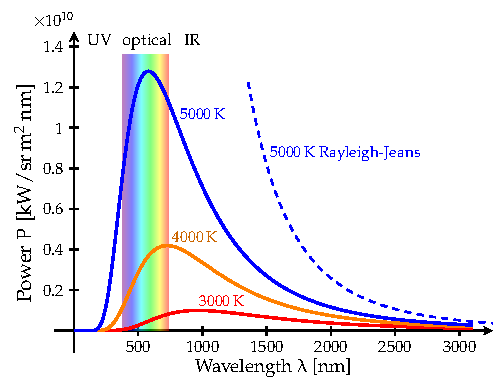
\includegraphics[width=10cm]{images/blackbody.pdf}
  \end{center}
  Anything that has a nonzero absolute temperature radiates some energy. In particular, we want to know how this radiation is distributed among various wavelengths.\newline

  For a box of photons in equilibrium at temperature $T$, the energy per volume per wavelength $\lambda$\footnote{read as (energy per volume) per wavelength} is
  \begin{align*}
    u\left(\lambda\right) &= \frac{8\pi h c}{\lambda^{5}\left(e^{h c/\lambda kT} - 1\right)}.
  \end{align*}
  Here, $h$ denotes Planck's constant, $c$ is the speed of light, and $k$ is Boltzmann's constant.\newline

  In order to find the total energy density, we have to integrate $u(\lambda)$ over all possible values of $\lambda$:
  \begin{align*}
    U &= \int_{0}^{\infty} u\left(\lambda\right)\:d\lambda\\
      &= 8\pi h c\int_{0}^{\infty}\frac{1}{\lambda^{5}\left(e^{hc/\lambda k T} - 1\right)} \:d\lambda
  \end{align*}
  This integral is, for lack of a better word, hard. However, if we remove the dimensions of $\lambda$ by substituting $x = \frac{hc}{\lambda k t}$, we can verify that the value of $U$ now becomes
  \begin{align*}
    U &= 8\pi h c \left(\frac{kT}{hc}\right)^{4}\underbrace{\int_{0}^{\infty} \frac{x^3}{e^x-1}\:dx}_{\text{scalar}}.
  \end{align*}
  Thus, all the physics\footnote{Who cares about that stuff?} is captured as a coefficient on the integral; namely, this integral captures the Stefan--Boltzmann law, which has that energy density scales by $T^{4}$.\newline

  Using some fancy techniques we will learn later, we can evaluate
  \begin{align*}
    \int_{0}^{\infty} \frac{x^3}{e^x-1}\:dx &= \frac{\pi^4}{15}.
  \end{align*}
\end{example}
\subsubsection{Even/Odd}%
\begin{definition}[Even and Odd Functions]
A function $f(x)$ is
\begin{itemize}
  \item even if $f(-x) = f(x)$;
  \item odd if $f(-x) = -f(x)$.
\end{itemize}
\end{definition}
Just as a matrix can be decomposed into a sum of a symmetric and antisymmetric matrix, we can decompose a function into a sum of an even function and an odd function.\newline

Integrals over symmetric intervals on functions with definite parity are very simple:
\begin{align*}
  \int_{-a}^{a} f(x)\:dx &= \begin{cases}
    2\int_{0}^{a} f(x)\:dx & f\text{ odd}\\
    0 & f\text{ even}
  \end{cases}.
\end{align*}
For the case of a function $g\left(x\right) = g\left(|x|\right)$, we have
\begin{align*}
  \int_{-a}^{b} g\left(|x|\right)\:dx &= \int_{-a}^{0} g(-x)\:dx + \int_{0}^{b} g(x)\:dx.
\end{align*}
\subsubsection{Products and Powers of Sines and Cosines}%
\begin{table}
  \centering
  \renewcommand{\arraystretch}{1.5}
  \begin{tabular}{c|c}
    Value & Expression\\
    \hline\hline
    $\sin\left(\alpha \pm \beta\right)$ & $\sin\alpha\cos\beta \pm \sin\beta\cos\alpha$\\
    $\cos\left(\alpha \pm \beta\right)$ & $\cos\alpha\cos\beta \mp \sin\alpha\sin\beta$\\
    \hline
    $\sin\alpha\cos\beta$ & $\frac{1}{2}\left(\sin(\alpha + \beta) + \sin\left(\alpha - \beta\right)\right)$\\
    $\cos\alpha\cos\beta$ & $\frac{1}{2}\left(\cos(\alpha - \beta) + \cos(\alpha + \beta)\right)$\\
    $\sin\alpha\sin\beta$ & $\frac{1}{2}\left(\cos(\alpha - \beta) - \cos(\alpha + \beta)\right)$
  \end{tabular}
  \caption{Useful Trig Identities}
\end{table}
\begin{example}
  If we have an integral
  \begin{align*}
    \int_{}^{} \sin(3x)\cos(2x)\:dx &= \frac{1}{2}\int_{}^{} \sin(5x) + \sin(x)\:dx\\
                                    &= \frac{1}{2}\left(-\frac{1}{5}\cos (5x) - \cos(x) \right).
  \end{align*}
\end{example}
\begin{table}
  \centering
  \renewcommand{\arraystretch}{1.5}
  \begin{tabular}{c|c}
    Integral & Shortcut\\
    \hline\hline
    $\int \sin^{m}(x)\cos^{2k+1}(x)\:dx$ & $\int_{}^{} u^{m}\left(1-u^2\right)^{k}\:du$\\
    $\int_{}^{} \sin^{2k+1}(x)\cos^{n}(x)\:dx$ & $-\int_{}^{} \left(1-u^2\right)^ku^{n}\:du$\\
    $\int_{}^{} \sin^{2}(x)\:dx$ & $\frac{x}{2} - \frac{1}{4}\sin(2x)$\\
    $\int_{}^{} \cos^{2}\left(x\right)\:dx$ & $\frac{x}{2} + \frac{1}{4}\sin(2x)$
  \end{tabular}
  \caption{Integrals of Powers and Products of Sine and Cosine}
\end{table}
\begin{example}
  To evaluate
  \begin{align*}
    \int_{}^{} \sin^{2}(x)\:dx,\\
    \int_{}^{} \cos^2(x)\:dx
  \end{align*}
  we use the identity
  \begin{align*}
    \sin^2(x) &= \frac{1}{2}\left(1-\cos(2x)\right)\\
    \cos^{2}(x) &= \frac{1}{2}\left(1 + \cos(2x)\right),
  \end{align*}
  and take
  \begin{align*}
    \int_{}^{} \sin^2(x)\:dx &= \frac{1}{2}\int_{}^{} \left(1-\cos(2x)\right)\:dx\\
                             &= \frac{x}{2} - \frac{1}{4}\sin(2x)\\
    \int_{}^{} \cos^2(x)\:dx &= \frac{1}{2}\int_{}^{} \left(1+\cos(2x)\right)\:dx\\
                             &= \frac{x}{2} + \frac{1}{4}\sin(2x).
  \end{align*}
  Thus, we can see that
  \begin{align*}
    \int_{0}^{\pi} \sin^2(x)\:dx&= \frac{\pi}{2}\\
    \int_{0}^{\pi} \cos^2(x)\:dx&= \frac{\pi}{2}
  \end{align*}
\end{example}
\subsubsection{Axial and Spherical Symmetry}%
Consider a function of the form $f(x,y) = x^2 + y^2$. If we were to integrate with respect to $dx dy$, we would need a two dimensional integral. With polar coordinates, though, we would have $dx dy = rdrd\phi$. Since $f$ is axially symmetric, we would have our $dx dy = 2\pi r dr$, which is a one-dimensional integral.\newline

If we have something with spherical symmetry, then there is no dependence on either $\theta$ or $\phi$, yielding a function $f\left(\mathbf{r}\right) = f(r)$, meaning
\begin{align*}
  \int_{}^{} f\left(\mathbf{r}\right)\:d\tau &= \int_{}^{} f(r)r^2\sin\theta\:drd\theta d\phi\\
                                             &= 4\pi \int_{}^{} f(r)r^2\:dr.
\end{align*}
Note that $\int_{}^{} \sin\theta \:d\theta d\phi$ over the sphere is $4\pi$.
\begin{example}
  Consider a surface $S$ with charge density $\sigma\left(\mathbf{r}\right)$. Finding the total charge requires evaluating
  \begin{align*}
    Q &= \int_{S}^{} \sigma\left(\mathbf{r}\right)\:dA.
  \end{align*}
  If $S$ is hemispherical with $z > 0$ with radius $R$, and $\sigma = k\frac{x^2 + y^2}{R^2}$, the integrand is axially symmetric.\newline

  Using spherical coordinates, we evaluate
  \begin{align*}
    Q &= \int_{S}^{} \sigma\left(\mathbf{r}\right)\:dA\\
      &= \frac{k}{R^2}\int_{}^{} x^2 + y^2\:dA\\
      &= \frac{k}{R^2}\int_{}^{} \left(R^2\sin^2\theta\cos^2\phi + R^2\sin^2\theta\sin^2\phi\right)R^2\sin\theta\:d\theta d\phi\\
      &= kR^2\int_{S}^{} \sin^{3}\theta\:d\theta d\phi\\
      &= 2\pi kR^2 \int_{0}^{\pi/2} \sin^{3}\theta\:d\theta\\
      &= \frac{4\pi kR^2}{3}.
  \end{align*}
\end{example}
\begin{example}
  Let
  \begin{align*}
    \Phi\left(\mathbf{r}\right) &= \int_{}^{} \frac{e^{-i\mathbf{k}\cdot\mathbf{r}}}{\left(2\pi\right)^3\norm{\mathbf{k}}^2}\:d^{3}k
  \end{align*}
  where $k$-space is an abstract $3$-dimensional Euclidean space. In Cartesian coordinates, $d^3k = dk_x dk_y dk_z$, which yields the integral
  \begin{align*}
    \Phi\left(\mathbf{r}\right) &= \int_{}^{} \frac{e^{-ik_x x}e^{-ik_y y}e^{-ik_z z}}{\left(2\pi\right)^3 \left(k_x^2 + k_y^2 + k_z^2\right)}\:dk_x dk_y dk_z.
  \end{align*}
  This integral is very hard to evaluate (over Cartesian coordinates, anyway),\footnote{Citation needed.} so we need to use some other methods.\newline

  In spherical coordinates, we have $d^3 k = k^2 dk d\Omega$, yielding
  \begin{align*}
    \Phi\left(\mathbf{r}\right) &= \frac{1}{\left(2\pi\right)^3}\int_{}^{} k^2\frac{e^{-ikr\cos\theta}}{k^2}\:dkd\left(\cos \theta\right)d\phi.
  \end{align*}
  Since we are summing away all our $k$-dependence, we can orient $r$ along the $k_z$ axis. Thus, we can evaluate the integral as
  \begin{align*}
    \Phi\left(\mathbf{r}\right) &= \frac{1}{\left(2\pi\right)^3}\int_{}^{} k^2\frac{e^{-ikr\cos\theta}}{k^2}\:dkd\left(\cos \theta\right)d\phi\\
                                &= \frac{1}{\left(2\pi\right)^{2}}\int_{-1}^{1}\int_{0}^{\infty} e^{-ikr\cos\theta} \:dk d(\cos\theta)\\
                                &= \frac{1}{\left(2\pi\right)^2}\int_{}^{} \frac{1}{\left(-ikr\right)}\left(e^{-ikr} - e^{ikr}\right)\:dk\\
                                &= \frac{1}{\left(2\pi\right)^2}\int_{0}^{\infty}\frac{2\sin(kr)}{kr} \:dk\\
                                &= \frac{1}{2\pi^2}\underbrace{\int_{0}^{\infty} \frac{\sin(kr)}{kr}\:dk}_{\text{sinc integral}}.
  \end{align*}
  In order to evaluate the sinc integral, we have to use some different techniques.
\end{example}
\subsubsection{Differentiation with Respect to a Parameter}%
\begin{example}
  We can evaluate
  \begin{align*}
    \int_{}^{} xe^{ax}\:dx &= \pd{}{a}\left(\int_{}^{} e^{ax}\:dx\right)\\
                           &= \pd{}{a} \left(\frac{1}{a}e^{ax}\right)\\
                           &= -\frac{1}{a^2}e^{ax} + \frac{1}{a}xe^{ax}\\
                           &= \frac{1}{a^2}e^{ax}\left(ax - 1\right)
  \end{align*}
  When differentiating with respect to a parameter, it is important to remember that we are often differentiating \textit{with respect to the parameter}, not with respect to our main variable.
\end{example}
\begin{example}[Introducing a Parameter]
  We wish to solve the sinc integral,
  \begin{align*}
    \int_{0}^{\infty} \frac{\sin x}{x}\:dx.
  \end{align*}
  In order to do this, we will introduce a parameter such that differentiation will cancel out the $x$ in the denominator:
  \begin{align*}
    J\left(\alpha\right) &= \int_{0}^{\infty} e^{-\alpha x}\frac{\sin x}{x}\:dx. \tag*{$\alpha > 0$}
  \end{align*}
  In particular, $\alpha > 0$. We calculate
  \begin{align*}
    \frac{dJ}{d\alpha} &= -\int_{0}^{\infty} e^{-\alpha x}\sin x\:dx\\
                       &= -\frac{1}{1 + \alpha^2}.
  \end{align*}
  Therefore,
  \begin{align*}
    J\left(\alpha\right) &= -\int_{}^{} \frac{1}{\alpha^2}\:d\alpha\\
                         &= -\arctan\left(\alpha\right) + C.
  \end{align*}
  In order to determine the value of $C$, we need to make sure $J(\infty) = 0$. Therefore, $C = \frac{\pi}{2}$. Therefore, we have
  \begin{align*}
    J(0) &= \frac{\pi}{2}.
  \end{align*}
\end{example}
\subsubsection{Gaussian Integral}%
We cannot evaluate $I_0 = \int_{0}^{\infty} e^{-ax^2}\:dx$ using elementary methods, because $e^{-ax^2}$ is not an elementary function. The reason we care a lot about $e^{-ax^2}$ is because it is very important in quantum mechanics and statistics.\footnote{Who cares about that?}\newline

It is clear that $I_0$ converges. We can see that the dimension of $a$ is $x^{-2}$, and since we are integrating with respect to $dx$, we can see that our integral is related to $\frac{1}{\sqrt{a}}$.
\begin{example}
  We will not solve for $I_0$, but for $I_0^2$. Thus, we have
  \begin{align*}
    I_0^2 &= \left(\frac{1}{2}\int_{-\infty}^{\infty} e^{-ax^2}\:dx\right)\left(\frac{1}{2}\int_{-\infty}^{\infty} e^{-ay^2}\:dy\right)\\
          &= \frac{1}{4}\int_{-\infty}^{\infty}\int_{-\infty}^{\infty} e^{-a\left(x^2 + y^2\right)}\:dxdy\\
          &= \frac{1}{4}\int_{0}^{2\pi}\int_{0}^{\infty} re^{-ar^2}\:drd\phi\\
          &= \frac{\pi}{2}\int_{0}^{\infty} re^{-ar^2}\:dr\\
          &= \frac{\pi}{2}\left(\frac{1}{2}\int_{0}^{\infty} e^{-au}\:du\right)\\
          &= \frac{\pi}{4a}.
  \end{align*}
  Therefore, $I_0 = \frac{1}{2}\sqrt{\frac{\pi}{a}}$.
\end{example}
\begin{definition}[Family of Gaussian Integrals]
\begin{align*}
  I_n &= \int_{0}^{\infty} x^ne^{-ax^2}\:dx.
\end{align*}
\end{definition}
\begin{table}
  \centering
  \renewcommand{\arraystretch}{1.5}
  \begin{tabular}{c|c}
    Expression & Value\\
    \hline\hline
    $I_0$ & $\frac{1}{2}\sqrt{\frac{\pi}{a}}$\\
    $I_1$ & $\frac{1}{2a}$\\
    $I_{2n}$ & $(-1)^{n}\frac{d^{n}}{da^{n}}I_0$\\
    $I_{2n+1}$ & $\left(-1\right)^{n}\frac{d^{n}}{da^{n}}I_1$
  \end{tabular}
  \caption{Gaussian Integrals}
\end{table}
It is important to note that there are different expressions for the Gaussian integral:
\begin{align*}
  \int_{}^{} e^{-ax^2}\:dx\\
  \int_{}^{} e^{-a^2x^2}\:dx\\
  \int_{}^{} e^{-a^2x^2/2}\:dx\\
  \int_{}^{} e^{-x^2/a}\:dx\\
  \int_{}^{} e^{-x^2/a^2}\:dx,
\end{align*}
meaning we have to be careful when evaluating these integrals.
\begin{example}[Error Function]
Consider the integral
\begin{align*}
  \int_{0}^{53} e^{-ax^2}\:dx.
\end{align*}
Unfortunately, there is no way to do this integral analytically. It is only able to be calculated numerically.\newline

We define
\begin{align*}
  \text{erf}\left(u\right) &= \int_{0}^{u} e^{-ax^2}\:dx
\end{align*}
\end{example}
\subsubsection{Completing the Square}%
\begin{example}
  Consider the integral
  \begin{align*}
    \int_{-\infty}^{\infty} e^{-ax^2-bx}\:dx.
  \end{align*}
  This integral is Gaussian-esque, but it isn't fully Gaussian, yet.\newline

  To do this, we will complete the square:
  \begin{align*}
    ax^2 + bx &= a\left(x^2 + \frac{b}{a}x\right)\\
              &= a\left(x^2 + \frac{b}{a}x + \frac{b^2}{4a^2} - \frac{b^2}{4a^2}\right)\\
              &= a\left(x + \frac{b}{2a}\right)^2 - \frac{b^2}{4a}.
  \end{align*}
  In particular, this turns the integral into
  \begin{align*}
    \int_{-\infty}^{\infty} e^{-ax^2 - bx}\:dx &= \int_{-\infty}^{\infty} e^{-a\left(x + b/2a\right)^2 + b^2/4a}\:dx\\
                                               &= e^{b^2/4a}\int_{-\infty}^{\infty} e^{-a\left(x + b/2a\right)}\:dx\\
                                               &= e^{b^2/4a}\left(\sqrt{\frac{\pi}{a}}\right)\\
                                               &= e^{b^2/4a}\sqrt{\frac{\pi}{a}}.
  \end{align*}
\end{example}
\subsubsection{Series Expansion}%
\begin{table}
  \centering
  \renewcommand{\arraystretch}{1.75}
  \begin{tabular}{c|c}
    Function & Expression\\
    \hline\hline
    $\Gamma(s)$ & $\displaystyle \int_{0}^{\infty} x^{s-1}e^{-x}\:dx$\\
    $\zeta(s)$ & $\displaystyle \sum_{k=1}^{\infty}\frac{1}{k^s}$\\
    $\Gamma\left(s+1\right)$ & $s\Gamma(s)$
  \end{tabular}
  \caption{Gamma and Zeta Functions}
\end{table}
Consider the integral
\begin{align*}
  \int_{0}^{\infty} \frac{x^{s-1}}{e^{x}-1}\:dx.
\end{align*}
This is a very nasty integral,\footnote{Citation needed.} but we will need to know this value because it is useful in statistical mechanics.\footnote{Okay actually I do kinda care about this.} We want to ensure this converges.\newline

Notice that for large $x$, the integrand looks like $e^{-x}x^{s-1}$.
\begin{example}
  To resolve the integral we take
  \begin{align*}
    \int_{0}^{\infty} \frac{x^{s-1}}{e^{x}-1}\:dx &= \int_{0}^{\infty} \frac{e^{-x}x^{s-1}}{1-e^{-x}}\:dx
    \intertext{We will use the geometric series expansion for the denominator:}
                                                  &= \int_{0}^{\infty} e^{-x}x^{s-1}\sum_{k=0}^{\infty}e^{-kx}\:dx\\
                                                  &= \sum_{k=0}^{\infty}\int_{0}^{\infty} x^{s-1}e^{-\left(k+1\right)x}\:dx.
                                                  \intertext{We make the change of variables $u = (n+1)x$.}
                                                  &= \sum_{n=0}^{\infty}\frac{1}{\left(n+1\right)^{s}}\int_{0}^{\infty} u^{s-1}e^{-u}\:du\\
                                                  &= \underbrace{\sum_{n=1}^{\infty}\frac{1}{n^s}}_{\zeta(s)}\underbrace{\int_{0}^{\infty} u^{s-1}e^{-u}\:du}_{\Gamma(s)}.
  \end{align*}
  Thus, our integral resolves to
  \begin{align*}
    \int_{0}^{\infty} \frac{x^{s-1}}{e^{x}-1}\:dx &= \Gamma(s)\zeta(s).
  \end{align*}
\end{example}
\subsubsection{Partial Fractions}%
\begin{example}[A Partial Fraction Decomposition]
  \begin{align*}
    \frac{1}{1-x^2} &= \frac{\alpha}{1-x} + \frac{\beta}{1+x}\\
                    &= \frac{1/2}{1-x} + \frac{1/2}{1+x}.
  \end{align*}
\end{example}
\begin{example}[Integrating using Partial Fractions]
  To evaluate
  \begin{align*}
    \int_{}^{} \frac{4-2x}{\left(x^2 + 1\right) \left( x-1\right)^2}\:dx,
  \end{align*}
  we do the partial fraction decomposition to find
  \begin{align*}
    \int_{}^{} \frac{4-2x}{\left(x^2 + 1\right) \left( x-1\right)^2}\:dx &= \int_{}^{} \frac{2x+1}{x^2 + 1} + \frac{-2}{x-1} + \frac{1}{\left(x-1\right)^2}\:dx.
  \end{align*}
\end{example}
\begin{example}[Mean Value Theorem]
  If we have a function $f$ defined on $[a,b]$, then there is a point $c\in \left(a,b\right)$ such that
  \begin{align*}
    f(c)\left(b-a\right) &= \int_{a}^{b} f(x)\:dx.
  \end{align*}
  More generally, the mean value theorem says there exists $c\in \left(a,b\right)$ such that
  \begin{align*}
    \int_{a}^{b} f(x)g(x)\:dx &= f(c)\int_{a}^{b} g(x)\:dx
  \end{align*}
\end{example}
\subsection{Delta Distribution}%
Consider a ``function'' $\delta(x)$ such that
\begin{align*}
  \int_{-\infty}^{\infty} f(x)\delta(x-a)\:dx &= f(a).
\end{align*}
This idea seems absurd on its face --- after all, singletons have measure zero, so the idea of an integral collapsing into a single point doesn't sound normal.\newline

The structure of the delta distribution is
\begin{align*}
  \delta\!\left(x-a\right) &= \begin{cases}
    +\infty & x=a\\
    0 & \text{else}
  \end{cases}.
\end{align*}
In particular, we also have to define
\begin{align*}
  \int_{-\infty}^{\infty} \delta\!\left(x-a\right)\:dx &= 1.
\end{align*}
This is known as the Dirac delta function (or rather, distribution). The delta distribution ``weights'' $f$ to infinity at $x=a$ and zero everywhere else.
\begin{example}[Delta Distribution as a Limit]
  Imagine a Gaussian function with area under the curve $1$. In particular,
  \begin{align*}
    f_n(x) &= \frac{1}{\sqrt{\pi}}ne^{-n^2x^2}.
  \end{align*}
  In particular, we have
  \begin{align*}
    \delta(x) &= \lim_{n\rightarrow\infty}\frac{1}{\sqrt{\pi}}ne^{-n^2x^2}
  \end{align*}
\end{example}
\begin{example}[A Physical Example]
  Imagine a ball is kicked. The force is dependent on time, $F(t)$.\newline

  There isn't an easy to find the force, but by Newton's second law, we have
  \begin{align*}
    \delta p &= \int_{}^{} F(t)\:dt,
  \end{align*}
  where
  \begin{align*}
    I \equiv \int_{}^{} F(t)\:dt
  \end{align*}
  is the impulse.\newline

  If we want to model $F(t)$, where we don't care about a nonzero time over which the force is occurring, we can simply state $F(t)$ as
  \begin{align*}
    F(t) &= \Delta p \delta\!\left(t-t_0\right).
  \end{align*}
  Taking this integral yields $I$.
\end{example}
\begin{example}[Fourier Integral Representation of Delta Distribution]
A different representation of $\delta(x)$ is
\begin{align*}
  \delta(x) &= \frac{1}{2\pi}\int_{-\infty}^{\infty} e^{ikx}\:dk.
\end{align*}
We are superimposing all the waves $e^{ikx}$ --- in particular, for all values of $k\neq 0$, both $e^{ikx}$ and $e^{-ikx}$ are ``added'' together, yielding absolute destructive interference.\newline

The factor of $\frac{1}{2\pi}$ is necessary to normalize the integral.
\end{example}
\subsubsection{Properties of the Delta Distribution}%
\begin{description}[leftmargin=0pt]
  \item[Normalization:]
    \begin{align*}
      \int_{-\infty}^{\infty} \delta(x)\:dx &= 1\\
      \int_{x_1}^{x_2} \delta(x-a)\:dx &= \begin{cases}
        1 & x_1 < a < x_2\\
        0 & \text{else}
      \end{cases}.
    \end{align*}
  \item[Sieve:]
    \begin{align*}
      \int_{x_1}^{x_2} f(x)\delta(x-a)\:dx &= \begin{cases}
        f(a) & x_1 < a < x_2\\
        0 & \text{else}
      \end{cases}.
    \end{align*}
\end{description}
\begin{example}[Delta Distribution as a Limit of Rectangles]
  We define the family of functions
  \begin{align*}
    \phi_k(x) &= \begin{cases}
      k/2 & |x| < 1/k\\
      0 & |x| > 1/k
    \end{cases}.
  \end{align*}
  We can see that integrating $\phi_k$ over $\R$ yields $1$ for each $k$.\newline

  We now need to evaluate if $\lim_{k\rightarrow\infty}\phi_k(x) = \delta(x)$. In order to see this, we take
  \begin{align*}
    \lim_{k\rightarrow\infty}\int_{-\infty}^{\infty} f(x)\phi_k(x)\:dx &= \lim_{k\rightarrow\infty}\frac{k}{2}\int_{-1/k}^{1/k} f(x)\:dx\\
                                                                       &= \lim_{k\rightarrow\infty}f\left(c_k\right)\left(\frac{k}{2}\int_{-1/k}^{1/k} \:dx\right)\\
                                                                       &= \lim_{k\rightarrow\infty}f\left(c_k\right),
  \end{align*}
  where we define $c_k$ from the mean value theorem. In particular, since $c_k \in \left(-1/k,1/k\right)$, it is the case that $c_k\rightarrow 0$ as $k\rightarrow\infty$, so
  \begin{align*}
    \lim_{k\rightarrow\infty}\int_{-\infty}^{\infty} f(k)\phi_k(x)\:dx &= \lim_{k\rightarrow\infty}f\left(c_k\right)\\
                                                                       &= f(0).
  \end{align*}
  Thus, $\lim_{k\rightarrow\infty}\phi_k(x) = \delta(x)$.
\end{example}
We can imagine the delta distribution to be the density distribution of a single point.\newline

The units of $\delta(x)$ are
\begin{align*}
  \left[\delta(x)\right] &= x^{-1}.
\end{align*}
\begin{example}[Linear Argument for $\delta$]
Consider $\delta\!\left(ax\right)$. For instance, we want to evaluate
    \begin{align*}
      \int_{-\infty}^{\infty} f(x)\delta(ax)\:dx.
    \end{align*}
    To do so, we use $u$ substitution with $u = ax$:
    \begin{align*}
      \int_{-\infty}^{\infty} f(x)\delta\!\left(ax\right)\:dx &= \frac{1}{a}\int_{-\infty}^{\infty} f\left(u/a\right)\delta(u)\:du\\
                                                            &= \frac{1}{a}f(0).
    \end{align*}
    It is important to note that the integration variable $dx$ and the argument of $\delta(x)$ must be equal.\newline

    In general, we have
    \begin{align*}
      \delta(ax) &= \frac{1}{|a|}\delta(x).
    \end{align*}

\end{example}
\begin{example}[Function Argument for $\delta$]
  We now want to evaluate
  \begin{align*}
    \int_{-\infty}^{\infty} f() \delta(g(x))\:dx.
  \end{align*}
  When we take the change of variables, we have
  \begin{align*}
    \int_{y_1}^{y_2} f(y)\delta(y)\:dy &= \int_{x_1}^{x_2} f(g(x))\delta(g(x)) \left\vert \frac{dg}{dx} \right\vert\:dx.
  \end{align*}
  Therefore, we must have $\delta(g(x)) = \frac{1}{\left\vert dg/dx \right\vert_{g(x)=0}}\delta(x)$.\newline

  In the general case, we have
  \begin{align*}
    \delta\!\left(g(x)\right) &= \frac{1}{\left\vert dg/dx \right\vert_{x_0}}\delta\!\left(x-x_0\right)
  \end{align*}
  where $g\left(x_0\right) = 0$.\newline

  If, in the region of integration, $g$ takes multiple zeros, we must take a sum:
  \begin{align*}
    \delta\!\left(g(x)\right) &= \sum_{i}\frac{1}{\left\vert dg/dx \right\vert_{x_i}}\delta\!\left(x_i\right);
  \end{align*}
  where we assume $\left\vert \frac{dg}{dx} \right\vert_{x_i} \neq 0$.
\end{example}
\begin{example}[$x^2 - a^2$ Argument for $\delta$]
  Consider the distribution
  \begin{align*}
    \delta\!\left(x^2 - a^2\right).
  \end{align*}
  The derivative of $g(x)$ is $2x$; the two zeros of $g$ are at $x = \pm a$. Therefore,
  \begin{align*}
    \delta\!\left(x^2 - a^2\right) &= \frac{1}{\left\vert 2x \right\vert_{a}}\delta\!\left(x-a\right) + \frac{1}{\left\vert 2x \right\vert_{-a}}\delta\!\left(x+a\right)\\
                                 &= \frac{1}{2a}\left(\delta\!\left(x-a\right) + \delta\!\left(x+a\right)\right).
  \end{align*}
  For example, if we took
  \begin{align*}
    \int_{-\infty}^{\infty} x^3\delta\!\left(x^2 - a^2\right)\:dx &= \frac{1}{2a}\int_{-\infty}^{\infty} x^3\left(\delta\!\left(x-a\right) + \delta\!\left(x+a\right)\right)\:dx\\
                                                                &= \frac{1}{2a}\left(a^3 + \left(-a\right)^3\right)\\
                                                                &= 0.
  \end{align*}
  Now, evaluating
  \begin{align*}
    \int_{0}^{\infty} x^3\left(\delta\!\left(x^2 - a^2\right)\right)\:dx &= \frac{1}{2a}\int_{0}^{\infty} x^3\left(\delta\!\left(x-a\right) + \delta\!\left(x+a\right)\right)\:dx\\
                                                                       &= \frac{1}{2a}\left(a^3\right)\\
                                                                       &= \frac{1}{2}a^2.
  \end{align*}
\end{example}
\begin{example}[(Weak) Derivative of $\delta$]
  Obviously we cannot formally take $\delta'(x)$, but we can always place $\delta(x)$ under the integral sign and treat $\delta'(x)$ as the ``derivative'' via integration by parts:
  \begin{align*}
    \int_{-\infty}^{\infty} f(x)\delta'(x)\:dx &= f(x)\delta(x)\bigr\vert_{-\infty}^{\infty} - \int_{-\infty}^{\infty} \frac{df}{dx}\delta(x)\:dx\\
                                               &= -\frac{df}{dx}\bigr\vert_{0}\\
                                               &= -f'(0).
  \end{align*}
  The ``identity'' for the delta function's derivatives is
  \begin{align*}
    f(x) \delta'(x) &= -f'(x)\delta(x).
  \end{align*}
\end{example}
\begin{example}[Heaviside Step Function]
The Heaviside step function, $\Theta(x)$, is
\begin{align*}
  \Theta(x) &= \begin{cases}
    0 & x < 0\\
    1 & x > 0.
  \end{cases}
\end{align*}
\begin{center}
  \begin{tikzpicture}
    \draw[thick] (-3,0) -- (0,0);
    \draw[thick] (0,1) -- (3,1);
    \draw (0,3) -- (0,-1);
    \draw (-3,0) -- (3,0);
  \end{tikzpicture}
\end{center}
\end{example}
\begin{example}[Higher Dimension Delta Distributions]
  In higher dimensions,
  \begin{align*}
    \int_{\text{all space}}^{} \delta\!\left(\mathbf{r}\right)\:d\tau &= 1,
  \end{align*}
  and
  \begin{align*}
    \int_{V}^{} f\left(\mathbf{r}\right)\delta\!\left(\mathbf{r}-\mathbf{a}\right)\:d\tau &= \begin{cases}
      f\left(\mathbf{a}\right) & \mathbf{a}\in V\\
      0 & \text{otherwise}
    \end{cases}.
  \end{align*}
  One of the common notations for higher dimensional delta functions is $\delta^{(n)}\left(\mathbf{r}\right)$, where $(n)$ denotes the dimension (not to be confused with $n$th derivative).\newline

  Instead, we can use $\delta\!\left(\mathbf{r}\right)$, which lets us know that we are dealing in higher dimensions, and context is evident.
\end{example}
\begin{example}[Voltage under a Point Charge]
  The voltage of a point charge $q$ at a position $\mathbf{a}$ is given by Coulomb's law
  \begin{align*}
    \Phi(\mathbf{r}) &= \frac{q}{4\pi \epsilon_0} \frac{1}{\left\vert \mathbf{r} - \mathbf{a} \right\vert},
  \end{align*}
  with $\Phi = 0$ at $\infty$.\newline

  For a continuous point charge distribution $\rho\left(\mathbf{r}\right)$, we consider each element of the volume $d\tau$ centered at $\mathbf{r}$ with charge $dq = \rho\left(\mathbf{r}\right)d\tau$.
  \begin{align*}
    d\Phi\left(\mathbf{r}\right) &= \frac{dq}{4\pi \epsilon_0}\frac{1}{\left\vert \mathbf{r} - \mathbf{a} \right\vert}\\
                                 &= \frac{1}{4\pi\epsilon_0}\frac{\rho\left(\mathbf{r}\right)d\tau}{\left\vert \mathbf{r} - \mathbf{a} \right\vert}.
  \end{align*}
  In particular, for some $\mathbf{r}$, we need to add up over $\mathbf{a}$, yielding
  \begin{align*}
    \Phi\left(\mathbf{r}\right) &= \frac{1}{4\pi\epsilon_0}\int_{V}^{} \frac{\rho\left(\mathbf{r}'\right)}{\left\vert \mathbf{r} - \mathbf{r}' \right\vert}\:d\tau'
  \end{align*}
  This expression should hold for every physically reasonable volume charge distribution $\rho$, what $\rho\left(\mathbf{r}\right)$ denotes a point charge?\newline

  In particular, if $\rho\left(\mathbf{r}\right)$ is a point charge, then $\rho = q\delta\!\left(\mathbf{r} - \mathbf{a}\right)$.
\end{example}
\begin{example}[Using the Multi-Dimensional Delta Distribution]
  In Cartesian coordinates, we have
  \begin{align*}
    \delta\!\left(\mathbf{r} - \mathbf{r}_0\right) &= \delta\!\left(x-x_0\right)\delta\!\left(y-y_0\right)\delta\!\left(z-z_0\right).
  \end{align*}
  If we want to transform $\delta\!\left(\mathbf{r} - \mathbf{r}_0\right)$ into a different coordinate system such as $d\tau = du\:dv\:dw$, we need the Jacobian. Thus,
  \begin{align*}
    \delta\!\left(\mathbf{r} - \mathbf{r}_0\right) &= \frac{1}{|J|}\delta\!\left(u-u_0\right)\delta\!\left(v-v_0\right)\delta\!\left(w-w_0\right).
  \end{align*}
  For instance, in spherical coordinates, we have
  \begin{align*}
    \delta\!\left(\mathbf{r} - \mathbf{r}_0\right) &= \frac{1}{r^2\sin\theta}\delta\!\left(r-r_0\right)\delta\!\left(\theta - \theta_0\right)\delta\!\left(\phi-\phi_0\right)\\
                                                 &= \frac{1}{r^2}\delta\!\left(r-r_0\right)\delta\!\left(\cos\theta - \cos\theta_0\right)\delta\!\left(\phi-\phi_0\right).
  \end{align*}
\end{example}
\section{Vector Calculus}%
\begin{question}
  What is a vector?
\end{question}
\begin{answer}
  A vector is an element of a vector space.
\end{answer}
\begin{remark}
  Yes, vectors as defined by ``magnitude and direction'' also are elements of vector spaces.
\end{remark}
For the purposes of this unit, we will focus on vectors in the vector space $\R^n$ over $\R$.
\begin{notation}
  Vector-valued functions with vector-valued outputs will be denoted
  \begin{align*}
    \mathbf{F}\left(\mathbf{r}\right).
  \end{align*}
\end{notation}
\subsection{Vector Fields}%
\begin{definition}[Vector Field]
  A vector-valued function $\mathbf{F}\left(\mathbf{r}\right)$ with vector-valued outputs is known as a vector field.
\end{definition}
\begin{example}
  The field
  \begin{align*}
  \mathbf{F}\left(x,y,z\right) &= x\hat{i} + y\hat{j} + z\hat{k}
  \end{align*}
  can be seen below.
  \begin{center}
    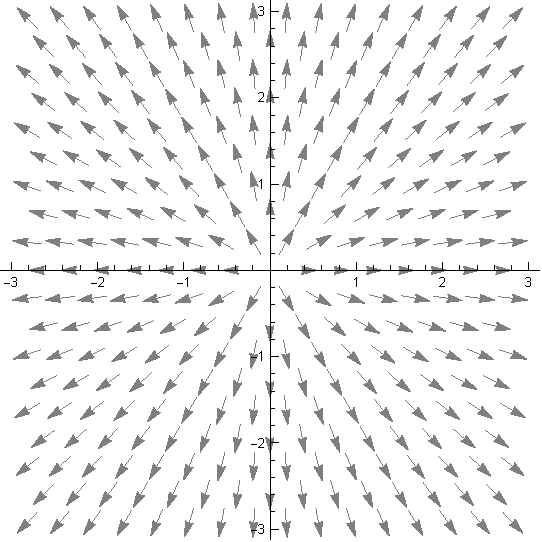
\includegraphics[width=10cm]{images/xyz_vector_field.pdf}
  \end{center}
  Notice that, in terms of spherical coordinates, $\mathbf{F}\left(x,y,z\right) = r\hat{r} = \mathbf{r}$.
\end{example}
\begin{definition}[Incompressible Fluid]
  A fluid is incompressible if its density is constant.\newline

  In particular, incompressible fluids cannot have either sources or sinks, since sources imply a local reduction in density, while sinks imply a local increase in density.
\end{definition}
\begin{example}
  Consider a sprinkler with $N$ streams. Since water is incompressible, the density of streamlines $\sigma$ and the surface area of the spherical shells, $A$ must be inversely proportional to each other.
  \begin{center}
    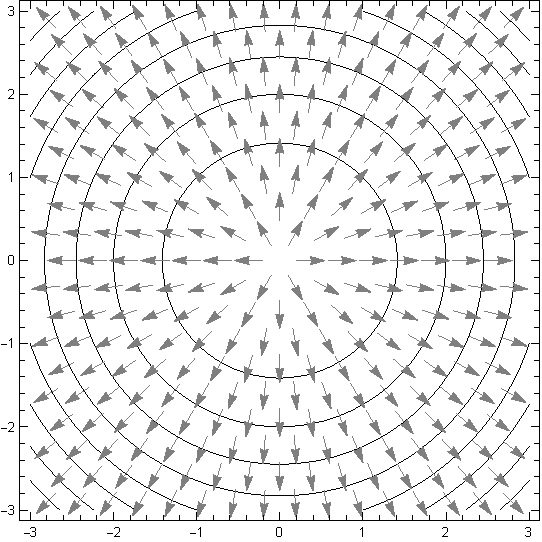
\includegraphics[width=10cm]{images/shells_vector_field.pdf}
  \end{center}
  Thus, we have
  \begin{align*}
    N &=\sigma A,
  \end{align*}
  meaning $\sigma \sim \frac{1}{r^2}$ since $A\sim r^2$.\newline

  In particular, the strength of the vector field must diminish with the square of the distance.
  \begin{center}
    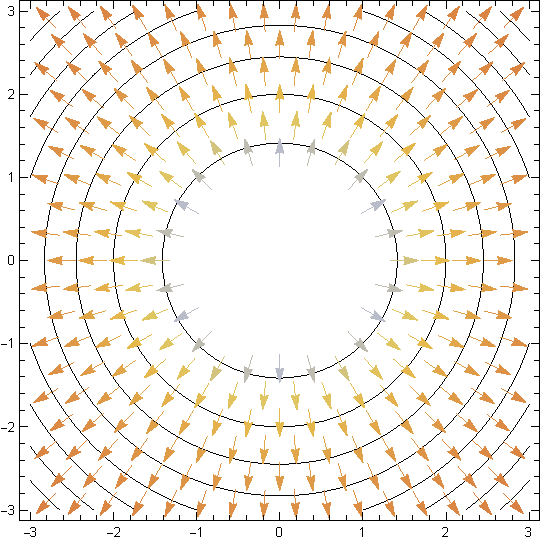
\includegraphics[width=10cm]{images/shells_vector_field_2.pdf}
  \end{center}
\end{example}
\begin{example}
  Vector fields can be added.
  \begin{center}
    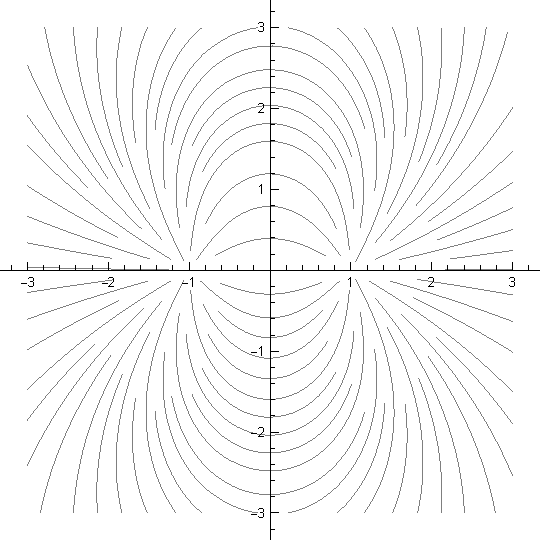
\includegraphics[width=10cm]{images/dipoles.pdf}
  \end{center}
\end{example}
\begin{example}
  Consider the field
  \begin{align*}
    \mathbf{G}\left(x,y\right) &= \frac{1}{\sqrt{x^2 + y^2}}\left(-y\hat{i} + x\hat{j}\right)
  \end{align*}
  As depicted, we can see that the vector field looks as follows.
  \begin{center}
    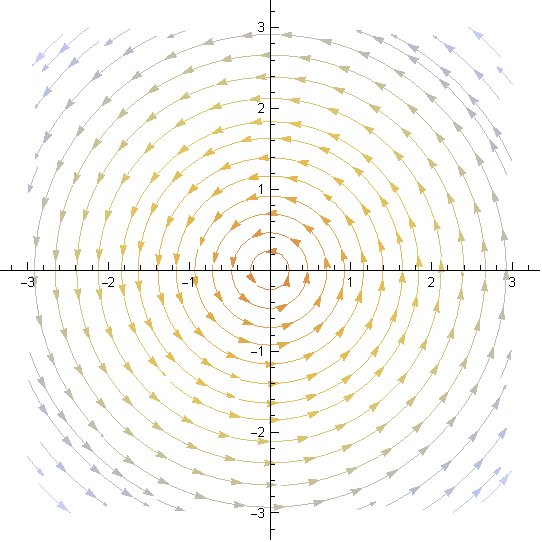
\includegraphics[width=10cm]{images/phihat_field.pdf}
  \end{center}
  In particular, we can see that $\mathbf{G} = \hat{\phi}$.
\end{example}
Notice that our vector fields are dependent on both the basis and the coordinate system.\newline

In particular, we have reason to prefer a Cartesian basis over the polar or spherical basis, since the Cartesian basis is position-independent.
\subsection{Gradient, Divergence, and Curl}%
\begin{table}
  \centering
  \renewcommand{\arraystretch}{1.5}
  \begin{tabular}{c|c|c}
    Value & Expression In Terms of $\nabla$ & Expression In Terms of $\partial$\\
    \hline\hline
    Gradient & $\nabla f$ & $\pd{f}{x} \hat{i} + \pd{f}{y}\hat{j} + \pd{f}{z}\hat{k}$\\
    Divergence & $\nabla \cdot \mathbf{E}$ & $\sum_{i}\partial_i E_i$\\
    Curl & $\nabla \times \mathbf{B}$ & $\sum_{i,j,k}\epsilon_{ijk}\partial_{i}B_j\hat{e}_k$\\
    Laplacian of a scalar field & $\nabla^2 f$ & $\sum_{i}\frac{\partial^2}{\partial i^2}f$\\
    Laplacian of a vector field & $\nabla^2\mathbf{v}$ & $\sum_{i}\pd{^2}{i^2}v_i \hat{e}_i$
  \end{tabular}
  \caption{Gradient, Divergence, and Curl}
\end{table}
\subsubsection{The $\nabla$ Operator}%

Consider a scalar function $f\left(\mathbf{r}\right)$. If we want to imagine how $f$ changes as we move $\mathbf{r}$ to $\mathbf{r} + d\mathbf{r}$, we use the chain rule.
\begin{align*}
  df &= \left(\pd{f}{x}\right)dx + \left(\pd{f}{y}\right)dy + \left(\pd{f}{z}\right)dz\\
     &= \begin{pmatrix}\frac{\partial f}{\partial x}\\\frac{\partial f}{\partial y}\\\frac{\partial f}{\partial z}\end{pmatrix} \begin{pmatrix}dx\\dy\\dz\end{pmatrix}\\
     &= \nabla f \cdot d\mathbf{r}.
\end{align*}
In particular, we define
\begin{align*}
  \nabla f &= \pd{f}{x} \hat{i} + \pd{f}{y}\hat{j} + \pd{f}{z}\hat{k}.
\end{align*}
Notice that, since $dx\hat{i} + dy\hat{j} + dz\hat{k}$ is a vector, and $df$ is a scalar, we know that $\nabla f$ \textit{must} be a vector.
\begin{definition}[Gradient]
  \begin{align*}
    \nabla f &= \pd{f}{x} \hat{i} + \pd{f}{y}\hat{j} + \pd{f}{z}\hat{k}\\
    df &= \left\vert \nabla f \right\vert \left\vert d\mathbf{r} \right\vert \cos\theta.
  \end{align*}
\end{definition}
If $\nabla f$ is in the direction of $d\mathbf{r}$, then $\cos\theta = 1$, meaning $df$ is maximized. In particular, $\nabla f$ points in the direction of maximum change in $f$.\newline

In particular, this means that for every (differentiable) scalar field, there is a natural vector field associated with the direction of largest increase.
\begin{example}
  The electric field
  \begin{align*}
    \mathbf{E} &= -\nabla V.
  \end{align*}
  Similarly, for any given potential $U$, 
  \begin{align*}
    \mathbf{F} &= -\nabla U.
  \end{align*}
\end{example}
\begin{definition}[The $\nabla$ Operator]
  \begin{align*}
    \nabla f &= \begin{pmatrix}\pd{f}{x}\\\pd{f}{y}\\\pd{f}{z}\end{pmatrix}\\
             &= \underbrace{\begin{pmatrix}\pd{}{x}\\\pd{}{y}\\\pd{}{z}\end{pmatrix}}_{\nabla} \left(f\right)
  \end{align*}
  Thus, we get
  \begin{align*}
    \nabla \equiv \pd{}{x}\hat{i} + \pd{}{y}\hat{j} + \pd{}{z}\hat{k}.
  \end{align*}
\end{definition}
\begin{example}\hfill
  \begin{enumerate}[(1)]
    \item For some scalar field $f\left(\mathbf{r}\right)$, we can take
      \begin{align*}
        \nabla\left(f\right) &= \nabla f,
      \end{align*}
      which yields the gradient field.
    \item For some vector field $\mathbf{E}$, we can take
      \begin{align*}
        \nabla \cdot \mathbf{E} = g
      \end{align*}
      which yields a scalar field known as the divergence of $\mathbf{E}$.\newline

      In particular,
      \begin{align*}
        \nabla \cdot \mathbf{E} &= \pd{}{x}\left(\mathbf{E}\cdot \hat{i}\right) + \pd{}{y}\left(\mathbf{E}\cdot \hat{j}\right) + \pd{}{z}\left(\mathbf{E}\cdot \hat{k}\right).
      \end{align*}
    \item For some vector field $\mathbf{B}$, we can take
      \begin{align*}
        \nabla \times \mathbf{B} = \mathbf{A},
      \end{align*}
      which yields a vector field known as the curl of $\mathbf{B}$.
    \item 
      \begin{align*}
        \nabla \cdot \left(\nabla f\right) &= \left(\nabla \cdot \nabla\right) f\\
                                           &= \pd{^2 f}{x^2} + \pd{^2 f}{y^2} + \pd{^2 f}{z^2}\\
                                           &= \nabla^2 f\\
                                          &= \Delta f,
      \end{align*}
      which yields an operator known as the Laplacian.
  \end{enumerate}
\end{example}
\begin{example}
  Let $\mathbf{v}_1 = xy\hat{i} + y^2\hat{j}$. Then,
  \begin{align*}
    \nabla \cdot \mathbf{v}_1 &= \pd{}{x}\left(xy\right) + \pd{}{y}\left(y^2\right)\\
                              &= y + 2y\\
                              &= 3y,
                              \intertext{and}
    \nabla \times \mathbf{v}_1 &= \left(\pd{}{x}\left(y^2\right) - \pd{}{y}\left(xy\right)\right)\hat{k}\\
                               &= -x\hat{k}.
  \end{align*}
\end{example}
\begin{example}
  Let $\mathbf{v}_2 = \frac{1}{x^2 + y^2 + z^2}\left(x\hat{i} + y\hat{j} + z\hat{k}\right)$. Then,
  \begin{align*}
    \nabla \cdot \mathbf{v}_2 &= \pd{}{x}\left(\frac{x}{x^2 + y^2 + z^2}\right) + \pd{}{y}\left(\frac{y}{x^2 + y^2 + z^2}\right) + \pd{}{z}\left(\frac{z}{x^2 + y^2 + z^2}\right)\\
                              &= \frac{1}{x^2 + y^2 + z^2}
    \nabla \times \mathbf{v}_2 &= 0
  \end{align*}
\end{example}
\begin{example}
  Consider
  \begin{align*}
    \mathbf{v} &= x^2 \hat{i} + y^2 \hat{j} + z^2\hat{k}\\
    \mathbf{u} &= yz\hat{i} + zx\hat{j} + xy\hat{k}.
  \end{align*}
  In particular, it is easily verified that $\nabla \times \mathbf{v} = 0$ and $\nabla \cdot \mathbf{u} = 0$.
\end{example}
\subsubsection{Applying Vector Identities to the $\nabla$ Operator}%
We are aware that
\begin{align*}
  a\mathbf{V} &= \mathbf{V}a\\
  \mathbf{A}\cdot \mathbf{B} &= \mathbf{B}\cdot \mathbf{A}.
\end{align*}
However, when we deal with $\nabla$, we have to respect both the properties of the vectors \textit{and} the properties of the operator. In particular,
\begin{align*}
  f\nabla \neq \nabla f.
\end{align*}
This is because $f\nabla$ is a vector operator, while $\nabla f$ is a vector field. Similarly,
\begin{align*}
  \nabla \cdot \mathbf{E} \neq \mathbf{E}\cdot \nabla,
\end{align*}
since $\nabla \cdot \mathbf{E}$ is a scalar field, while $\mathbf{E}\cdot \nabla$ is a scalar operator.
\begin{example}[Curl of Curl]
  Consider
  \begin{align*}
    \nabla \times \left(\nabla \times \mathbf{v}\right).
  \end{align*}
  On first glance, we want to use the identity $\mathbf{A}\times \left(\mathbf{B}\times \mathbf{C}\right) = \mathbf{B}\left(\mathbf{A}\cdot \mathbf{C}\right) - \mathbf{C}\left(\mathbf{A}\times \mathbf{B}\right)$, yielding
  \begin{align*}
    \nabla \times \left(\nabla \times \mathbf{v}\right) &= \nabla\left(\nabla \cdot \mathbf{v}\right) - \mathbf{v}\left(\nabla \cdot \nabla\right).
  \end{align*}
  However, notice that $\mathbf{v}\left(\nabla \cdot \nabla\right)$ is a scalar operator, while $\nabla \times \left(\nabla \times \mathbf{v}\right)$ is a vector field. Thus, we have to modify the double cross product to $\mathbf{A}\times \left(\mathbf{B}\times \mathbf{C}\right) = \mathbf{B}\left(\mathbf{A}\cdot \mathbf{C}\right) - \left(\mathbf{A}\times \mathbf{B}\right)\mathbf{C}$
  \begin{align*}
    \nabla \times \left(\nabla \times \mathbf{v}\right) &= \nabla\left(\nabla \times \mathbf{v}\right) - \nabla^2 \mathbf{v}.
  \end{align*}
\end{example}
\begin{example}[Curl of Gradient and Divergence of Curl]
  Consider
  \begin{align*}
    \nabla \times \left(\nabla f\right).
  \end{align*}
  In particular, we are tempted to take
  \begin{align*}
    \nabla \times \left(\nabla f\right) &= \left(\nabla \times \nabla\right)f\\
                                        &= 0.
  \end{align*}
  This is allowed, since we do not affect the property of the operation.\newline

  The following identity is also true,
  \begin{align*}
    \nabla \cdot \left(\nabla \times \mathbf{v}\right) &= 0,
  \end{align*}
  but we cannot use a cheesy method to prove this.
\end{example}
\begin{remark}
  Faraday's law is $\nabla \times \mathbf{E} = 0$, and Gauss's law for magnetism is $\nabla \times \mathbf{B} = 0$, where $\mathbf{E}$ denotes the electric field and $\mathbf{B}$ denotes the magnetic field.\newline

  If $\nabla \times \mathbf{E} = 0$ in electrostatics, then $\mathbf{E} = \nabla A$ for some scalar function $A$. In particular, we say $\mathbf{E} = -\nabla V$. We call $V$ the scalar potential.\newline

  Similarly, if $\nabla \cdot \mathbf{B} = 0$, then $\mathbf{B} = \nabla \times \mathbf{A}$ for some vector field $\mathbf{A}$. We call $\mathbf{A}$ the vector potential.
\end{remark}
\begin{example}[Products]
  Consider
  \begin{align*}
    \nabla \left(fg\right).
  \end{align*}
  Using the product rule, we have
  \begin{align*}
    \nabla \left(fg\right) &= \left(\nabla f\right)g + f\left(\nabla g\right).
  \end{align*}
  However, when we look at
  \begin{align*}
    \nabla \cdot \left(f\mathbf{A}\right),
  \end{align*}
  things get a little more complicated. Notice that $\nabla \cdot \left(f\mathbf{A}\right)$ is a scalar, meaning we apply the product rule using dot products to yield such a scalar.
  \begin{align*}
    \nabla \cdot \left(f\mathbf{A}\right) &= \nabla f \cdot \mathbf{A}  + f\nabla\cdot \mathbf{A}.
  \end{align*}
  Similarly,
  \begin{align*}
    \nabla \times \left(\mathbf{A}f\right) &= \left(\nabla \times \mathbf{A}\right)f + \nabla f \times \mathbf{A}\\
                                           &= \left(\nabla \times \mathbf{A}\right)f - \mathbf{A}\times \nabla f.
  \end{align*}
\end{example}
\subsubsection{Changing Coordinates}%
\begin{table}
  \scriptsize
  \centering
  \renewcommand{\arraystretch}{2}
  \begin{tabular}{c|c|c}
    Coordinate System & Value & Expression\\
    \hline\hline
    \multirow[c]{4}{*}{Cartesian} & Gradient & $\nabla f = \pd{f}{x}\hat{i} + \pd{f}{y}\hat{j} + \pd{f}{z}\hat{k}$\\
                                 & Laplacian & $\nabla\cdot \nabla f = \pd{^2f}{x^2} + \pd{^2f}{y^2} + \pd{^2f}{z^2}$\\
                                 & Divergence & $\nabla \cdot \mathbf{A} = \pd{}{x}A_x + \pd{}{y}A_y + \pd{}{z}A_z$\\
                                 & Curl & $\nabla \times \mathbf{A} = \left(\pd{A_z}{y} - \pd{A_y}{z}\right)\hat{i} + \left(\pd{A_x}{z} - \pd{A_z}{x}\right)\hat{j} + \left(\pd{A_y}{x} - \pd{A_x}{y}\right)\hat{k}$\\
                                 \hline
    \multirow[c]{4}{*}{Cylindrical} & Gradient & $\nabla f = \pd{f}{\rho}\hat{\rho} + \frac{1}{\rho}\pd{f}{\phi}\hat{\phi} + \pd{f}{z}\hat{z}$\\
                                    & Laplacian & $\nabla \cdot \nabla f = \frac{1}{\rho}\pd{}{\rho}\left(\rho \pd{f}{\rho}\right) + \frac{1}{\rho^2}\pd{^2f}{\phi^2} + \pd{^2f}{z^2}$\\
                                    & Divergence & $\nabla \cdot \mathbf{A} = \frac{1}{\rho}\pd{}{\rho}\left(\rho\pd{A_{\rho}}{\rho}\right) + \frac{1}{\rho}\pd{A_{\phi}}{\phi} + \pd{A_z}{z}$\\
                                    & Curl & $\left(\frac{1}{\rho}\pd{A_z}{\phi} - \pd{A_{\phi}}{z}\right)\hat{\rho} + \left(\pd{A_\rho}{z} - \pd{A_z}{\rho}\right)\hat{\phi} + \frac{1}{\rho}\left(\pd{}{\rho}\left(\rho A_{\phi}\right) - \pd{A_z}{\phi}\right)\hat{z}$\\
                                    \hline
    \multirow[c]{4}{*}{Spherical} & Gradient & $\nabla f = \pd{f}{r}\hat{r} + \frac{1}{r\sin\theta}\pd{f}{\phi}\hat{\phi} + \frac{1}{r}\pd{f}{\theta}\hat{\theta}$\\
                                  & Laplacian & $\nabla \cdot \nabla f = \frac{1}{r^2}\pd{}{r}\left(r^2\pd{f}{r}\right) + \frac{1}{r^2\sin^2\theta}\pd{^2f}{\phi^2} + \frac{1}{r^2\sin\theta}\pd{}{\theta}\left(\sin\theta \pd{f}{\theta}\right)$\\
                                  & Divergence & $\nabla \cdot \mathbf{A} = \frac{1}{r^2}\pd{}{r}\left(r^2\pd{A_r}{r}\right) + \frac{1}{r\sin\theta}\pd{A_{\phi}}{\phi} + \frac{1}{r\sin\theta}\pd{}{\theta}\left(\sin\theta A_{\theta}\right)$\\
                                  & Curl & $\nabla \times \mathbf{A} = \frac{1}{r\sin\theta}\left(\pd{}{\theta}\left(\sin\theta A_{\phi}\right) - \pd{A_{\theta}}{\phi}\right)\hat{r} + \frac{1}{r}\left(\pd{}{r}\left(rA_{\theta}\right) - \pd{}{\theta}\left(A_r\right)\right)\hat{\phi}+ \frac{1}{r}\left(\frac{1}{\sin\theta}\pd{A_r}{\phi} - \pd{}{r}\left(rA_{\phi}\right)\right)\hat{\theta}$
    %\multirow{4}{7em}{Cylindrical} & $\nabla f = \pd{f}{\rho}\hat{\rho} + \frac{1}{\rho}\pd{f}{\phi}\hat{\phi} + \pd{f}{z}\hat{k}$\\
    %\multirow{4}{7em}{Spherical} & $\nabla f = \pd{f}{r}\hat{r} + \frac{1}{r\sin\theta}\pd{f}{\phi}\hat{\phi} + \frac{1}{r}\pd{f}{\theta}\hat{\theta}$
  \end{tabular}
  \caption{Gradients in Coordinate Systems}
\end{table}
%\begin{table}
%  \centering
%  \renewcommand{\arraystretch}{2}
%  \begin{tabular}{c|c}
%    Coordinate System & Divergence Expression\\
%    \hline \hline
%  \end{tabular}
%
%\end{table}
Vector equations are fundamentally independent of their coordinate systems. Thus, the established identities in the previous subsection must be valid regardless of the coordinate system.\newline

For instance, we should be able to calculate
\begin{align*}
  \nabla \cdot \mathbf{E}
\end{align*}
regardless of the coordinate system.
\begin{example}[Converting to Polar Coordinates]
  Consider
  \begin{align*}
    \mathbf{v}_1 &= xy\hat{i} + y^2\hat{j}.
  \end{align*}
  Conversion to polar coordinates yields
  \begin{align*}
    \mathbf{v}_1 &= \left(r^2\sin\phi\right) \hat{r}.
  \end{align*}
\end{example}
\subsubsection{Understanding $\nabla^2$, $\nabla\cdot$, and $\nabla\times$}%
\begin{example}[Understanding the Laplacian]
One of the most important differential equations is the equation for simple harmonic motion:
\begin{align*}
  \diff{^2}{t^2}f(t) &= -\omega^2f(t).
\end{align*}
However, this equation does not need to be in time. We can also imagine this oscillation happening in space:
\begin{align*}
  \diff{^2}{x^2} f(x) &= -k^2f(x).
\end{align*}
This doesn't need to occur in one dimension, though. A reasonable assumption is that what occurs in $x$ should occur in $y$ and $z$ symmetrically.
\begin{align*}
  \underbrace{\left(\pd{^2}{x^2} + \pd{^2}{y^2} + \pd{^2}{z^2}\right)}_{\nabla^2}f\left(x,y,z\right) &= -\underbrace{\left(k_x^2 + k_y^2 + k_z^2\right)}_{\norm{\mathbf{k}}^2}f(x,y,z).
\end{align*}
Essentially, $\nabla^2$ is a measure of the concavity of the function in a particular direction.\newline

In one dimension, if $\diff{f}{x}\bigr\vert_{P} = 0$ and $ \diff{^2f}{x^2}\bigr\vert_{x=P} < 0$, we know that $f(P)$ is lower than the average value ``around'' the point $x=P$. 
\end{example}
\begin{example}[Understanding the Divergence]
  If we have a vector field $\mathbf{F}$ in three dimensions, there are nine different ways to understand a rate of change, $\partial_{i}F_{j}$.\newline

  We start by choosing axes such that $\mathbf{F}(P) = F_x(P)\hat{i}$. Moving along the streamline by $dx$, a simple linear approximation gives,
  \begin{align*}
    F_{x}\left(P + dx\hat{i}\right) &= F_x(P) + \pd{F_x}{x}\Bigr\vert_{x=P} dx.
  \end{align*}
  When we move along the streamline by $dx$, if $\pd{F_x}{x}\bigr\vert_{x=P} > 0$, we see that $F_x\left(P + dx\hat{i}\right)$ increases. Essentially, this derivative measures the ``surge'' from point $P$.\newline

  If we look at $\mathbf{F}$ by moving along $dy \hat{j}$, we find
  \begin{align*}
    F_y\left(P + dy\hat{j}\right) &= \pd{F_y}{y}\Bigr\vert_{y=P}dy,
  \end{align*}
  since $F_y(P) = 0$. If $\pd{F_y}{y} > 0$, the streamlines seem to ``spread out'' from each other.\newline

  These derivatives measure how a field ``surges'' out of a point and how it ``spreads'' out of a point.\newline

  This measure of surge and/or spread has to be axis-independent. All of these have to coincide, meaning the full measure of surge and spread is
  \begin{align*}
    \nabla \cdot \mathbf{F} &= \pd{F_x}{x} + \pd{F_y}{y} + \pd{F_z}{z}.
  \end{align*}
\end{example}
\begin{example}[Coordinate Dependence of Divergence]
  The following field represents $\mathbf{F} = \hat{i} + \hat{j}$, which has zero divergence.
  \begin{center}
    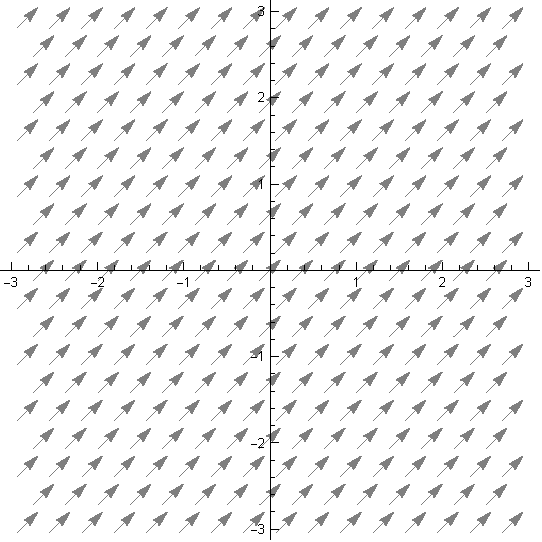
\includegraphics[width=10cm]{images/div0field.pdf}
  \end{center}
  The following field represents $\mathbf{F} = \hat{r}$, which has positive divergence (recall that $\hat{r}$ is not position-independent).
  \begin{center}
    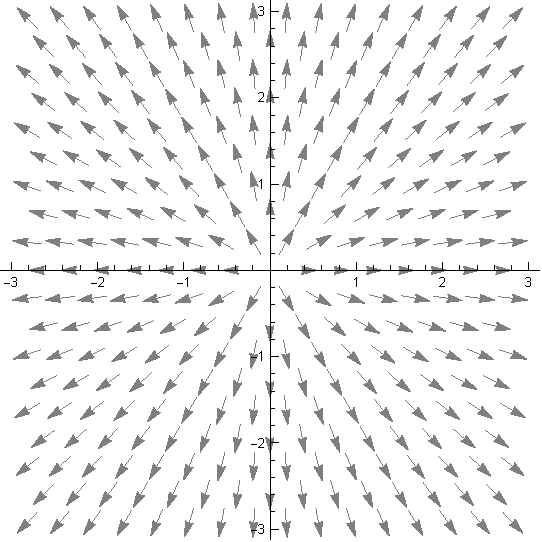
\includegraphics[width=10cm]{images/spreadfield.pdf}
  \end{center}
\end{example}
\begin{definition}[Solenoidal Field]
  A field that has zero divergence is known as a solenoidal or divergence-free field.\newline

  Solenoidal fields are useful for modeling incompressible fluids, as incompressible fluids have constant density.\newline

  If $\nabla \cdot \mathbf{F} = 0$, then $\mathbf{F} = \nabla \times \mathbf{A}$ for some other vector field $\mathbf{A}$. Additionally, since $\mathbf{F} = \nabla \Phi$ for some scalar field $\Phi$, we recover Laplace's equation:
  \begin{align*}
    \nabla\cdot \left(\nabla \Phi\right) &= 0\\
    \nabla^2\Phi &= 0.
  \end{align*}
\end{definition}
\begin{example}[Understanding the Curl]
  Of the nine combinations $\partial_i F_j$, we have used $3$ of them via the divergence.\newline

  Now, we explore the curl, which is $\nabla \times \mathbf{F}$, which gives information about $\partial_iF_j$ where $i \neq j$.\newline

  By the definition of the cross product, we have
  \begin{align*}
    \left(\nabla \times \mathbf{F}\right)_{k} &= \partial_iF_j - \partial_jF_i,
  \end{align*} 
  where $i\neq j$.\newline

  Considering water rotating with angular velocity $\omega$, we find $\mathbf{v} = \omega\times \mathbf{r}$. Now, taking
  \begin{align*}
    \nabla \times \mathbf{v} &= \nabla \times \left(\mathbf{r}\times \omega\right)\\
                             &= 2\omega.
  \end{align*}
  Therefore, curl measures some ``swirl'' of a given vector field.
\end{example}
\begin{example}[Fields with Differing Curl]
  The field $\mathbf{F} = \left(x-y\right)\hat{i} + \left(x+y\right)\hat{j}$ has positive curl everywhere.
  \begin{center}
    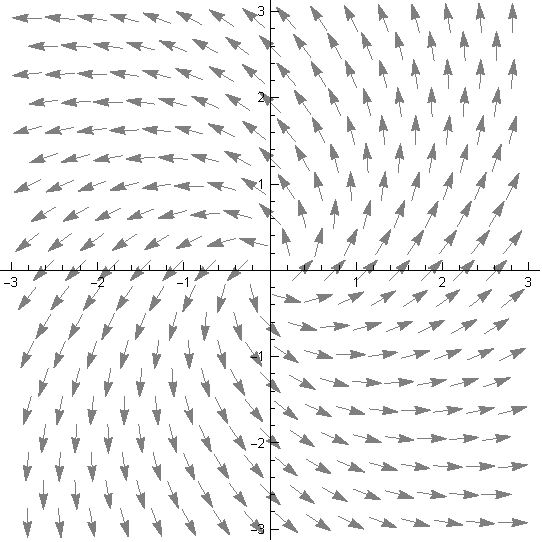
\includegraphics[width=10cm]{images/curl1a.pdf}
  \end{center}
  Meanwhile, the field $\mathbf{F} = \left(x+y\right)\hat{i} + \left(x-y\right)\hat{j}$ has zero curl everywhere.
  \begin{center}
    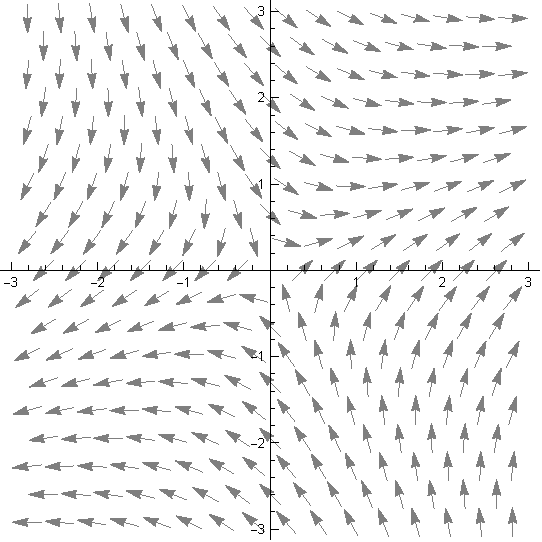
\includegraphics[width=10cm]{images/curl1b.pdf}
  \end{center}
\end{example}
\subsection{Integrating Scalar and Vector Fields}%
\begin{table}
  \centering
  \renewcommand{\arraystretch}{2.5}
  \begin{tabular}{c|c}
    Type of Integral & Expression\\
    \hline\hline
    Line Integral, $C = y(x)$ & $\displaystyle \int_{x_1}^{x_2} f\left(x,g(x)\right)\sqrt{1 + \left(\frac{dy}{dx}\right)^2}\:dx$\\
    Line Integral, $\mathbf{c}(t) = \left(x(t),y(t)\right)$ & $\displaystyle\int_{t_1}^{t_2}f\left(x(t),y(t)\right)\norm{\frac{d\mathbf{c}}{dt}}\:dt$\\
    \hline
    Surface Integral, $z = g(x,y)$ & $\displaystyle \int_{D}^{} f\left(x,y,g(x,y)\right)\sqrt{1 + \norm{\nabla g}^2}\:dxdy$\\
    Surface Integral, $\mathbf{r} = \mathbf{x} (s,t)$ & $\displaystyle \int_{t_1}^{t_2}\int_{s_1}^{s_2} f\left(\mathbf{r}\right)\norm{\pd{\mathbf{x}}{s}\times \pd{\mathbf{x}}{t}}\:dsdt$.
  \end{tabular}
  \caption{Integrating Scalar Fields}
\end{table}
\begin{table}
  \centering
  \renewcommand{\arraystretch}{2}
  \begin{tabular}{c|c}
    Type of Integral & Expression\\
    \hline\hline
    $\int_{C}^{} \mathbf{B}\cdot\:d\vec{\ell}$, $\mathbf{B} = B_x\hat{i} + B_y\hat{j} + B_z\hat{k}$ & $\displaystyle \int_{C} B_x\:dx + B_y\:dy + B_z\:dz$\\
    $\int_{C}^{} \mathbf{B}\cdot\:d\vec{\ell}$, $\mathbf{B} = B_r\hat{r} + B_{\phi}\hat{\phi} + B_z\hat{k}$ & $\displaystyle \int_{C} B_r\:dr + rB_{\phi}\:d\phi + B_z\:dz$\\
    $\int_{C}^{} \mathbf{B}\cdot\:d\vec{\ell}$, $\mathbf{B} = B_r\hat{r} + B_{\phi}\hat{\phi} + B_{\theta}\hat{\theta}$ & $\displaystyle \int_{C} B_{r}\:dr + r\sin\theta B_{\phi}\:d\phi + B_{\theta}\:d\theta$\\
    $\int_{C}^{} \mathbf{E}\cdot\:d\vec{\ell}$, $\mathbf{E} = \nabla \Phi$ & $\displaystyle \Phi\left(t_2\right) - \Phi\left(t_1\right)$\\
    \hline
    $\Phi$ & $\displaystyle \int_{S}\mathbf{E}\cdot d\mathbf{a}$\\
    $\Phi_{\text{net}}$ & $\displaystyle \oint_{S}\mathbf{E}\cdot d\mathbf{a}$
  \end{tabular}
  \caption{Integrating Vector Fields}
\end{table}
Integration is summation,\footnote{kinda} meaning the expression
\begin{align*}
  \int_{x_1}^{x_2} f(x)\:dx
\end{align*}
describes a sum along a unique interval defined by $x_1$ and $x_2$.\newline

When we go to higher dimensions, we first think of
\begin{align*}
  \int_{P_1}^{P_2} f(x,y)\:dx,
\end{align*}
which wants us to sum $f(x,y)$ from $P_1 = \left(x_1,y_1\right)$ to $P_2 = \left(x_2,y_2\right)$. However, this is not a fully specific expression --- we need a \textit{path} along which we integrate. We specify the path by $y = g(x)$. Now, the integral becomes
\begin{align*}
  \int_{P_1}^{P_2} f\left(x,g(x)\right)\:dx.
\end{align*}
Similarly, for a surface integral
\begin{align*}
  \int_{S}^{} f(x,y)\:dx dy,
\end{align*}
we need the surface $S$ along which we integrate, where we say $z = g(x,y)$.\newline

However, while there are certain functions that are path-independent,\footnote{Holomorphic functions, for instance} we must assume that every function is path-\textit{dependent}.
\subsubsection{Line Integrals}%
A line integral is a sum over a curve $C$.
\begin{align*}
  \int_{C}^{} f\left(\mathbf{r}\right)\:d\ell.
\end{align*}
Here, $d\ell$ denotes the length element along $C$. For instance, if $f$ denotes the charge density per unit length, and $C$ is a wire, then $\int_{C}^{} f\left(\mathbf{r}\right)\:d\ell$.\newline

If we define $C$ by $y = g(x)$, then the integral is
\begin{align*}
  \int_{C}^{} f(x,y)\:d\ell &= \int_{C}^{} f\left(x,g(x)\right)\:d\ell.
\end{align*}
However, we need to figure out how to deal with $d\ell$ --- in particular, we need $d\ell$ to be an expression only in $dx$. In particular, $d\ell$ is given by the Pythagorean theorem:
\begin{align*}
  \left(d\ell\right)^2 &= \left(dx\right)^2 + \left(dy\right)^2.
\end{align*}
\begin{notation}
  Everyone (else) drops the parentheses:
  \begin{align*}
    d\ell^2 &= dx^2 + dy^2.
  \end{align*}
\end{notation}
Our integral now becomes
\begin{align*}
  \int_{C}^{} f\left(x,g(x)\right)\:d\ell &= \int_{C}^{} f\left(x,g(x)\right)\:\sqrt{\left(dx\right)^2 + \left(dy\right)^2}\\
                                          &= \int_{x_1}^{x_2} f\left(x,g(x)\right)\:dx\sqrt{1 + \left(\frac{dy}{dx}\right)^2}
\end{align*}
\begin{example}
  Let
  \begin{align*}
    f\left(\mathbf{r}\right) &= \sqrt{\frac{1}{4}x^2 + y^2}\\
    y(x) &= \frac{1}{2}x^2,
  \end{align*}
  integrated from $0 < x < 1$.\newline

  Then,
  \begin{align*}
    \int_{C}^{} f\left(\mathbf{r}\right)\:d\ell &= \int_{0}^{1} \sqrt{\frac{1}{4}x^2 + \frac{1}{4}x^4}\sqrt{1 + \left(\frac{dy}{dx}\right)^2}\:dx\\
                                                &= \frac{1}{2}\int_{0}^{1} x\sqrt{1 + x^2}\sqrt{1 + x^2}\:dx\\
                                                &= \frac{1}{2}\int_{0}^{1} x\left(1 + x^2\right)\:dx\\
                                                &= \frac{3}{8}.
  \end{align*}
  Note that we can also evaluate this integral as a function of $y$, and still get the same outcome.
\end{example}
\begin{example}
  Let
  \begin{align*}
    f\left(\mathbf{r}\right) &= \sqrt{\frac{1}{4}x^2 + y^2}\\
    y(x) &= x,
  \end{align*}
  integrated from $0 < x < 1$.\newline

  Then,
  \begin{align*}
    \int_{C}^{} f\left(\mathbf{r}\right)\:d\ell &= \int_{0}^{1} \sqrt{\frac{1}{4}x^2 + x^2}\sqrt{1 + \left(\frac{dy}{dx}\right)^2}\:dx\\
                                                &= \sqrt{\frac{5}{2}}\int_{0}^{1} x\:dx\\
                                                &= \sqrt{\frac{5}{8}}.
  \end{align*}
  We can also do this in polar coordinates. First, we have
  \begin{align*}
    \left(d\ell\right)^2 &= \left(dr\right)^2 + r^2\left(d\theta\right)^2.
  \end{align*}
  Then,
  \begin{align*}
    \int_{C}^{} f\left(\mathbf{r}\right)\:d\ell &= \int_{0}^{\sqrt{2}} \sqrt{\frac{1}{4}r^2\cos^2\theta + r^2\sin^2\theta}\:dr\\
                                                &= \sqrt{\frac{5}{8}}.
  \end{align*}
\end{example}
When we integrate with respect to a parametrized curve in one dimension, we have
\begin{align*}
  \int_{x_1}^{x_2} f(x)\:dx &= \int_{t(x_1)}^{t(x_2)} f\left(x(t)\right)\frac{dx}{dt}\:dt.
\end{align*}
In multiple dimensions for $c(t) = \left(x(t),y(t)\right)$, we have
\begin{align*}
  d\ell &= \sqrt{\left(dx\right)^2 + \left(dy\right)^2}\\
        &= dt\sqrt{\left(\frac{dx}{dt}\right)^2 + \left(\frac{dy}{dt}\right)^2}\\
        &= \norm{\frac{d\mathbf{c}}{dt}},
\end{align*}
yielding
\begin{align*}
  \int_{C}^{} f\left(\mathbf{r}\right)\:d\ell &= \int_{t_1}^{t_2} f(x(t),y(t))\norm{\frac{d\mathbf{c}}{dt}}\:dt.
\end{align*}
\subsubsection{Surface Integrals}%
When we turn to a surface
\begin{align*}
  \int_{S}^{} f\left(\mathbf{r}\right)\:dA,
\end{align*}
we parametrize $z = g(x,y)$ to yield
\begin{align*}
  \int_{S}^{} f\left(x,y,z\right)\:dA &= \int_{D}^{} f\left(x,y,g(x,y)\right)\sqrt{1 + \norm{\nabla g}^2}\:dx dy,
\end{align*}
where $D$ is the projection of $S$ onto the $x,y$-plane.
\subsubsection{Circulation}%
So far, we have only considered scalar  fields, When we look at
\begin{align*}
  \int_{C}^{} \mathbf{F}\left(\mathbf{r}\right)\:d\ell &= \hat{i}\int_{C}^{} F_x\left(\mathbf{r}\right)\:d\ell + \hat{j}\int_{C}^{} F_y\left(\mathbf{r}\right)\:d\ell + \hat{k}\int_{C}^{} F_z\left(\mathbf{r}\right)\:d\ell.
\end{align*}
More commonly, though, we are interested in
\begin{align*}
  \int_{C}^{} \mathbf{F}\left(\mathbf{r}\right)\cdot\:d\vec{\ell},
\end{align*}
which is a scalar quantity. When we add the dot product into the integral, we signal that we are most interested in the \textit{parallel} component of $\mathbf{F}$ to $d\vec{\ell}$.\newline

In cartesian coordinates, this integral is equal to
\begin{align*}
  \int_{C}^{} \mathbf{F}\left(\mathbf{r}\right)\cdot\:d\vec{\ell} &= \int_{C}^{}F_x dx + F_y dy + F_z dz.
\end{align*}
For a more physical example,\footnote{Who cares about that?} this integral is a measure of work if $\mathbf{F}\left(\mathbf{r}\right)$ denotes force. Similarly,
\begin{align*}
  \Delta V &= -\int_{P_1}^{P_2} \mathbf{E}\cdot\:d\vec{\ell}
\end{align*}
\begin{definition}[Circulation]
When we integrate over a closed curve $C$, our line integral now becomes
\begin{align*}
  \Psi &= \oint_{C}^{} \mathbf{F}\cdot \:d\vec{\ell}
\end{align*}
\end{definition}
\begin{remark}
  It is not always the case that $\Psi$ is zero.
\end{remark}
Summing $\mathbf{F}$ along a closed path $C$ measures the net ``swirl'' of the vector field.
\begin{example}[Symmetry in Circulation]
  Ampère's law says that
  \begin{align*}
    \oint_{C}^{} \mathbf{B}\cdot \:d\vec{\ell} &= \mu_0 I,
  \end{align*}
  where $\mu_0$ is the permeability of free space, $I$ denotes current, and $\mathbf{B}$ is the magnetic field.\newline

  Consider the case of a wire with constant radius $a$ and uniform current $I_0$. From cylindrical symmetry, it must be the case that $\mathbf{B}$ forms concentric circles about the wire.\newline

  Since Ampère's law says we can \textit{always} pick a curve that yields a constant, we can let $C$ correspond to one of the circles with constant $\norm{\mathbf{B}}$.
  \begin{align*}
    \oint_{C}^{} \mathbf{B}\cdot\:d\vec{\ell} &= \oint_{C}^{} B\:d\ell\\
                                             &= B\oint_{C}^{} \:d\ell\\
                                             &= 2\pi r B,
  \end{align*}
  where $r$ is the radius of the loop $C$.\newline

  Note that this value does not depend on the radius of $C$, but the value of $\mu_0 I$ does depend on the radius of $C$.\newline

  In particular,
  \begin{align*}
    I\left(r < a\right) &= I_0\frac{r^2}{a^2},
  \end{align*}
  yielding
  \begin{align*}
    \mathbf{B}\left(r < a\right) &= \frac{\mu_0 I_0}{2\pi}\frac{r}{a^2}\hat{\phi}\\
    \mathbf{B}\left(r > a\right) &= \frac{\mu_0I_0}{2\pi r} \hat{\phi}.
  \end{align*}
  Inside the wire, the magnitude of the $B$ field grows linearly with respect to $r$, and outside, the magnitude of the $B$ field falls off by a factor of $r^{-1}$.
\end{example}
However, in the general case, we need to parametrize our line integral.
\begin{align*}
  \int_{C}^{} \mathbf{F}\cdot\:d\vec{\ell} &= \int_{t_1}^{dt} \left(\mathbf{F}\cdot \frac{d\mathbf{c}}{dt}\right)\:dt
\end{align*}
\begin{example}[Path-Dependence (or Path-Independence) of Work]
  Let $\mathbf{B} = x^2y\hat{i} - xy^2\hat{j}$, $P_1 = (0,0)$, and $P_2 = (1,1)$. We will calculate the work done by $\mathbf{B}$ as follows:
  \begin{align*}
    \int_{C}^{} \mathbf{B}\cdot\:d\vec{\ell} &= \int_{C}^{} B_x\:dx + B_y\:dy.
  \end{align*}
  Along the path $C_1$, which goes from $(0,0)$ to $(1,0)$, then $(1,0)$ to $(1,1)$, the work is given by
  \begin{align*}
    \int_{C}^{} \mathbf{B}\cdot\:d\vec{\ell} &= \int_{C_1}^{} x^2y\:dx-xy^2\:dy
                                             &= \int_{0}^{1} x^2y\bigr\vert_{y=0}\:dx - \int_{0}^{1} xy^2\bigr\vert_{x=1}\:dy\\
                                             &= -\frac{1}{3}.
  \end{align*}
  Along the path $C_2$, which goes from $(0,0)$ to $(1,1)$ directly, with $x = y$ and $dy = dx$, we have
  \begin{align*}
    \int_{C_2}^{} \mathbf{B}\cdot\:d\vec{\ell} &= \int_{C_2}^{} \left(x^2y-xy^2\right)\bigr\vert_{y=x}\:dx\\
                                               &= 0.
  \end{align*}
  Along the path $C_3$, defined by $x = 1-\cos\theta$ and $y = \sin\theta$, we have $\left(dx,dy\right) = \left(\sin\theta,\cos\theta\right)d\theta$, meaning
  \begin{align*}
    \int_{C_3}^{} \mathbf{B}\cdot\:d\vec{\ell} &= \int_{0}^{\pi/2} \left(\left(1-\cos\theta\right)^2\sin\theta\right)\sin\theta\:d\theta - \int_{0}^{\pi/2} \left(\left(1-\cos\theta\right)\sin^2\theta\right)\cos\theta\:d\theta\\
                                               &= \frac{3\pi}{8}-1.
  \end{align*}
  Meanwhile, for $\mathbf{E} = xy^2\hat{i} + x^2y\hat{j}$, it is the case that
  \begin{align*}
    \int_{C_1}^{} \mathbf{E}\cdot\:d\vec{\ell} &= \frac{1}{2}\\
    \int_{C_2}^{} \mathbf{E}\cdot\:d\vec{\ell} &= \frac{1}{2}\\
    \int_{C_3}^{} \mathbf{E}\cdot\:d\vec{\ell} &= \frac{1}{2}.
  \end{align*}
\end{example}
\begin{definition}[Path-Independence]
  Let $\mathbf{F}\left(\mathbf{r}\right)$ be a vector field. If, for every closed path $C$, it is the case that
  \begin{align*}
    \oint_{C}^{} \mathbf{F}\cdot\:d\vec{\ell} &= 0,
  \end{align*}
  then we say $\mathbf{F}$ is path-independent.
\end{definition}
If our vector field is path-independent, then we are allowed to pick the path that is easiest to calculate.\newline

If $\mathbf{E}$ is path-independent, then there has to exist some scalar field $\Phi$ such that
\begin{align*}
  \int_{t_1}^{t_2} \mathbf{E}\cdot\:d\vec{\ell} &= \Phi\left(t_2\right)- \Phi\left(t_1\right)
\end{align*}
\begin{definition}[Equivalent Conditions for Path-Independence]
Let $\mathbf{F}\left(\mathbf{r}\right)$ be a vector field. Then, the following are equivalent:
\begin{itemize}
  \item $\displaystyle \oint\int_{C}^{} \mathbf{F}\cdot\:d\vec{\ell} = 0$
  \item $\mathbf{F} = \nabla \Phi$
  \item $\nabla \times \mathbf{F}=0$
\end{itemize}
\end{definition}
\begin{example}[Finding the Scalar Field]
  Consider $\mathbf{E} = xy^2\hat{i} + x^2y\hat{j}$. Since $\mathbf{E}$ has curl $0$, we know there must exist some $\Phi$ such that
  \begin{align*}
    \pd{\Phi}{x} &= xy^2\\
    \Phi &= \frac{1}{2}x^2y^2 + f(y)\\
    \pd{\Phi}{y} &= x^y\\
    \Phi &= \frac{1}{2}x^2y^2 + g(x).
  \end{align*}
  Such a $\Phi$ exists if and only if we can choose $f$ and $g$ to be the same function. Since we can set $f(y) = g(x) = c\in \R$, such a $\Phi$ exists --- namely, $\Phi(x,y) = \frac{1}{2}x^2y^2$.\newline

  Consider $\mathbf{B} = x^2y\hat{i} = xy^2\hat{j}$. We know such a $\Phi$ must not exist.
  \begin{align*}
    \pd{\Phi}{x} &= x^2y\\
    \Phi &= \frac{1}{3}x^3y + f(y)\\
    \pd{\Phi}{y} &= -xy^2\\
    \Phi &= -\frac{1}{3}xy^3 + g(x).
  \end{align*}
  There cannot exist such $f$ and $g$ that makes these antiderivatives equal to each other.
\end{example}
\begin{example}[Gravity]
  A mass $m$ has a gravitational field
  \begin{align*}
    \mathbf{g} &= -Gm\frac{\hat{r}}{r^2}.
  \end{align*}
  Conventionally, the gravitational potential is the negative of the line integral of $\mathbf{g}$, since we want $\Phi\left(\infty\right) = 0$, yielding
  \begin{align*}
    \Phi\left(r\right) &= -\int_{\infty}^{r} \mathbf{g}\cdot\:d\vec{\ell}\\
                       &= Gm\int_{\infty}^{r} \frac{1}{s^2}\:ds\\
                       &= -\frac{Gm}{r}.
  \end{align*}
  Consider a planet. A planet is a bunch of point masses, which means we orient our focus away from $\mathbf{g}$ towards $d\mathbf{g}$, and $m$ to $dm = \rho d\tau$.\newline

  However, instead of trying to work out this integral in vector form, we want to find a scalar field $\Phi$, then take $\mathbf{g} = -\nabla \Phi$.\newline

  Let's construct a planet that is a spherical shell at radius $a$ with mass $m$. Then, $\sigma = \frac{m}{4\pi a^2}$ (constant), with the area $dA$ has mass $dm = \sigma dA$. Thus, the mass at distance $\mathbf{r}$ is
  \begin{align*}
    d\mathbf{g} &= -G\frac{\left(\mathbf{r} - \mathbf{s}\right)}{\norm{\mathbf{r} - \mathbf{s}}^3} \sigma dA.
  \end{align*}
  To find the total gravitational field, we find
  \begin{align*}
    \mathbf{g}\left(\mathbf{r}\right) &= -G\int_{S}^{} \frac{\mathbf{r} - \mathbf{s}}{\norm{\mathbf{r} - \mathbf{s}}^3}\sigma\:dA,
  \end{align*}
  where the integral with respect to $\mathbf{s}$ is over the surface.\newline

  This vector-valued integral kind of sucks,\footnote{Citation needed.} so instead, we want to integrate
  \begin{align*}
    \Phi\left(\mathbf{r}\right) &= -G\int_{S}^{} \frac{1}{\norm{\mathbf{r} - \mathbf{s}}}\sigma\:dA,
  \end{align*}
  which is much easier to do. Notice that
  \begin{align*}
    \norm{\mathbf{r} - \mathbf{s}}^2 &= \iprod{\mathbf{r}-\mathbf{s}}{\mathbf{r}-\mathbf{s}}\\
                                     &= \norm{\mathbf{r}}^2 + \norm{\mathbf{s}}^2 - 2\norm{\mathbf{r}}\norm{\mathbf{s}}\cos\theta,
  \end{align*}
  meaning, with $\norm{\mathbf{r}} = r$ and $\norm{\mathbf{s}} = a$,
  \begin{align*}
    \norm{\mathbf{r} - \mathbf{s}} &= \sqrt{r^2 + a^2 - 2ra\cos\theta}.
  \end{align*}
  Using the area element, $dA = a^2d\Omega$, or $dA = 2\pi a^2d\left(\cos\theta\right)$, we get
  \begin{align*}
    \Phi\left(\mathbf{r}\right) &= -2\pi G\sigma a^2\int_{-1}^{1} \frac{1}{\sqrt{r^2 + a^2 - 2ra\cos\theta}}\:d\left(\cos\theta\right)\\
                                &= \frac{-2\pi G\sigma a}{r}\left(\left(r + a\right) - \left\vert r-a \right\vert\right).
  \end{align*}
  We need to evaluate $\Phi$ for $r < a$ and for $r > a$.
  \begin{align*}
    \Phi\left(r < a\right) &= -4\pi G\sigma a\\
                           &= -\frac{Gm}{a}\\
    \Phi\left(r > a\right) &= -\frac{4\Pi G\sigma a^2}{r}\\
                           &= -\frac{Gm}{r}.
  \end{align*}
  Notice that inside the shell, the gravitational potential is constant, while outside the shell, the gravitational potential falls off as if the shell has its mass concentrated at a point in the center.\newline

  When we convert the spherical shell into a ball (by integrating over $a$), we can see that, outside the planet, it is still the case that gravitational potential depends solely on the distance to the center of the sphere.
\end{example}
\subsubsection{Flux}%
While circulation is the measure of the ``swirl'' of a vector field about a curve, we are also interested in the ``surge'' of a vector field about a surface. This is what flux is.
\begin{definition}[Flux]
The flux is the product of the field's magnitude and surface area $A$ that it crosses.
\begin{align*}
  \Phi \equiv EA.
\end{align*}
A surface is identified with its orientation, $\hat{n}$, meaning
\begin{align*}
  \Phi &= \mathbf{E}\cdot \hat{n} A.
\end{align*}
If $\hat{n}$ is not constant along a curve's surface, flux is calculated with an integral.
\begin{align*}
  \Phi &= \int_{S}^{} \mathbf{E}\cdot \hat{n}\:da\\
       &= \int_{S}^{} \mathbf{E}\cdot d\mathbf{a}.
\end{align*}
If $S$ is a closed surface,\footnote{A surface with no boundary.} the flux is known as the net flux, and is denoted
\begin{align*}
  \Phi_{\text{net}} &= \oint_{S}^{} \mathbf{E}\cdot d\mathbf{a}.
\end{align*}
\end{definition}
\begin{example}[Continuity Equation]
  The conservation of electric charge is expressed by continuity --- the rate at which charge is lost in a surface, $Q_{\text{in}}$ must be accounted for by the current flowing out of the surface, $I_{\text{out}}$.
  \begin{align*}
    I_{\text{out}} &= -\frac{dQ_{\text{in}}}{dt}.
  \end{align*}
  We define the charge density $\rho$ as
  \begin{align*}
    Q_{\text{in}} &= \int_{V}^{} \rho\:d\tau,
  \end{align*}
  and the movement of charge density with average drift velocity $\mathbf{v}$ gives the current density, $\mathbf{J} = \rho \mathbf{v}$. Since $\mathbf{J}$ has units of current per area, the usual current is measured by
  \begin{align*}
    I &= \int_{S}^{} \mathbf{J}\cdot d\mathbf{a}.
  \end{align*}
  In particular, continuity is concerned with net flux, meaning
  \begin{align*}
    I_{\text{out}} &= \oint_{S}^{} \mathbf{J} \cdot d\mathbf{a},
  \end{align*}
  so the continuity equation is
  \begin{align*}
    \oint_{S}^{} \mathbf{J}\cdot d\mathbf{a} &= -\frac{d}{dt}\int_{V}^{} \rho\:d\tau,
  \end{align*}
  where $S$ bounds the volume $V$.
\end{example}
\begin{example}[Gauss's Law]
  Gauss's Law states that the net flux about an enclosed surface is proportional to the charge enclosed.
  \begin{align*}
    \oint_{S}^{} \mathbf{E}\cdot d\mathbf{a} &= \frac{q_{\text{encl}}}{\epsilon_{0}}.
  \end{align*}
  We would find it weird to find $\mathbf{E}$ using Gauss's law, unless the symmetry works heavily in our favor.\newline

  Consider a uniform ball with positive charge $Q_0$ and radius $a$. Since the charge is spherically symmetric, $\mathbf{E}$ must be radial, implying $\mathbf{E} = E(r)\hat{r}$.\newline

  With this in mind, we can choose a surface $S$ such that $\mathbf{E}$ is parallel to $d\mathbf{a} = \hat{n} da$,\footnote{For a sphere, $\hat{n} = \hat{r}$} and of constant magnitude on $S$.\newline

  For $r > a$, our enclosed charge is
  \begin{align*}
    \oint_{S}\mathbf{E}\cdot d\mathbf{a} &= \oint_{S}E(r)\hat{r}\cdot \hat{r}\:da\\
                                         &= E(r)\oint_{S}\:da\\
                                         &= 4\pi r^2 E(r)\\
                                         &= \sigma 4\pi a^2\\
    E &= \frac{Q_0}{4\pi \epsilon r^2}\\
    \mathbf{E} &= \frac{Q_0}{4\pi \epsilon_0 r^2}\hat{r}.
  \end{align*}
  If our Gaussian surface is inside the sphere, then with our charge density $\rho = \frac{Q_0}{4/3 \pi a^3}$, implying
  \begin{align*}
    q_{\text{encl}} &= \rho \frac{4}{3}\pi r^3\\
                    &= Q_0\frac{r^3}{a^3}.
  \end{align*}
  Thus, inside the ball, we get
  \begin{align*}
    \mathbf{E} &= \frac{Q_0}{4\pi \epsilon_0}\frac{r}{a^3}\hat{r}.
  \end{align*}
\end{example}
\begin{recall}
  A vector field $\mathbf{E}$ is path independent if
  \begin{align*}
    \oint_{C} \mathbf{E}\cdot d\vec{\ell} &= 0\\
    \mathbf{E} &= \nabla \Phi\\
    \nabla \times \mathbf{E} &= 0.
  \end{align*}
  This is also known as an irrotational vector field.
\end{recall}
\begin{example}[Surface Independence]
  Let $\mathbf{E} = xy^2\hat{i} + x^2y\hat{j}$ and $\mathbf{B} = x^2y\hat{i} - xy^2\hat{j}$. We will examine the flux of these fields about different surfaces.
  \begin{example}[Flux of $\mathbf{E}$ about $S_1$]
    We define $S_1$ to be a quarter circle of radius $a$ in the $yz$-plane, defined at $x=b$. To define $d\mathbf{a}$, we define the orientation to be in the $\hat{i}$ direction, meaning $d\mathbf{a} = \hat{i}\:dydz$. Our integral becomes
    \begin{align*}
      \int_{S_1}^{} \mathbf{E}\cdot d\mathbf{a} &= \int_{S_1}^{} xy^2\:dydz.
    \end{align*}
    We don't want to do this integral in cartesian coordinates, so we do a change of coordinates
    \begin{align*}
      \int_{S_1}^{} \mathbf{E}\cdot d\mathbf{a} &= \int_{S_1}^{} xy^2\:dydz\\
                                                &= \int_{S_1}^{} xy^2 r\:dr d\phi,\\
                                                &= b\int_{S_1}^{} y^2\:dr d\phi\\
                                                &= b\int_{0}^{a}r^3\:dr\int_{0}^{\pi/2}\cos^2\phi\:d\phi\\
                                                &=\frac{\pi}{16}a^4b.
    \end{align*}
  \end{example}
  \begin{example}[Flux of $\mathbf{E}$ about $S_2$]
    Let $S_2$ be a quarter cylinder of radius $a$ in the $yz$-plane, with $b < x < 2b$. We are integrating over four faces --- the rectangle in the $xz$-plane, the rectangle in the $xy$-plane, the quarter-circle at $x = 2b$ in the $yz$-plane, and the radial face between $x=b$ and $x=2b$.\newline

    The rectangle in the $xy$-plane has its orientation in the $-\hat{k}$ direction, meaning $\mathbf{E}\cdot d\mathbf{a}_1 = 0$, and similarly, the rectangle in the $xz$-plane has its orientation in the $-\hat{j}$ direction, meaning $\mathbf{E}\cdot d\mathbf{a}_2 = 0$. The quarter circle cap at $x=2b$ has its orientation in the positive $x$ direction --- in cylindrical coordinates, this becomes $d\mathbf{a}_3 = \hat{i}\:\rho\:d\rho d\phi$. On the radial face, we have $d\mathbf{a}_4 = \hat{\rho} a\:d\phi dx$.
    \begin{align*}
      \int_{S_2}^{} \mathbf{E}\cdot d\mathbf{a} &= \sum_{i}\int_{s_i}^{} \mathbf{E}\cdot d\mathbf{a}_i\\
                                                &= 0 + 0 + \int_{s_3}^{} xy^2\rho\:d\rho d\phi + \int_{s_4}^{} \mathbf{E}\cdot \hat{\rho}\:d\phi dx\\
                                                &= \frac{\pi}{8}a^2 b\left(a^2 + \frac{14}{3}b^2\right).
    \end{align*}
  \end{example}
  Note that in our previous two examples, the surface affected the flux.
  \begin{example}[Flux of $\mathbf{B}$ about $S_1$]
    \begin{align*}
      \int_{S_1}^{} \mathbf{B}\cdot d\mathbf{a} &= \frac{1}{3}a^3b^2
    \end{align*}
  \end{example}
  \begin{example}[Flux of $\mathbf{B}$ about $S_2$]
    \begin{align*}
      \int_{S_2}^{} \mathbf{B}\cdot d\mathbf{a} &= \int_{s_3}^{} xy^2\rho\:d\rho d\phi + \int_{s_4}^{} \mathbf{B}\cdot \hat{\rho} a\:d\phi dx\\
                                                &= \frac{1}{3}a^3b^2.
    \end{align*}
  \end{example}
  In this case, we can see that $\mathbf{B}$ has the same flux integral. Later, we will see that $\mathbf{B}$ is ``surface independent,'' in the sense that since both $S_1$ and $S_2$ have the same boundary, the flux integral of $\mathbf{B}$ only depends on the boundary.
\end{example}
\begin{definition}[Surface Independence]
  Let $\mathbf{B}$ be a vector field. If, for any closed surface $S$,
  \begin{align*}
    \oint_{S}\mathbf{B}\cdot d\mathbf{a} &= 0,
  \end{align*}
  then we say $\mathbf{B}$ is surface independent.
\end{definition}
For a surface-independent field, the integral about an arbitrary surface must be the same same through any surface bounded by the same closed curve, implying the existence of a vector potential $\mathbf{A}$ such that
\begin{align*}
  \int_{S}^{} \mathbf{B}\cdot d\mathbf{a} &= \oint_{C}\mathbf{A}\cdot d\vec{\ell},
\end{align*}
where $C$ is the boundary of $S$ --- note that this equivalence only holds with respect to a particular orientation. By convention, we use the positive orientation on $C$, which implies that $\hat{n}$ has outward orientation on $S$.\newline

Since $\mathbf{A}$ is a vector potential, we can yield another field $\mathbf{F} = \nabla \times \mathbf{A}$. Thus, we get Stokes's Theorem
\begin{align*}
  \int_{S}^{} \nabla \times \mathbf{A}\cdot d\mathbf{a} &= \oint_{C}\mathbf{A}\cdot d\vec{\ell}.
\end{align*}
Notice that the divergence of a curl is zero, so we can see that $\nabla \cdot \mathbf{F} = 0$.
\begin{definition}[Three Equivalent Criteria for Surface Independence]
  Let $\mathbf{F}$ be a surface independent vector field. Then, the following are equivalent:
  \begin{align*}
    \oint_{S}F\cdot d\mathbf{a} &= 0\\
    \mathbf{F} &= \nabla \times \mathbf{A}\\
    \nabla \cdot \mathbf{F} &= 0.
  \end{align*}
\end{definition}
\begin{example}[Finding $\mathbf{A}$]
  Let $\mathbf{B}$ be such that $\nabla \mathbf{A} = \mathbf{B}$. Then,
  \begin{align*}
    \mathbf{B} &= \begin{cases}
      x^2y = \partial_y A_z - \partial_z A_y\\
      -xy^2 = \partial_z A_x - \partial_x A_z\\
      0 = \partial_x A_y - \partial_y A_x
    \end{cases}.
  \end{align*}
  If we let $A_x = A_y = 0$, then we solve the equation by taking
  \begin{align*}
    x^2 y &= \partial_y A_z\\
    xy^2 &= \partial_xA_z,
  \end{align*}
  yielding
  \begin{align*}
    A_z &= \frac{1}{2}x^2y^2 + \alpha(x,z)\\
    A_z &= \frac{1}{2}x^2y^2 + \beta(y,z).
  \end{align*}
  For consistency, it must be the case that $\alpha(x,z) = \beta(y,z) = \gamma(z)$. Thus, we get
  \begin{align*}
    \mathbf{A}_1 &= \left(\frac{1}{2}x^2y^2 + \gamma(z)\right)\hat{k}.
  \end{align*}
  We can also find
  \begin{align*}
    \mathbf{A}_2 &= \left(-xy^2z + \beta(x,y)\right)\hat{i} + \left(-x^2yz + \alpha(x,y)\right)\hat{j},
  \end{align*}
  whose curl is also $\mathbf{B}$.\newline

  Note that this means $\mathbf{A}$ it not unique. In particular, for any $\mathbf{A}$, we can add any gradient field $\nabla \chi$, since $\nabla \times \nabla \chi = 0$.
\end{example}
\subsection{Calculating Flux Integrals with Boundary Geometry}%
\begin{table}
  \renewcommand{\arraystretch}{2}
  \centering
  \begin{tabular}{c|c}
    Theorem & Expression\\
    \hline\hline
    Divergence Theorem & $\displaystyle \int_{V}^{} \nabla \cdot \mathbf{E}\:d\tau = \oint_{\partial V}^{} \mathbf{E}\cdot d\mathbf{a}$\\
    Divergence Theorem, Gradients & $\displaystyle \int_{V}^{} \nabla \Phi\:d\tau = \oint_{\partial V}^{} \Phi d\mathbf{a}$\\
    Divergence Theorem, Curls & $\displaystyle \int_{V}^{} \nabla \times \mathbf{E}\:d\tau = \oint_{\partial V}^{} \:d\mathbf{a}\times \mathbf{E}$\\
    \hline
    Green's Theorem & $\displaystyle \int_{C}^{} \mathbf{B}\cdot d\vec{\ell} = \int_{S}^{} \left(\pd{B_y}{x} - \pd{B_x}{y}\right)\:dxdy$\\
    Stokes's Theorem & $\displaystyle \int_{S}^{} \nabla \times \mathbf{B}\:d\mathbf{a} = \int_{\partial S}^{} \mathbf{B}\cdot d\vec{\ell}$\\
    Stokes's Theorem, Gradients & $\displaystyle \oint_{C}\Phi d\vec{\ell} = \int_{S}d\mathbf{a}\times \nabla \Phi$\\
    Stokes's Theorem, Curls & $\displaystyle \oint_{C}d\vec{\ell}\times \mathbf{E} = \int_{S}\left(d\mathbf{a}\times \nabla\right)\times \mathbf{E}$
  \end{tabular}
  \caption{Generalized Stokes's Theorem}
\end{table}
Recall the fundamental theorem of calculus:
\begin{align*}
  \int_{a}^{b} \frac{df}{dx}\:dx &= f(b) - f(a).
\end{align*}
In higher dimensions along a path $C$ traveling from $\mathbf{r}_1$ to $\mathbf{r}_2$, we have
\begin{align*}
  \int_{C}^{} \nabla f\cdot d\vec{\ell} &= f\left(\mathbf{r}_2\right) - f\left(\mathbf{r}_1\right).
\end{align*}
Notice that, via this process, we convert from a local property (derivatives) to a property defined by the boundary of a region (in this case, the endpoints of an interval and/or curve).
\subsubsection{Divergence Theorem}%
Consider an infinitesimal box with length $dx$, height $dy$, and depth $dz$. We can see that the flux of $\mathbf{E}$ about these faces is
\begin{align*}
  d\Phi_{\text{net}} &= \sum_{i}\mathbf{E}\cdot d\mathbf{a}_i.
\end{align*}
Evaluating $\mathbf{E}$ at the faces on the $yz$ plane parallel to the $x$ axis, we get
\begin{align*}
  \mathbf{E}\left(0,0,0\right)\cdot d\mathbf{a}_{\text{left}} + \mathbf{E}\left(dx,0,0\right)\cdot d\mathbf{a}_{\text{right}} &= -E_x(0,0,0)dydz + E_x\left(dx,0,0\right)dydz.
\end{align*}
The x component of $d\Phi_{\text{net}}$ is, thus,
\begin{align*}
  d\phi_{1} &- \left(E_x\left(dx,0,0\right)- E_x(0,0,0)\right)dydz\\
            &= \left(\pd{E_x}{x}dx\right)dydz.
\end{align*}
Similarly,
\begin{align*}
  d\phi_2 &= \left(\pd{E_y}{y}dy\right)dzdx\\
  d\phi_3 &= \left(\pd{E_z}{z}dz\right)dxdy.
\end{align*}
Therefore, 
\begin{align*}
  d\Phi_{\text{net}} &= \left(\pd{E_x}{x}dx\right)dydz + \left(\pd{E_y}{y}dy\right)dzdx + \left(\pd{E_z}{z}dz\right)dxdy\\
                     &= \left(\nabla \cdot \mathbf{E}\right)d\tau,
\end{align*}
where $d\tau = dxdydz$ is the volume element. Thus, we see that the infinitesimal flux is proportional to the divergence of $\mathbf{E}$.\newline

To convert from infinitesimal boxes to a full (bounded) region, we cut up $V$ into a bunch of small boxes. The interior box faces' respective fluxes cancel each other out since they have opposite-facing normals.
\begin{theorem}
    Let $V$ be a compact surface in $\R^3$ with piecewise smooth boundary $\partial V$, and $\mathbf{E}$ a continuously differentiable vector field defined on a neighborhood of $V$. Then, the following is true
  \begin{align*}
    \int_{V}^{} \nabla \cdot \mathbf{E}\:d\tau &= \oint_{\partial V}^{} \mathbf{E}\cdot d\mathbf{a}.
  \end{align*}
\end{theorem}
\begin{example}
  Let $\mathbf{E} = r^{\alpha}\hat{r}$, and $V$ be a sphere of radius $R$. Since we have spherical symmetry, we can find the flux of $\mathbf{E}$ about the sphere by taking
  \begin{align*}
    \oint_{S}\mathbf{E}\cdot d\mathbf{a} &= \oint r^{\alpha}R^2d\Omega\\
                                         &= 4\pi R^{\alpha + 2}.
  \end{align*}
  Using the divergence theorem, we take $\nabla \cdot \mathbf{E} = \frac{1}{r^2}\pd{}{r}\left(r^2E_{r}\right) = \left(\alpha + 2\right)r^{\alpha - 1}$, and take
  \begin{align*}
    \int_{V}^{} \nabla \cdot \mathbf{E}\:d\tau &= \left(\alpha + 2\right)\int_{0}^{R} r^{\alpha - 1}r^{2}\:drd\Omega\\
                                               &= 4\pi R^{\alpha + 2}.
  \end{align*}
  Notice that at $\alpha = -2$, this expression appears to fail --- the divergence is zero, but the flux is clearly not zero.
\end{example}
\begin{example}
  Let $\mathbf{E} = r^{\alpha}\hat{r}$, and $V$ be the region between a sphere of radius $R_1$ and radius $R_2$, with $R_1 < R_2$.\newline

  To find the flux about $E$, we find
  \begin{align*}
    \int_{\partial V}^{} \mathbf{E}\cdot d\mathbf{a} &= \oint_{S_2}\mathbf{E}\cdot d\mathbf{a} + \oint_{S_1} \mathbf{E}\cdot d\mathbf{a}\\
                                            &= 4\pi \left(R_2^{\alpha + 2} - R_{1}^{\alpha + 2}\right).
  \end{align*}
  Similarly, we get
  \begin{align*}
    \int_{V}^{} \nabla \cdot \mathbf{E}\:d\tau &= 4\pi\left(R_2^{\alpha + 2} - R_1^{\alpha + 2}\right).
  \end{align*}
  Calculating for $\alpha = -2$, we know that
  \begin{align*}
    \int_{V}\nabla \cdot \frac{\hat{r}}{r^2}d\tau &= \oint_{S}\frac{\hat{r}\cdot \hat{n}}{r^2}da\\
                                                  &= \oint_{S_1}\frac{\hat{r}\cdot \hat{n}_1}{r^2}da + \underbrace{\oint_{S_2}\frac{\hat{r}\cdot \hat{n}_2}{r^2}da}_{-\oint_{S_1}\frac{\hat{r}\cdot \hat{n}_1}{r^2}da}\\
                                                  &= 0.
  \end{align*}
  Thus,
  \begin{align*}
    \oint_{S_2}\frac{\hat{r}}{r^2}d\mathbf{a} &= \oint_{S_1}\frac{\hat{r}}{r^2}d\mathbf{a}\\
                                              &= \oint_{S_1}\frac{R_1^{2}}{R_1^2}d\Omega\\
                                              &= 4\pi.
  \end{align*}
  Thus, the integral over $R_2$ has \textit{no} dependence on $R_2$, and (as long as $R_1\neq 0$), we can change $R_1$ however we like. If we let $R_1\rightarrow 0$, we find
  \begin{align*}
    \int_{V}\left(\nabla \cdot \frac{\hat{r}}{r^2}\right)d\tau &= 4\pi.
  \end{align*}
  Since the divergence is $0$ everywhere except the origin, this means
  \begin{align*}
    \nabla \cdot \frac{\hat{r}}{r^2} &= 4\pi \df\left(\mathbf{r}\right)
  \end{align*}
  Thus,
  \begin{align*}
    \Phi_{\text{net}} &= \oint_{S}\mathbf{E}\cdot d\mathbf{a}\\
                      &= \oint_{S}\frac{R^2}{R^2}d\Omega\\
                      &= 4\pi\\
                      &= \frac{1}{\epsilon_0}Q_{\text{encl}},
  \end{align*}
  meaning we get back Gauss's law:
  \begin{align*}
    \mathbf{E} &= \frac{Q}{4\pi\epsilon_0}\frac{\hat{r}}{r^2}.
  \end{align*}
\end{example}
\begin{remark}
  Gauss's law for magnetism has
  \begin{align*}
    \Phi_{\text{net}} &= \oint_{S}\mathbf{B}\cdot d\mathbf{a}\\
                      &= 0.
  \end{align*}
  This means that $\nabla \cdot \mathbf{B} = 0$ at all points (rather than yielding the Dirac delta distribution), or that there are no magnetic monopoles. All magnetic fields must form closed loops.
\end{remark}
\subsubsection{Stokes's Theorem}%
The divergence theorem allows us to move from flux (which is defined on the boundary of a region) and the divergence (defined on the interior). Similarly, we want to find some similar relation for circulation.\newline

Consider a field $\mathbf{B}$ and an infinitesimal rectangular curve with length $dx$ and width $dy$. Then,
\begin{align*}
  d\Psi &= \sum_{i}\mathbf{B}\cdot d\vec{\ell}_{i}.
\end{align*}
Looking at the bottom and top segments, we find
\begin{align*}
  \mathbf{B}\left(0,0,0\right)\cdot d\vec{\ell}_{\text{bottom}} + \mathbf{B}\left(0,dy,0\right)\cdot d\vec{\ell}_{\text{top}} &= B_x\left(0,0,0\right)dx - B_x\left(0,dy,0\right)dx,
\end{align*}
where the minus sign appears from integrating right to left along the top segment. Thus, we get
\begin{align*}
  d\psi_1 &= \left(-B_x\left(0,dy,0\right) + B_x\left(0,0,0\right)\right)dx\\
          &= -\left(\pd{B_y}{x}dy\right)dx.
\end{align*}
Similarly, for left and right segments, we get
\begin{align*}
  d\psi_2 &= \left(B_y\left(dx,0,0\right) - B_y\left(0,0,0\right)\right)dy\\
          &= \left(\pd{B_y}{x}dx\right)dy.
\end{align*}
Thus, we get
\begin{align*}
  d\Psi &= \left(\pd{B_y}{x} - \pd{x}{y}\right)dxdy\\
        &= \left(\frac{B_y}{x} - \pd{B_x}{y}\right)dA,
\end{align*}
where $dA = dx dy$ is the area element.\newline

To build up to a simply connected region, split the region into rectangles. The interior infinitesimal segments cancel each other out, yielding Green's Theorem:
\begin{theorem}
  Let $C$ be a piecewise smooth simple closed curve in $\R^2$, and let $S$ be the region in $\R^2$ that is bounded by $C$. Then, for a continuously differentiable vector field $\mathbf{B}$,
  \begin{align*}
    \oint_{C}^{} \mathbf{B}\cdot d\vec{\ell} &- \int_{S}^{} \left(\pd{B_y}{x} - \pd{B_x}{y}\right)\:dx dy,
  \end{align*}
\end{theorem}
Notice that
\begin{align*}
  \pd{B_y}{x} - \pd{B_x}{y} &= \left(\nabla \times \mathbf{B}\right)_{z}.
\end{align*}
With this in mind, we can move to three dimensions using the curl, yielding Stokes's Theorem.
\begin{theorem}
  Let $S$ be a smooth oriented surface with boundary $C = \partial S$. Then, for a continuously differentiable vector field $\mathbf{B}$,
  \begin{align*}
    \oint_{C}\mathbf{B}\cdot d\vec{\ell} &= \int_{S}^{} \nabla \times \mathbf{B}\cdot d\mathbf{a}.
  \end{align*}
\end{theorem}
\begin{example}
  Let $\mathbf{B} = x^2y \hat{i} - xy^2\hat{j}$.\newline

  We calculated the circulation from $P_1 = (0,0)$ and $P_2 = (1,1)$, via $C_1$, defined by the straight line from $(0,0)$ to $(1,0)$ to $(1,1)$, to be
  \begin{align*}
    \int_{C_1}^{} \mathbf{B}\cdot d\vec{\ell} &= -\frac{1}{3},
  \end{align*}
  and the circulation along $C_2$, which is a straight line from $(0,0)$ to $(1,1)$, to be
  \begin{align*}
    \int_{C_2}^{} \mathbf{B}\cdot d\vec{\ell} &= 0.
  \end{align*}
  Thus, the circulation along the path $C_2 - C_1$ is $\frac{1}{3}$.\newline

  Verifying with Green's Theorem, we find $\nabla \times \mathbf{B} = -\left(x^2 + y^2\right)\hat{k}$, and take
  \begin{align*}
    \int_{S}^{} \nabla \times \mathbf{B}\cdot d\mathbf{a} &= \int_{S}^{} \left(-\left(x^2 + y^2\right)\hat{k}\right)\cdot \left(-\hat{k}\right)\:dxdy\\
                                                          &= \int_{0}^{1} \:dx\int_{0}^{x} \left(x^2 + y^2\right)\:dy\\
                                                          &= \frac{4}{3}\int_{0}^{1} x^3\:dx\\
                                                          &= \frac{1}{3}.
  \end{align*}
\end{example}
\begin{example}
  Let $\mathbf{B} = r^{\alpha}\hat{\phi}$, and consider a circle of radius $R$.\newline

  Since our field is axially symmetric, we evaluate the cirulation to find
  \begin{align*}
    \int_{C}^{} \mathbf{B}\cdot d\vec{\ell} &= \oint_{C}^{} r^{\alpha}R\:d\phi\\
                                            &= R^{\alpha + 1}\int_{0}^{2\pi} \:d\phi\\
                                            &= 2\pi R^{\alpha + 1}.
  \end{align*}
  Calculating the curl, since the field only has a $\hat{\phi}$ component, we get
  \begin{align*}
    \nabla \times \mathbf{B} &= \frac{1}{r}\pd{}{r}\left(rB_{\phi}\right)\hat{z}\\
                             &= \left(\alpha + 1\right)r^{\alpha - 1}\hat{z},
  \end{align*}
  meaning over the circular disc bounded by $C$, we have
  \begin{align*}
    \int_{S}^{} \left(\nabla \times \mathbf{B}\right)\cdot d\mathbf{a} &= \left(\alpha + 1\right)\int_{S}^{} r^{\alpha}\:drd\phi\\
                                                                       &= 2\pi R^{\alpha + 1}.
  \end{align*}
  Notice that we seem to be missing a curl here --- if $\alpha = -1$, one side of Stokes's theorem says $\int_{S}^{} \left(\nabla \times \mathbf{B}\right)\cdot d\mathbf{a} = 0$, but the circulation is not zero.
\end{example}
\begin{example}
  Consider a field of $\mathbf{B} = -\hat{k}$, and we want to know the flux about a hemispherical surface of radius $R$ bounded by a curve $C$ in the $xy$-plane.\newline

  We can integrate about the hemisphere,
  \begin{align*}
    \int_{S_1}^{} \mathbf{B}\cdot d\mathbf{a} &= \int_{S}^{} \left(\hat{r}\cos\theta - \hat{\theta}\sin\theta\right)\cdot\hat{r}R^2\:d\Omega\\
                                            &= -2\pi R^2\int_{0}^{1} \cos\theta\:d\left(\cos\theta\right)\\
                                            &= -\pi R^2.
  \end{align*}
  We can also use the boundary integral. In particular, since $\nabla \times \mathbf{B} = 0$, we can find $\mathbf{A} = -y\hat{i}$. Now, we can evaluate it as the circulation of $A$.\newline

  Notice that $d\vec{\ell} = \hat{\phi}Rd\phi$, meaning we only need $A_{\phi} = -y\sin\phi$; since $y = R\sin\theta\sin\phi$ and $\theta = \pi/2$, we have
  \begin{align*}
    \int_{C}^{} \mathbf{A}\cdot d\vec{\ell} &= -\oint_{C} y\sin\phi Rd\phi\\
                                            &= -\pi R^2.
  \end{align*}
  However, the easiest way to do this integral is by selecting our surface to be the disk in the plane bounded by $C$. Thus,
  \begin{align*}
    \int_{S_2}^{} \mathbf{B}\cdot d\mathbf{a} &= -\int_{}^{} \hat{k}\cdot \hat{k} r\:drd\phi\\
                                              &= -\pi R^2.
  \end{align*}
\end{example}
\subsection{The Fundamental Theorem of Calculus, Revisited}%
The fundamental theorem of calculus says
\begin{align*}
  f\left(P_2\right) - f\left(P_1\right) &= \int_{C}\nabla F \cdot d\vec{\ell},
\end{align*}
which expresses the accumulation of $\nabla f \cdot d\vec{\ell}$ along the one-dimensional curve $C$ via its expression over the (zero-dimensional) boundary. Similarly, the divergence theorem says
\begin{align*}
  \oint_{S}\mathbf{E}\cdot d\mathbf{a} &= \int_{V}\nabla \cdot \mathbf{E}\:d\tau,
\end{align*}
which expresses the accumulation of $\nabla \cdot \mathbf{E}\:d\tau$ over the three-dimensional volume via its expression over the two-dimensional boundary. Similarly,
\begin{align*}
  \oint_{C}\mathbf{B}\cdot d\vec{\ell} &= \int_{S}\left(\nabla \times \mathbf{B}\right)\cdot d\mathbf{a}
\end{align*}
expresses the accumulation of $\left(\nabla \times \mathbf{B}\right)\cdot d\mathbf{a}$ over the two-dimensional surface via its expression on the one-dimensional boundary $C$.
\begin{example}[Integration By Parts]
  Recall that integration by parts is the inverse of the product rule
  \begin{align*}
    \diff{}{x}\left(f(x)g(x)\right) &= \diff{f}{x}g + f\diff{g}{x},
  \end{align*}
  meaning
  \begin{align*}
    \int_{a}^{b} f(x)\diff{g}{x}\:dx &= f(x)g(x)\bigr\vert_{a}^{b} - \int_{a}^{b} \diff{f}{x}g(x)\:dx.
  \end{align*}
  However, we can do this for higher dimensions too, since the fundamental theorem of calculus still holds.
  \begin{align*}
    \nabla \cdot \left(f\mathbf{E}\right) &= f\left(\nabla \cdot \mathbf{E}\right) + \left(\nabla f\right)\cdot \mathbf{E},
  \end{align*}
  meaning
  \begin{align*}
    \int_{V} f\left(\nabla \cdot \mathbf{E}\right)\:d\tau &= \oint_{S}f\mathbf{E}\cdot d\mathbf{a} - \int_{V}\left(\nabla f\right)\cdot \mathbf{E}\:d\tau,
  \end{align*}
  which yields a boundary term.\newline

  Similarly,
  \begin{align*}
    \nabla\times \left(f\mathbf{B}\right) &= f\left(\nabla \times \mathbf{B}\right) + \left(\nabla f\right)\times \mathbf{B},
  \end{align*}
  meaning
  \begin{align*}
    \int_{S}f\left(\nabla \times \mathbf{B}\right)\cdot d\mathbf{a} &= \oint_{C}f\mathbf{B}\cdot d\vec{\ell} - \int_{S}^{} \left(\left(\nabla f\right)\cdot \mathbf{B}\right)\cdot d\mathbf{a}.
  \end{align*}
\end{example}
\begin{example}[Boundary of the Boundary]
The fundamental theorem of calculus for an arbitrary field $f$ in relation to its infinitesimal change $df$ integrated over $\Omega$ can be expressed by the generalized Stokes's theorem (which is the fundamental theorem of calculus):
\begin{align*}
  \int_{\partial \Omega}f &= \int_{\Omega}df.
\end{align*}
When we take the integral of the second derivative, we get
\begin{align*}
  \int_{\Omega}d^2f &= \int_{\partial \Omega}df\\
                    &= \int_{\partial^2\Omega}f.
                    \intertext{Since there is no boundary of a boundary, this means the integral is}
                    &= 0.
\end{align*}
Consider a field $\mathbf{E} = \nabla \Phi$. Using generalized Stokes's theorem
\begin{align*}
  \int_{S} \left(\nabla \times \mathbf{E}\right)\cdot \mathbf{a} &= \int_{S}\nabla \times \left(\nabla\Phi\right)\cdot d\mathbf{a}\\
                                                                 &= \oint_{C}\nabla \Phi\cdot d\vec{\ell}\\
                                                                 &= \Phi\left(P_2\right) - \Phi\left(P_1\right)\\
                                                                 &= 0.
\end{align*}
Similarly, for $\mathbf{B} = \nabla \times \mathbf{A}$, using the generalized Stokes theorem, we get
\begin{align*}
  \int_{V}^{} \nabla \times \mathbf{B}\:d\tau &= \int_{V} \nabla \times \left(\nabla \times \mathbf{B}\right)\:d\tau\\
                                              &= \oint_{S}\left(\nabla \times \mathbf{A}\right)\cdot d\mathbf{a}\\
                                              &= \oint_{C}\mathbf{A}\cdot d\vec{\ell}\\
                                              &= 0.
\end{align*}
Since these hold for \textit{any} arbitrary region in $\R^3$, we get the previously shown results that
\begin{align*}
  \nabla \times \nabla \Phi &= 0\\
  \nabla \cdot \left(\nabla \times \mathbf{A}\right) &= 0.
\end{align*}
\end{example}
\subsection{Helmholtz Decomposition}%
In electrostatics, we have
\begin{align*}
  \Phi\left(\mathbf{r}\right) &= \int_{}^{} \frac{\rho\left(\mathbf{x}\right)}{\left\vert\mathbf{r} - \mathbf{x}\right\vert}\:d^3x\\
  \mathbf{E} &= -\nabla\Phi.
\end{align*}
However, this integral is hard to calculate,\footnote{Citation needed.} so we focus on trying to find the behavior of the field.\newline

The Helmholtz decomposition basically tells us that, if the field goes to zero ``fast enough,'' then we can reconstruct the field from the divergence and the curl.\newline

We start with a generic field,
\begin{align*}
  \mathbf{F}\left(\mathbf{r}\right) &= \int_{V}\mathbf{F}\left(\mathbf{x}\right)\delta\left(\mathbf{r} - \mathbf{x}\right)d^3x,
\end{align*}
where $V$ includes $\mathbf{r}$. The identity
\begin{align*}
  \nabla\cdot \left(\nabla \left(\frac{1}{\left\vert \mathbf{r} - \mathbf{x} \right\vert}\right)\right) &= -4\pi \delta\left(\mathbf{r} - \mathbf{x}\right)
\end{align*}
allows us to substitute into the original expression of $\mathbf{F}$.
\begin{align*}
  \mathbf{F}\left(\mathbf{r}\right) &= -\frac{1}{4\pi}\int_{V}\mathbf{F}\left(\mathbf{x}\right)\nabla^2\left(\frac{1}{\left\vert \mathbf{r}-\mathbf{x} \right\vert}\right)d^3x\\
                                    &= -\frac{1}{4\pi}\nabla^2\int_{V}\frac{\mathbf{F}\left(\mathbf{x}\right)}{\left\vert \mathbf{r} - \mathbf{x} \right\vert}d^3x,
\end{align*}
which we are allowed to do\footnote{Well, we need a little more, but we're physicists so everything is assumed to be nice.} since $\nabla^2$ acts on $\mathbf{x}$ rather than $\mathbf{r}$.\newline

The integrand can be rewritten by taking $\nabla^2\mathbf{v} = \nabla\left(\nabla \cdot \mathbf{v}\right) - \nabla\times\left(\nabla\times\mathbf{v}\right)$, yielding
\begin{align*}
  \mathbf{F}\left(\mathbf{r}\right) &= -\nabla\underbrace{\left(\frac{1}{4\pi}\nabla \cdot \int_{V}\frac{\mathbf{F}\left(\mathbf{x}\right)}{\left\vert \mathbf{r}-\mathbf{x} \right\vert}d^3x\right)}_{\Phi} + \nabla \times \underbrace{\left(\frac{1}{4\pi}\nabla \times \int_{V}\frac{\mathbf{F}\left(\mathbf{r}\right)}{\left\vert \mathbf{r} - \mathbf{x} \right\vert}d^3x\right)}_{\mathbf{A}},\\
                                    &= -\nabla\Phi + \nabla \times \mathbf{A}.
\end{align*}
Now that we have completed the decomposition, we can reconstruct our field. Starting with $\Phi$, we take
\begin{align*}
  \Phi\left(\mathbf{r}\right) &= \frac{1}{4\pi}\nabla \cdot \int_{V}\frac{\mathbf{F}\left(\mathbf{x}\right)}{\left\vert \mathbf{r}-\mathbf{x} \right\vert}d^3x\\
                              &= \frac{1}{4\pi} \int_{V}\mathbf{F}\left(\mathbf{x}\right)\cdot\nabla \frac{1}{\left\vert \mathbf{r}-\mathbf{x} \right\vert}d^3x\\
                              &= -\frac{1}{4\pi} \int_{V}\mathbf{F}\left(\mathbf{x}\right)\cdot\nabla_{\mathbf{x}} \frac{1}{\left\vert \mathbf{r}-\mathbf{x} \right\vert}d^3x\\,
\end{align*}
where we move the $r$ derivative in the integral, and use the technique that
\begin{align*}
  \nabla\frac{1}{\left\vert \mathbf{r}-\mathbf{x} \right\vert} &= -\nabla_{\mathbf{x}}\frac{1}{\left\vert \mathbf{r}-\mathbf{x} \right\vert},
\end{align*}
to move the derivative to the $\mathbf{x}$. Now, we can use integration by parts to take
\begin{align*}
  \Phi\left(\mathbf{r}\right) &= -\frac{1}{4\pi}\oint_{S}\frac{\mathbf{F}\left(\mathbf{x}\right)\cdot d\mathbf{a}}{\left\vert \mathbf{r} - \mathbf{x} \right\vert} + \frac{1}{4\pi}\int_{V}\frac{\nabla_{\mathbf{x}}\cdot \mathbf{F}\left(\mathbf{x}\right)}{\left\vert \mathbf{r} - \mathbf{x} \right\vert}d^3x.
\end{align*}
Using a similar technique for $\mathbf{A}$, we get
\begin{align*}
  \mathbf{A}\left(\mathbf{r}\right) &= -\frac{1}{4\pi}\oint_{S}\frac{d\mathbf{a}\times \mathbf{F}\left(\mathbf{x}\right)}{\left\vert \mathbf{r} - \mathbf{x} \right\vert} + \frac{1}{4\pi}\int_{V}\frac{\nabla_{\mathbf{x}}\times \mathbf{F}\left(\mathbf{x}\right)}{\left\vert \mathbf{r} - \mathbf{x} \right\vert}d^3x.
\end{align*}
Thus, assuming these integrals converge, these expressions allow us to \textit{uniquely} determine $\mathbf{F}$ from its curl and divergence.\newline

%If we take $V$ to be all of space, and let $\mathbf{F}\left(\mathbf{r}\right)$ be a static field that goes to zero at infinity with 
%\begin{align*}
%  \nabla \cdot \mathbf{F} &= \rho\left(\mathbf{r}\right)\\
%  \nabla \times \mathbf{F} &= \mathbf{J}\left(\mathbf{r}\right).
%\end{align*}
\subsection{Maxwell's Equations}%
\begin{table}
  \centering
  \renewcommand{\arraystretch}{2}
  \begin{tabular}{c|c|c}
    Equation & Integral form & Differential Form\\
    \hline\hline
    Gauss's Law & $\displaystyle \oint_{S}\mathbf{E}\cdot d\mathbf{a} = \frac{Q_{\text{encl}}}{\epsilon_0}$& $\displaystyle \nabla \cdot \mathbf{E} = \frac{\rho}{\epsilon_0}$\\
    Gauss's Law for Magnetism & $\displaystyle \oint_{S} \mathbf{B}\cdot d\mathbf{a} = 0$ & $\displaystyle \nabla \cdot \mathbf{B} = 0$\\
    Faraday's Law & $\displaystyle \oint_{C}\mathbf{E}\cdot d\vec{\ell} = -\frac{d}{dt}\int_{S}\mathbf{B}\cdot d\mathbf{a}$ &  $\displaystyle \nabla \times \mathbf{E} = -\frac{\partial \mathbf{B}}{\partial t}$\\
    Ampère's Law & $\displaystyle \oint_{C} \mathbf{B}\cdot d\vec{\ell} = \mu_{0}I_{\text{encl}} + \mu_{0}\epsilon_0\int_{S}\mathbf{E}\cdot d\mathbf{a}$ &  $\displaystyle \nabla \times \mathbf{B} = \mu_0\mathbf{J} + \mu_0\epsilon_0\pd{\mathbf{E}}{t}$\\
  \end{tabular}
  \caption{Maxwell's Equations}
  \label{table:maxwell}
\end{table}
\begin{table}
  
\end{table}
Maxwell's equations (see Table \ref{table:maxwell}) help move beyond Coulomb's Law and the Biot--Savart law by showing that electricity and magnetism are connected to each other once time is involved. 
\subsubsection{Integrating Maxwell}%
We saw that we can derive the expression for conservation of charge by the continuity equation:
\begin{align*}
  \oint_{S}\mathbf{J}\cdot d\mathbf{a} &= -\frac{d}{dt}\int_{V}\rho\:d\tau,
\end{align*}
where $\rho$ is the charge density and $\mathbf{J}$ is the current density. The continuity equation states that the charge that disappears from a volume is equal to the flux of the charge.\newline

Since Maxwell's equations lay claim to being able to describe everything with respect to electric and magnetic fields (as they include both a divergence and curl), we see if we can derive the continuity equation from Maxwell's equations.\newline

Only one of Maxwell's equations uses current: Ampère's law. In a time-independent field, we have
\begin{align*}
  \oint_{C} \mathbf{B}\cdot d\vec{\ell} &= \mu_0\int_{S}^{} \mathbf{J}\cdot d\mathbf{a}.
\end{align*}
Assuming that both $\mathbf{B}$ and $\mathbf{J}$ are continuous, we can shrink the bounding curve to a single point, meaning $\mathbf{S}$ becomes a closed surface, yielding
\begin{align*}
  \oint_{S}\mathbf{J}\cdot d\mathbf{a}&= 0.
\end{align*}
This is what we expected for time-independence.\newline

However, when we deal with a time-dependent system, we need a displacement current, $I_{\text{disp}} = \epsilon_0\diff{}{t}\int_{S}\mathbf{E}\cdot d\mathbf{a}$. Thus, our modified Ampère's law for a closed surface yields
\begin{align*}
  0 &= \oint_{S}\mathbf{B}\cdot \vec{\ell}\\
    &= \mu_0\oint_{S}\mathbf{J}\cdot d\mathbf{a} + \mu_0\epsilon_0\frac{d}{dt}\underbrace{\oint_{S}\mathbf{E}\cdot d\mathbf{a}}_{\frac{Q_{\text{encl}}}{\epsilon_0}}\\
  \oint_{S}\mathbf{J}\cdot d\mathbf{a} &= -\frac{dQ}{dt}.
\end{align*}
\subsubsection{From Integrals to Derivatives}%
\begin{derivation}[Gauss's Law]
Let's start with Gauss's Law:
\begin{align*}
  \oint_{S}\mathbf{E}\cdot d\mathbf{a} &= \frac{Q_{\text{encl}}}{\epsilon_0}.
\end{align*}
Using the Divergence theorem, we rewrite the integral as
\begin{align*}
  \oint_{S}\mathbf{E}\cdot d\mathbf{a} &= \int_{V}\nabla \cdot \mathbf{E}\:d\tau
\end{align*}
and, setting $\rho$ to be the charge density,
\begin{align*}
  \frac{Q_{\text{encl}}}{\epsilon_0} &= \frac{1}{\epsilon_0}\int_{V}^{} \rho\:d\tau.
\end{align*}
Thus, we get
\begin{align*}
  \int_{V}^{} \nabla \cdot \mathbf{E}\:d\tau &= \frac{1}{\epsilon_0}\int_{}^{} \rho\:d\tau.
\end{align*}
Since this is true for arbitrary $V$, we can remove the integrals, and take
\begin{align*}
  \nabla \cdot \mathbf{E} &= \frac{\rho}{\epsilon_0}.
\end{align*}
\end{derivation}
\begin{derivation}[Gauss's Law for Magnetism]
Similarly, with Gauss's Law for Magnetism, we get
\begin{align*}
  \nabla \cdot \mathbf{B} &= 0.
\end{align*}
\end{derivation}
\begin{derivation}[Faraday's Law]
Turning our attention to Faraday's Law, we take
\begin{align*}
  \oint_{C}\mathbf{E}\cdot d\vec{\ell} &= -\frac{d}{dt}\int_{S}\mathbf{B}\cdot d\mathbf{a}.
\end{align*}
Using Stokes's theorem, we get
\begin{align*}
  \int_{S}\left(\nabla \times \mathbf{E}\right)\cdot d\mathbf{a} &= \int_{S}-\frac{\partial \mathbf{B}}{\partial t}\cdot d\mathbf{a}.
\end{align*}
This this holds for arbitrary $S$, we get
\begin{align*}
  \nabla \times \mathbf{E} &= -\frac{\partial \mathbf{B}}{\partial t}.
\end{align*}
\end{derivation}
\begin{derivation}[Ampère's Law]
Finally, in Ampère's law, we get
\begin{align*}
  \oint_{C}\mathbf{B}\cdot d\vec{\ell} &= \mu_0I_{\text{encl}} + \mu_0\epsilon_0 \diff{}{t}\int_{S}\mathbf{E}\cdot d\mathbf{a}.
\end{align*}
Using the fact that $I_{\text{encl}} = \int_{S}\mathbf{J}\cdot d\mathbf{a}$, and Stokes's theorem, we get
\begin{align*}
  \int_{S}\left(\nabla \times \mathbf{B}\right)\cdot d\mathbf{a} &- \mu_0\left(\int_{S}^{} \mathbf{J}\cdot d\mathbf{a} + \epsilon_0 \int_{S}^{} \frac{\partial \mathbf{E}}{\partial t}\cdot d\mathbf{a}\right)\\
                                                                 &= \mu_0\int_{S}^{} \left(\mathbf{J} + \epsilon_0\pd{\mathbf{E}}{t}\right)\cdot d\mathbf{a}.
\end{align*}
Since this holds for arbitrary $S$, we get
\begin{align*}
  \nabla \times \mathbf{B} &= \mu_0\mathbf{J} + \mu_0\epsilon_0 \pd{\mathbf{E}}{t}.
\end{align*}
\end{derivation}
\begin{derivation}[Continuity Equation]
If we take the divergence of Ampère's Law, we get
\begin{align*}
  \nabla \cdot \left(\nabla \times \mathbf{B}\right) &= \mu_0\nabla\cdot \mathbf{J} + \mu_0\epsilon_0 \nabla \cdot \pd{\mathbf{E}}{t}\\
  0 &= \nabla \cdot \mathbf{J} + \epsilon_0 \pd{}{t}\left(\nabla \cdot \mathbf{E}\right)\\
  \nabla \cdot \mathbf{J}&= -\pd{\rho}{t},
\end{align*}
which is exactly the continuity equation.
\end{derivation}
\begin{derivation}[Wave Equation]
  If we take the curl of Faraday's Law, we get
  \begin{align*}
    \nabla \times \left(\nabla \times \mathbf{E}\right) &= -\nabla \times \pd{\mathbf{B}}{t}\\
    \nabla\left(\nabla \cdot \mathbf{E}\right) - \nabla^2\mathbf{E} &= -\pd{}{t}\left(\nabla \times \mathbf{B}\right)\\
                                                                    &= -\pd{}{t}\left(\mu_0\mathbf{J} + \mu_0\epsilon_0\pd{\mathbf{E}}{t}\right).
  \end{align*}
  We are now interested to see what happens in empty space --- i.e., we want to see what happens in the homogeneous case (where there are no charges or currents).\newline

  In particular, $\rho = 0$ and $\mathbf{J} = 0$.
  \begin{align*}
    -\nabla^2\mathbf{E} &= -\pd{}{t}\left(\mu_0\epsilon_0\pd{\mathbf{E}}{t}\right)\\
    \nabla^2\mathbf{E} &= \mu_0\epsilon_0\pd{^2\mathbf{E}}{t^2}.
  \end{align*}
  This is the wave equation.\newline

  In particular, $\frac{1}{\sqrt{\mu_0\epsilon_0}}= c$, so $v = c$. This is the connection between optics and electromagnetism.
\end{derivation}
\subsubsection{Substituting Potentials}%
In a static field, we get
\begin{align*}
  \nabla \cdot \mathbf{E} &= \frac{\rho}{\epsilon_0}\\
  \nabla \times \mathbf{E} &= 0\\
  \nabla \cdot \mathbf{B} &= 0\\
  \nabla \times \mathbf{B} &= \mu_0\mathbf{J}.
\end{align*}
In particular, this case means we can write $\mathbf{E}$ as $-\nabla\Phi$, and $\mathbf{B} = \nabla \times \mathbf{A}$ for some scalar potential $\Phi$ and vector potential $\mathbf{A}$.\newline

Rewriting Gauss's law in terms of $\Phi$, we get
\begin{align*}
  \nabla^2\Phi &= -\frac{\rho}{\epsilon_0},
\end{align*}
which is known as Poisson's equation.\newline

Rewriting the time-independent Ampère's law in terms of $\mathbf{A}$, we get
\begin{align*}
  \nabla^2\mathbf{A} - \nabla\left(\nabla\cdot \mathbf{A}\right) &= -\mu_0\mathbf{J}.
\end{align*}
When we add in time dependence, unfortunately we don't have $\Phi$ anymore. However, we still have $\mathbf{A}$, so
\begin{align*}
  \nabla \times \mathbf{E} &= -\pd{\mathbf{B}}{t}\\
                           &= -\pd{}{t}\left(\nabla \times \mathbf{A}\right)\\
                           &= -\nabla \times \pd{\mathbf{A}}{t}\\
  \nabla \times \left(\mathbf{E} + \pd{\mathbf{A}}{t}\right) &= 0.
\end{align*}
We redefine $\mathbf{E}$ with this in mind to yield
\begin{align*}
  \mathbf{E} &= -\nabla\Phi - \pd{\mathbf{A}}{t},
\end{align*}
meaning Gauss's law yields
\begin{align*}
  \nabla^2\Phi + \pd{}{t}\left(\nabla \cdot \mathbf{A}\right) &= -\frac{\rho}{\epsilon_0}
\end{align*}
and Ampère's Law yields
\begin{align*}
  \nabla^2\mathbf{A} - \mu_0\epsilon_0 \pd{^2\mathbf{A}}{t^2} - \nabla\left(\nabla\cdot \mathbf{A} + \mu_0\epsilon_0 \pd{\Phi}{t}\right) &= -\mu_0\mathbf{J}.
\end{align*}
Note that for any particular $\lambda (x,t)$, we can make the transformation
\begin{align*}
  \mathbf{A} \mapsto \mathbf{A} + \nabla\lambda\\
  \Phi \mapsto \Phi - \pd{\lambda}{t}.
\end{align*}
In particular, we can choose a gauge such that $\nabla \cdot \mathbf{A} = 0$, which is known as the Coulomb gauge. We can also use the Lorenz gauge, which sets
\begin{align*}
  \nabla \cdot \mathbf{A} + \frac{1}{c^2}\pd{\Phi}{t} &= 0.
\end{align*}
\section{Linear Algebra}%
\subsection{Superposition}%
Waves, unlike particles, are able to be superimposed --- we can add waves together to get new waves.\newline

Consider a charge with density $\rho = \rho_1 + \rho_2$. Then, each charge density yields $\mathbf{E}_1$ and $\mathbf{E}_2$, where $\nabla \cdot \mathbf{E}_1 + \nabla \cdot \mathbf{E}_2 = \nabla \cdot \left(\mathbf{E}_1 + \mathbf{E}_2\right) = \nabla \cdot \mathbf{E}$.\newline

Generally, for superposition to hold, we need an operator $\mathcal{L}$ to be linear. For any inputs $f$ and $g$ and $a,b\in \F$, we must have
\begin{align*}
  \mathcal{L}\left(af + bg\right) &= a\mathcal{L}\left(f\right) + b\mathcal{L}\left(g\right).
\end{align*}
\begin{example}[Some Linear and Nonlinear Operators]
  \begin{enumerate}[(1)]
    \item Consider $f(x) = mx + b$ with $b\neq 0$. Then, $f$ is a linear function, but $f$ is not a linear operator, since
      \begin{align*}
        f\left(ax_1 + bx_2\right) &= m\left(ax_1 + bx_2\right) + b\\
                                  &\neq af\left(x_1\right) + bf\left(x_2\right).
      \end{align*}
      We say $f$ is an affine transformation of $\R$ (or $\C$).
    \item In finite dimensions, a linear operator can always be expressed as a matrix.
      \begin{align*}
        \begin{pmatrix}y_1\\y_2\\y_3\end{pmatrix} &= \begin{pmatrix}m_{11} & m_{12} & m_{13} \\ m_{21} & m_{22} & m_{23} \\ m_{31} & m_{32} & m_{33}\end{pmatrix} \begin{pmatrix}x_1\\x_2\\x_3\end{pmatrix}\\
        y_{i} &= \sum_{j}M_{ij}x_j.
      \end{align*}
    \item The linear operator
      \begin{align*}
        P &= \begin{pmatrix}1 & 0 & 0 \\ 0 & 1 & 0 \\ 0 & 0 & 0\end{pmatrix}
      \end{align*}
      is a projection. In particular, $P$ maps any vector $v$ to its $x$ and $y$ components. The projection operator is idempotent --- $P^2 = P$.
  \end{enumerate}
\end{example}
Note that ``magnitude and direction'' follows from the idea of a vector.
\subsection{Vector Spaces}%
\subsubsection{Essentials of Vector Spaces}%
A vector space is a free module generated over a field. The generating set is known as a basis.\newline

Unfortunately, physicists don't care about that stuff so we have to go the long way to define a vector space.
\begin{definition}[Properties of a Vector Space]
  Let $\mathbf{A}$ and $\mathbf{B}$ be vectors and $a,b\in \F$. Our vector space must be closed under addition. Then, we must have
  \begin{itemize}
    \item Commutativity: $\mathbf{A} + \mathbf{B} = \mathbf{B} + \mathbf{A}$.
    \item Associativity: $\left(\mathbf{A} + \mathbf{B}\right) + \mathbf{C} = \mathbf{A} + \left(\mathbf{B} + \mathbf{C}\right)$.
    \item Additive Inverse: $\mathbf{A} + \left(-\mathbf{A}\right) = 0$.
    \item Distributivity of Scalar Multiplication: $a\left(\mathbf{A} + \mathbf{B}\right) = a\mathbf{A} + a\mathbf{B}$.
    \item Associativity of Scalar Multiplication: $\left(ab\right)\mathbf{A} = a\left(b\mathbf{A}\right)$.
  \end{itemize}
\end{definition}
\begin{example}[Understanding $\R^3$]
  \begin{itemize}
    \item Arrows in $\R^3$ are a vector space.
    \item Vectors in $\R^3$ with one vanishing component \textit{are not} a vector space. However, vectors in $\R^3$ with the same vanishing component \textit{are} a vector space (also known as a subspace) --- this vector space is isomorphic to $\R^2$.
    \item A plane that slices through the origin in $\R^3$ is a subspace, and any line that slices through the origin in $\R^3$ is also a subspace.
  \end{itemize}
\end{example}
\subsubsection{Touching Base(s)}%
The primary circumstance under which $a\mathbf{A} + b\mathbf{B} = 0$ is if $\mathbf{B} = -\left(\frac{a}{b}\right)\mathbf{A}$, meaning $\mathbf{A}$ and $\mathbf{B}$ are parallel.\newline

If the only way $a\mathbf{A} + b\mathbf{B} = 0$ is if $a = b = 0$, then $\mathbf{A}$ and $\mathbf{B}$ are independent of each other.
\begin{definition}
  A collection $\set{\mathbf{A}_{i}}_{i=1}^{k}$ of vectors is called linearly independent if
  \begin{align*}
    \sum_{i=1}^{k}c_i\mathbf{A}_i = 0
  \end{align*}
  if and only if $c_i = 0$ for all $i = 1,\dots,k$.
\end{definition}
\begin{definition}[Spanning Set]
  A collection $\set{\mathbf{B}_j}_{j=1}^{m}$ is said to be spanning if for any vector $\mathbf{A}$, there exist $c_1,\dots,c_m$ such that
  \begin{align*}
    \mathbf{A} &= \sum_{j=1}^{m}c_j\mathbf{B}_j.
  \end{align*}
\end{definition}
\begin{definition}[Basis]
  A collection of vectors $\set{e_i}_{i=1}^{n}$ is a basis if it is both linearly independent and spanning for the vector space.\newline

  The dimension of a vector space is equal to the cardinality of the basis.
\end{definition}
The basis $\set{e_i}_{i=1}^{n}$ ``supports'' any vector in a set. For any vector $\mathbf{A}$, then
\begin{align*}
  \mathbf{A} &= \sum_{j=1}^{n}c_je_j.
\end{align*}
We say the $c_j$ are the components of $\mathbf{A}$ on the basis $\set{e_i}_{i=1}^{n}$.
\begin{example}[Standard Basis]
Consider the set of $n\times 1$ arrays,
\begin{align*}
  \mathbf{A} = \begin{pmatrix}a_1\\\vdots\\a_n\end{pmatrix}.
\end{align*}
This set obeys the necessary rules for the column vectors. We define the standard basis for this set by
\begin{align*}
  e_i &= \begin{pmatrix}0\\\vdots\\1\\\vdots\\0\end{pmatrix},
\end{align*}
where the $1$ is at the $i$th position. We will write $e_i = \hat{e}_i$.\newline

We can write
\begin{align*}
  \mathbf{A} &= \sum_{i=1}^{n}a_i\hat{e}_i.
\end{align*}
Note that the expansion coefficients are the elements of the column vector $\mathbf{A}$.
\end{example}
\begin{example}[Non-standard Basis]
  Let
  \begin{align*}
    \epsilon_1 &= \begin{pmatrix}1\\1\\1\end{pmatrix}\\
    \epsilon_2 &= \begin{pmatrix}1\\-2\\1\end{pmatrix}\\
    \epsilon_3 &= \begin{pmatrix}1\\0\\-1\end{pmatrix}.
  \end{align*}
  Then, $\set{\epsilon_1,\epsilon_2,\epsilon_3}$ forms a basis.\newline

  We have
  \begin{align*}
    \begin{pmatrix}a_1\\a_2\\a_3\end{pmatrix} &= \left(\frac{a_1 + a_2 + a_3}{3}\right)\epsilon_1 + \left(\frac{a_1 - 2a_2 + a_3}{6}\right)\epsilon_2 + \left(\frac{a_1 - a_3}{2}\right)\epsilon_3.\\
                                              &= \sum_{i=1}^{3}c_i\epsilon_i.
  \end{align*}
\end{example}
\begin{example}[Matrix Basis]
  Consider $\Mat_{2}\left(\C\right)$, the set of all $2\times 2$ matrices over $\C$. Then, the set
  \begin{align*}
    \mathcal{B} = \set{ \begin{pmatrix}1 &0 \\ 0 & 0\end{pmatrix}, \begin{pmatrix}0 & 1 \\ 0 & 0\end{pmatrix}, \begin{pmatrix}0 & 0 \\ 1 & 0 \end{pmatrix}, \begin{pmatrix}0 & 0 \\ 0 & 1\end{pmatrix} }
  \end{align*}
  is linearly independent. Also,
  \begin{align*}
    \mathcal{S} &= \set{ \begin{pmatrix}1 & 0 \\ 0 & 1\end{pmatrix}, \begin{pmatrix}0 & 1 \\ 1 & 0\end{pmatrix}, \begin{pmatrix}0 & -i \\ i & 0\end{pmatrix}, \begin{pmatrix}1 & 0 \\ 0 & -1\end{pmatrix} }\\
                &= \set{\sigma_0,\sigma_1,\sigma_2,\sigma_3}
  \end{align*}
  forms a basis for $\Mat_{2}\left(\C\right)$. The set $\sigma_1,\sigma_2,\sigma_3$ are known as the Pauli matrices.
\end{example}
\begin{example}[Vector Spaces of Polynomials]
  Consider the set of polynomials with degree $n$, $\mathcal{P}_n$. An element of $\mathcal{P}_n$ is written
  \begin{align*}
    P_n\left(x\right) &= a_nx^n + a_{n-1}x^{n-1} + \cdots + a_1x + a_0.
  \end{align*}
  This is \textit{not} closed under addition, since we can subtract two polynomials to yield a polynomial with degree $n-1$. However, the set of polynomials with degree \textit{at most} $n$ is closed under $n$.\newline

  A basis for $\mathcal{P}_n$ is $\mathcal{B} = \set{1,x,x^2,\dots,x^n}$.
\end{example}
\begin{example}[Vector Spaces of Periodic Functions]
Consider the set of functions $f$ such that $f(x + T) = f(x)$ for some fixed period $T$. This \textit{is} a vector space, since we can add two functions with the same period to yield another function with that same period.\newline

Finding a basis is much more difficult. However, we know that sine and cosine have a periodicity. In particular, $\sin(2\pi n/T)$ and $\cos(2\pi n/T)$ can form a Schauder basis for the set of functions with period $T$.
\begin{align*}
  f(t) &= \sum_{n=0}^{\infty} a_n\cos(2\pi nt/T) + b_n\sin(2\pi nt/T).
\end{align*}
However, when we have infinitely many dimensions, we run into issues of convergence, which we will deal with in a future part of this course.\footnote{Presumably very poorly, because this isn't a math class.}
\end{example}
\subsubsection{Kets and Reps}%
Since vectors are not universally arrows (as vectors are elements of vector spaces), we want to find a universal way to represent vectors that is not $\mathbf{v}$ or $\vec{v}$.
\begin{definition}[Ket]
  Let $V$ be a vector space. Any element of $V$ is written as $\ket{v}$.
\end{definition}
For a basis $\set{\ket{e_i}}_{i\in I}$, we abbreviate it as $\ket{i}$.\newline

We express $\ket{v}$ on a basis as follows.
\begin{align*}
  \ket{v} &= \sum_{i=1}^{n}v_i \ket{i}\\
          &= v_1 \ket{1} + v_2 \ket{2} + \cdots + v_n \ket{n}.
\end{align*}
We can express addition of $\ket{v}$ and $ \ket{w} $ on a common basis as follows.
\begin{align*}
  \ket{v} + \ket{w} &= \sum_{i=1}^{n}v_i \ket{i} + w_i \ket{i}\\
                    &= \sum_{i=1}^{n}\left(v_i + w_i\right) \ket{i}\\
                    &= \ket{v+w}.
\end{align*}
Scalar multiplication works as follows
\begin{align*}
  c \ket{v} &= \sum_{i=1}^{n}c v_i \ket{i}\\
            &= \ket{cv}
\end{align*}
Note that we use $0$ to denote the zero vector in $V$, rather than $ \ket{0} $, which we use to denote a concrete basis vector.
\begin{example}[Representing Vectors]
  Let $\set{ \ket{0}, \ket{1}, \ket{2}, \ket{3} }$ be a four-dimensional basis. Let
  \begin{align*}
    \ket{P} &= 2 \ket{0} - \ket{1} + 3 \ket{2} + \ket{3}.
  \end{align*}
  We can let $ \ket{P} $ be abstract, or create a concrete representation. For instance, if we take
  \begin{align*}
    \ket{i} &= x^i
  \end{align*}
  for each $i\in \set{0,1,2,3}$, then
  \begin{align*}
    P(x) &= x^3 + 3x^2 - x + 2.
  \end{align*}
  However, if we take $ \ket{i} = \sigma_i $, where $\sigma_i$ are the Pauli matrices, then we get
  \begin{align*}
    \ket{P} &= \begin{pmatrix}3 & -1-3i\\-1+3i & 1\end{pmatrix}.
  \end{align*}
  We can also take $ \ket{i} = e_{i+1} $, where $e_{j}$ represents the standard basis in $\C^4$. This representation yields
  \begin{align*}
    \ket{P} &= \begin{pmatrix}2\\-1\\3\\1\end{pmatrix}.
  \end{align*}
\end{example}
\subsection{Inner Products}%
We have yet to define the ``multiplication'' of vectors. In order to do this, taking $ \ket{A} $ and $ \ket{B} $, we let $ \braket{A}{B} $ be the inner product on $ \ket{A} $ and $ \ket{B} $. Note that $ \braket{A}{B} $ is a scalar.\newline

We will delay the formal definition of an inner product; we will start by discussing a more intuitive definition of inner products.
\subsubsection{Adjoints}
First, let's try to figure out why $ \braket{A}{B}  \neq \ket{A}\cdot \ket{B}$ generally.\newline

In $\R^2$, however, $ \braket{A}{B} = \ket{A}\cdot \ket{B} $. We represent
\begin{align*}
  \mathbf{A} &= \begin{pmatrix}a_1\\a_2\end{pmatrix}\\
  \mathbf{B} &= \begin{pmatrix}b_1\\b_2\end{pmatrix},
\end{align*}
and
\begin{align*}
  \braket{A}{B} &= \mathbf{A}^{T}\mathbf{B}\\
    &= \begin{pmatrix}a_1 & a_2\end{pmatrix} \begin{pmatrix}b_1\\b_2\end{pmatrix}\\
                             &= \sum_{i} a_ib_i.
\end{align*}
Note that we need to take the transpose of $\mathbf{A}$. This seems trivial in $\R^n$, since $\mathbf{A}\cdot \mathbf{B} = \mathbf{B}\cdot \mathbf{A}$ over the real numbers.\newline

However, over $\C^n$, things become slightly different. Note that the norm
\begin{align*}
  \norm{\mathbf{A}} &= \braket{A}{A}\\
                    &\geq 0
\end{align*}
for all $\mathbf{A}\in \C^n$. Using the traditional transpose on $\mathbf{A}$, we would get
\begin{align*}
  A^{T}A &= \begin{pmatrix}a_1 & \cdots & a_n\end{pmatrix} \begin{pmatrix}a_1 \\ \vdots \\ a_n\end{pmatrix}\\
         &= \sum_{i=1}^{n}a_i^2,
\end{align*}
which is not necessarily in $[0,\infty)$ (let alone $A^{T}A$ is a norm).\newline

Therefore, we need to take the conjugate of $A^{T}$, $A^{\ast}$\footnote{The physicists use $\dag$ instead of $\ast$ to denote the conjugate transpose, but they're wrong. I will also begin using $\overline{z}$ to denote the complex conjugate now.} in order to use the inner product.
\begin{align*}
  \braket{A}{A} &= \overline{\begin{pmatrix}a_1 & \cdots & a_n\end{pmatrix}} \begin{pmatrix}a_1\\\vdots\\a_n\end{pmatrix}\\
                &= \sum_{i\in I}\left\vert a_i \right\vert^2.
\end{align*}
In the general case, we take
\begin{align*}
  \braket{A}{B} &= A^{\ast}B\\
                &= \sum_{i}\overline{a_i}b_i.
\end{align*}
We let $A^{\ast}$ be the Hermitian adjoint for $A$.\newline

Note that, with this definition, we now have
\begin{align*}
  \braket{A}{B} &= \sum_{i}\overline{a_i}b_i\\
                &= \overline{\left(\sum_{i}a_i\overline{b_i}\right)}\\
                &= \overline{\braket{B}{A}},
\end{align*}
meaning the inner product is also \textit{conjugate symmetric}. Additionally, $A^{\ast\ast} = A$.\footnote{We refer to the $\ast$ operation as an involution.}\newline

Note that since $\braket{A}{B} = \overline{\braket{B}{A}}$ is an equality, this means the inner product is basis-independent.\newline

In matrices, we have
\begin{align*}
  M_{ij}^{\ast} &= \overline{M_{ji}}.
\end{align*}
\begin{example}
  Let
  \begin{align*}
    v &= \begin{pmatrix}-1\\2\end{pmatrix}\\
    w &= \begin{pmatrix}1\\-i\end{pmatrix}.
  \end{align*}
  Then,
  \begin{align*}
    \braket{v}{w} &= -1-2i\\
    \braket{w}{v} &= -1+2i.
  \end{align*}
  
\end{example}
\begin{example}
  Let
  \begin{align*}
    S &= \begin{pmatrix}i & -1 \\ 1 & i\end{pmatrix}\\
    T &= \begin{pmatrix}1 & 2i \\ -i & 1\end{pmatrix}.
  \end{align*}
  Then,
  \begin{align*}
    S^{\ast} &= \begin{pmatrix}-i & 1 \\ -1 & i\end{pmatrix}\\
    T^{\ast} &= \begin{pmatrix}1 & i \\ -2i & 1\end{pmatrix}.
  \end{align*}
  We can see that
  \begin{align*}
    \left(ST\right)^{\ast} &= \begin{pmatrix}-2i & 2 \\ -3 & -3i\end{pmatrix}\\
                           &= T^{\ast}S^{\ast}.
  \end{align*}
\end{example}
\begin{definition}[Dirac Notation]
  Let $V$ be a vector space.\newline

  We denote any vector in $V$ by $ \ket{v} $, and its adjoint, $ \ket{v}^{\ast} = \bra{v} $ the unique linear functional such that
  \begin{align*}
    \ket{v}^{\ast}\left(\ket{w}\right) &= \braket{v}{w}.
  \end{align*}
  Note that for any $ \ket{v}\in V $, $ \bra{v}\in V^{\ast} $ necessarily exists by the Riesz representation theorem.
\end{definition}
\begin{example}[Vector Space of Kets and Bras]
Note that we have
\begin{align*}
  \ket{v+w} &= \ket{v} + \ket{w},
\end{align*}
and similarly,
\begin{align*}
  \bra{v+w} &= \bra{v} + \bra{w},.
\end{align*}
However, unlike in kets, where we have
\begin{align*}
  \ket{cv} &=  c \ket{v},
\end{align*}
for bras, we have
\begin{align*}
  \bra{cv} &= \ket{cv}^{\ast}\\
           &= \overline{c} \ket{v}^{\ast}\\
           &= \overline{c} \bra{v}.
\end{align*}
\end{example}
We can generalize to application by any linear operator.
\begin{example}[Linear Operators on Kets and Bras]
  We can take $\mathcal{L}$ to be some linear operator, giving
  \begin{align*}
    \ket{w} &= \mathcal{L} \ket{v}.
  \end{align*}
  When it comes to bras, though, we get
  \begin{align*}
    \bra{w} &= \ket{w}^{\ast}\\
            &= \left(\mathcal{L} \ket{v}\right)^{\ast}\\
            &= \ket{v}^{\ast} \mathcal{L}^{\ast}\\
            &= \bra{v} \mathcal{L}^{\ast}.
  \end{align*}
  Similarly, we can define
  \begin{align*}
    \ket{w} &= \ket{\mathcal{L}v}\\
    &= \mathcal{L} \ket{v},
  \end{align*}
  and
  \begin{align*}
    \bra{w} &= \bra{\mathcal{L}v}\\
                   &= \bra{v} \mathcal{L}^{\ast}.
  \end{align*}
\end{example}
\begin{definition}[The Adjoint through Inner Products]
  Let $\mathcal{L}$ be a linear operator. The adjoint, $\mathcal{L}^{\ast}$, is the unique linear operator such that
  \begin{align*}
    \braket{v}{\mathcal{L}w} &= \braket{\mathcal{L}^{\ast}v}{w}
    \intertext{or, equivalently,}
    \overline{\bra{v}\mathcal{L}\ket{w}} &= \bra{w}\mathcal{L}^{\ast}\ket{v}
  \end{align*}
\end{definition}
\begin{definition}[Hermitian Operator]
  A linear operator $\mathcal{L}$ is known as Hermitian (or self-adjoint) if $\mathcal{L}^{\ast} = \mathcal{L}$.
\end{definition}

\begin{example}
  Let
  \begin{align*}
    v &= \begin{pmatrix}-1\\2\end{pmatrix}\\
    w &= \begin{pmatrix}1\\-i\end{pmatrix}\\
    S &= \begin{pmatrix}i & -1 \\ 1 & i\end{pmatrix}.
  \end{align*}
  Then,
  \begin{align*}
    \overline{\bra{v}S\ket{w}} &= \braket{v}{Sw}\\
                               &= \overline{\left[\overline{ \begin{pmatrix}-1 & 2\end{pmatrix} } \begin{pmatrix}i & -1 \\ 1 & i\end{pmatrix} \begin{pmatrix}1\\-i\end{pmatrix}\right]}\\
                               &= 4 + 2i\\
    \bra{w}S^{\ast}\ket{v} &= \braket{w}{S^{\ast}v}\\
                           &= \overline{ \begin{pmatrix}1 & -i\end{pmatrix} } \begin{pmatrix}-i & 1 \\ -1 & -i\end{pmatrix} \begin{pmatrix}-1\\2\end{pmatrix}\\
                           &= 4 + 2i.
  \end{align*}
\end{example}
\begin{example}[A Hermitian Operator]
The matrix
\begin{align*}
  A &= \begin{pmatrix}1 & i \\ -i & 3\end{pmatrix}
\end{align*}
is a Hermitian operator.
\end{example}
\subsubsection{Cauchy--Schwarz Inequality}%
\begin{definition}[Inner Product Space]
An inner product space is a vector space with an additional operation which takes two vectors, $ \ket{v} $ and $ \ket{w} $ such that the following are true.
\begin{enumerate}[(1)]
  \item Positive definite norm: $ \braket{v}{v} = \norm{v}^2 $.
  \item Conjugate symmetry: $\braket{v}{w} = \overline{\braket{w}{v}}$.
  \item Linearity: $\bra{u}\left(a\ket{v} + b\ket{w}\right) = a\braket{u}{v} + b\braket{u}{w}$.
\end{enumerate}
\end{definition}
Consider $\ket{A},\ket{B}$ be vectors, and let
\begin{align*}
  \braket{A}{B} &= e^{i\phi} \left\vert \braket{A}{B} \right\vert.
\end{align*}
Define
\begin{align*}
  \ket{C} &= se^{i\phi}\ket{A} + \ket{B}
\end{align*}
for some $s\in \R$. Then, we have
\begin{align*}
  \bra{C} &= se^{-i\phi} \bra{A} + \bra{B},
\end{align*}
meaning
\begin{align*}
  \braket{C}{C} &= s^2\braket{A}{A} + se^{-i\phi}\braket{A}{B} + se^{i\phi}\braket{B}{A} + \braket{B}{B}\\
                &= s^2\braket{A}{A} + 2s\re\left(e^{-\phi}\braket{A}{B}\right) + \braket{B}{B}\\
                &= s^2\braket{A}{A} + 2s\left\vert \braket{A}{B} \right\vert + \braket{B}{B}.
\end{align*}
Since $\braket{C}{C}\geq 0$ necessarily, it is the case that
\begin{align*}
  \left\vert \braket{A}{B} \right\vert^2 \leq \braket{A}{A}\braket{A}{A}.
\end{align*}
\begin{definition}[Cauchy--Schwarz Inequality]
Let $V$ be an inner product space, and let $A,B\in V$. Then,
\begin{align*}
  \left\vert \braket{A}{B} \right\vert\leq \norm{A}\norm{B}.
\end{align*}
\end{definition}
\begin{example}
  In $\C^n$, the Cauchy--Schwarz inequality becomes
  \begin{align*}
    \left\vert \sum_{i=1}^{n}\overline{a_i}b_i \right\vert^2 &\leq \left(\sum_{i=1}^{n}\left\vert a_i \right\vert^2\right)\left(\sum_{i=1}^{n}\left\vert b_i \right\vert^2\right).
  \end{align*}
  
\end{example}
From the Cauchy--Schwarz inequality, we can find a limit on the norm of $\mathbf{A} + \mathbf{B}$.
\begin{align*}
  \norm{\mathbf{A} + \mathbf{B}}^2 &= \braket{A+B}{A+B}\\
                                   &= \braket{A}{A} + \braket{B}{B} + \braket{A}{B} + \braket{B}{A}\\
                                   &= \braket{A}{A} + \braket{B}{B} + 2\re\left(\braket{A}{B}\right)\\
                                   &\leq \braket{A}{A} + \braket{B}{B} + 2\left\vert \braket{A}{B} \right\vert\\
                                   &\leq \braket{A}{A} + \braket{B}{B} + 2\norm{\mathbf{A}}\norm{\mathbf{B}}\\
                                   &= \left(\norm{\mathbf{A}} + \norm{\mathbf{B}}\right)^2.
\end{align*}
Thus, we recover the triangle inequality.
\begin{definition}[Triangle Inequality]
  Let $\mathbf{A},\mathbf{B}\in V$, where $V$ is any normed vector space. Then,
  \begin{align*}
    \norm{\mathbf{A} + \mathbf{B}} &\leq \norm{\mathbf{A}} + \norm{\mathbf{B}}.
  \end{align*}
\end{definition}
We define $\cos\theta = \frac{\left\vert \braket{A}{B} \right\vert}{\norm{A}\norm{B}}$. The geometric interpretation of $\braket{A}{B}$ is, then, the projection of $\ket{B}$ onto $\ket{A}$.\newline

Note that the inner product, norm, and the Cauchy--Schwarz inequality are completely basis-independent.
\subsubsection{Orthonormal Sets and Bases}%
Now that we have shown that the inner product is basis-independent, we can select a basis to make our lives a lot easier. Specifically, we can select $\set{\ket{\hat{e}_i}}_{i\in I}$ to be a (Schauder) basis such that
\begin{align*}
  \braket{\hat{e}_i}{\hat{e}_j} &= \delta_{ij}.
\end{align*}
In the case of the inner product between two vectors, this basis collapses to yield the standard inner product on $\C^n$:
\begin{align*}
  \braket{A}{B} &= \sum_{i,j}\overline{a_i}b_j \braket{\hat{e}_i}{\hat{e}_j}\\
                &= \sum_{i}\overline{a_i}b_i.
\end{align*}
For instance, the standard basis on $\C^2$ is
\begin{align*}
  \hat{e}_{1} &= \begin{pmatrix}1\\0\end{pmatrix}\\
  \hat{e}_{2} &= \begin{pmatrix}0\\1\end{pmatrix}.
\end{align*}
\begin{example}[A Non-Standard Basis]
Let
\begin{align*}
  \ket{\epsilon_{1,2}} &= \frac{1}{\sqrt{2}}\left(\pm \ket{\hat{e}_1} + \ket{e_2}\right).
\end{align*}
Then,
\begin{align*}
  \braket{\epsilon_{1,2}}{\epsilon_{1,2}} &= \frac{1}{\sqrt{2}}\frac{1}{\sqrt{2}}\left(\pm\bra{\hat{e}_1} + \bra{\hat{e}_2}\right)\left(\ket{\hat{e}_1} + \ket{\hat{e}_2}\right)\\
                                  &= \frac{1}{2}\left(\braket{\hat{e}_1}{\hat{e}_1} + \braket{\hat{e}_1}{\hat{e}_2} + \braket{\hat{e}_2}{\hat{e}_1} + \braket{\hat{e}_2}{\hat{e}_2}\right)\\
                                  &= 1.\\
  \braket{\epsilon_1}{\epsilon_2} &= \frac{1}{\sqrt{2}}\frac{1}{\sqrt{2}}\left(\bra{\hat{e}_1} + \bra{\hat{e}_2}\right)\left(-\ket{\hat{e}_1} + \ket{\hat{e}_2}\right)\\
                                  &= \frac{1}{2}\left(-\braket{\hat{e}_1}{\hat{e}_1} + \braket{\hat{e}_1}{\hat{e}_2} - \braket{\hat{e}_1}{\hat{e}_2} + \braket{\hat{e}_2}{\hat{e}_2}\right)\\
                                  &=0.
\end{align*}
\end{example}
\begin{example}[Using an Orthonormal Basis]
With the previous example, we have
\begin{align*}
  \ket{\hat{\epsilon}_1} &= \frac{1}{\sqrt{2}}\begin{pmatrix}1\\1\end{pmatrix}\\
  \ket{\hat{\epsilon}_2} &= \frac{1}{\sqrt{2}} \begin{pmatrix}-1\\1\end{pmatrix}.
\end{align*}
Consider the vectors
\begin{align*}
  \ket{v} &= \begin{pmatrix}-1\\2\end{pmatrix}\\
  \ket{w} &= \begin{pmatrix}1\\-i\end{pmatrix}.
\end{align*}
We wish to expand these vectors along the $\set{\ket{\epsilon_1},\ket{\epsilon_2}}$ basis.\newline

To do this, we can project using the inner product's projection properties:
\begin{align*}
  v_1 &= \braket{\hat{\epsilon}_1}{v}\\
      &= \frac{1}{\sqrt{2}} \overline{\begin{pmatrix}1 & 1\end{pmatrix}} \begin{pmatrix}-1\\2\end{pmatrix}\\
      &= \frac{1}{\sqrt{2}}\\
  v_2 &= \braket{\hat{\epsilon}_2}{v}\\
      &= \frac{1}{\sqrt{2}}\overline{ \begin{pmatrix}-1 & 1\end{pmatrix} } \begin{pmatrix}-1\\2\end{pmatrix}\\
      &= \frac{3}{\sqrt{2}}\\
  v &= \frac{1}{\sqrt{2}}\ket{\hat{\epsilon}_1} + \frac{3}{\sqrt{2}}\ket{\hat{\epsilon}_2}\\
  \\
  w_1 &= \braket{\hat{\epsilon}_1}{w}\\
      &= \frac{1}{\sqrt{2}} \overline{ \begin{pmatrix}1 & 1\end{pmatrix} } \begin{pmatrix}1\\-i\end{pmatrix}\\
      &= \left(1-i\right)\frac{1}{\sqrt{2}}\\
  w_2 &= \braket{\hat{\epsilon}_2}{w}\\
      &= \frac{1}{\sqrt{2}} \overline{ \begin{pmatrix}-1 & 1\end{pmatrix} } \begin{pmatrix}1\\-i\end{pmatrix}\\
      &= \left(-1-i\right)\frac{1}{\sqrt{2}}\\
  w &= \frac{1-i}{\sqrt{2}}\ket{\hat{\epsilon}_1} + \frac{-1-i}{\sqrt{2}}\ket{\hat{\epsilon}_2}.
\end{align*}
\end{example}
\begin{example}[Using a Complex-Valued Basis]
  Consider the basis
  \begin{align*}
    \ket{\hat{e}_{I}} &= \frac{1}{\sqrt{5}} \begin{pmatrix}1\\2i\end{pmatrix}\\
    \ket{\hat{e}_{II}} &= \frac{1}{\sqrt{5}} \begin{pmatrix}2\\ -i\end{pmatrix}.
  \end{align*}
  This is an orthonormal basis.
  \begin{align*}
    \braket{\hat{e}_{I}}{\hat{e}_{II}} &= \frac{1}{\sqrt{5}}\frac{1}{\sqrt{5}} \begin{pmatrix}1 & -2i\end{pmatrix} \begin{pmatrix}2\\-i\end{pmatrix}\\
                                       &= 0.
  \end{align*}
  The components of a vector
  \begin{align*}
    \ket{A} &= \begin{pmatrix}a_1\\a_2\end{pmatrix}
  \end{align*}
  on this basis are
  \begin{align*}
    a_{I} &= \braket{\hat{e}_{I}}{A}\\
          &= \frac{1}{\sqrt{5}} \overline{ \begin{pmatrix}1 & 2i\end{pmatrix} } \begin{pmatrix}a_1\\a_2\end{pmatrix}\\
          &= \frac{a_1 - 2ia_2}{\sqrt{5}}\\
    a_{II} &= \braket{\hat{e}_{II}}{A}\\
           &= \frac{1}{\sqrt{5}} \overline{ \begin{pmatrix}2 & -i\end{pmatrix} } \begin{pmatrix}a_1\\a_2\end{pmatrix}\\
           &= \frac{2a_1 + ia_2}{\sqrt{5}}\\
    A &= \left(\frac{a_1 - 2ia_2}{\sqrt{5}}\right)\ket{\hat{e}_{I}} + \left(\frac{2a_1 + ia_2}{\sqrt{5}}\right)\ket{\hat{e}_{II}}.
  \end{align*}
  We can see that
  \begin{align*}
    \norm{A}^2 &= \left\vert a_1 \right\vert^2 + \left\vert a_2 \right\vert^2.
  \end{align*}
  It can also be shown\footnote{I will not show this, though, because I don't want to.} that
  \begin{align*}
    \norm{A}^2 &= \left\vert a_{I} \right\vert^2 + \left\vert a_{II} \right\vert^2\\
               &= \left\vert a_1 \right\vert^2 + \left\vert a_2 \right\vert^2.
  \end{align*}
\end{example}
\begin{example}
  Consider the vectors
  \begin{align*}
    \ket{\ep_1} &= \begin{pmatrix}1\\1\\1\end{pmatrix}\\
    \ket{\ep_2} &= \begin{pmatrix}1\\-2\\1\end{pmatrix}\\
    \ket{\ep_3} &= \begin{pmatrix}1\\0\\-1\end{pmatrix}.
  \end{align*}
  This is an orthogonal basis, but not an orthonormal basis. To normalize these vectors, we divide out by the magnitude.
  \begin{align*}
    \ket{\hat{\ep}_{1}} &= \frac{1}{\sqrt{3}} \begin{pmatrix}1\\1\\1\end{pmatrix}\\
    \ket{\hat{\ep}_{2}} &= \frac{1}{\sqrt{6}}\begin{pmatrix}1\\-2\\1\end{pmatrix}\\
    \ket{\hat{\ep}_{3}} &= \frac{1}{\sqrt{2}} \begin{pmatrix}1\\0\\-1\end{pmatrix}.
  \end{align*}
  We project the arbitrary vector
  \begin{align*}
    A &= \begin{pmatrix}a_1\\a_2\\a_3\end{pmatrix}
  \end{align*}
  onto each basis element to obtain a new representation.
  \begin{align*}
    \braket{\hat{\ep}_{1}}{A} &= \frac{1}{\sqrt{3}} \left(a_1 + a_2 + a_3\right)\\
    \braket{\hat{\ep}_{2}}{A} &= \frac{1}{\sqrt{6}}\left(a_1 - 2a-2 + a_3\right)\\
    \braket{\hat{\ep}_{3}}{A} &= \frac{1}{\sqrt{2}} \left(a_1 - a_3\right).
  \end{align*}
  Thus, we can write
  \begin{align*}
    A &= \frac{a_1 + a_2 + a_3}{\sqrt{3}}\ket{\hat{\ep}_{1}} + \frac{a_1 - 2a_2 + a_3}{\sqrt{6}}\ket{\hat{\ep}_{2}} + \frac{a_1 - a_3}{\sqrt{2}}\ket{\hat{\ep}_{3}}.
  \end{align*}
  We can actually write in terms of the non-normalized basis, by dividing each $\ket{\hat{\ep}_{i}}$ by its corresponding normalization constant.
  \begin{align*}
    A &= \frac{a_1 + a_2 + a_3}{3}\ket{\ep_{1}} + \frac{a_1 - 2a_2 + a_3}{6}\ket{\ep_{2}} + \frac{a_1 - a_3}{2}\ket{\ep_{3}}
  \end{align*}
\end{example}
\begin{example}[Pauli Basis]
Consider the three Pauli matrices
\begin{align*}
  \sigma_{1} &= \begin{pmatrix}0 & 1 \\ 1 & 0\end{pmatrix}\\
  \sigma_2 &= \begin{pmatrix}0 & -i\\i & 0\end{pmatrix}\\
  \sigma_3 &= \begin{pmatrix}1 & 0 \\ 0 & -1\end{pmatrix}.
\end{align*}
We can construct an inner product on these matrices. Specifically, we see that the Frobenius inner product\footnote{$\braket{A}{B} = \tr\left(A^{\ast}B\right)$}
\begin{align*}
  \braket{\sigma_i}{\sigma_j} &= \tr\left(\sigma^{\ast}_i \sigma_j\right)\\
                              &= 2\delta_{ij},
\end{align*}
meaning that we need to redefine our inner product. Specifically, we take
\begin{align*}
  \braket{\sigma_i}{\sigma_j} &= \frac{1}{2}\tr\left(\sigma_{i}^{\ast}\sigma_j\right).
\end{align*}
Note that with the Pauli matrices, $\sigma_{i}^{\ast} = \sigma_j$. If we add
\begin{align*}
  \sigma_0 &= \begin{pmatrix}1 & 0 \\ 0 & 1\end{pmatrix},
\end{align*}
we now form a complete orthonormal basis in $\Mat_{2}(\C)$.\newline

If $A$ is any complex-valued matrix, then
\begin{align*}
  A &= \sum_{\alpha=0}^{3}a_{\alpha}\sigma_{\alpha}\\
    &= \sum_{\alpha=0}^{3}\braket{\sigma_{\alpha}}{A}\sigma_{\alpha}\\
    &= \sum_{\alpha = 0}^{3}\frac{1}{2}\tr\left(\sigma_{\alpha}^{\ast}A\right)\sigma_{\alpha}.\\
    &= \frac{1}{2}\tr(A) I_{2} + \frac{1}{2}\sum_{i=1}^{3}\tr\left(\sigma_{i}^{\ast}A\right)\sigma_{i}.
\end{align*}
One of the interesting applications of the Pauli basis is that, using the Pauli basis, we can represent any $\mathbf{v}\in \R^{3}$ and represent with the Pauli matrices.
\begin{align*}
  V &= \sum_{i=1}^{3}v_{i}\sigma_{i}\\
    &= \sum_{i=1}^{3}\braket{\sigma_{i}}{v}\\
    &= \begin{pmatrix}v_z & v_x - iv_y\\v_x + iv_y & -v_z \end{pmatrix}.
\end{align*}
Note that $V = V^{\ast}$ and $\tr(V) = 0$. Thus, using the Pauli basis, we can express any $3$-dimensional vector as a trace-free Hermitian matrix.
\end{example}
\subsubsection{Constructing an Orthonormal Basis: Gram--Schmidt Decomposition}%
The ultimate question behind linear algebra is what basis to choose.\newline

However, even if we are given a basis, it may not be an orthonormal basis.
\begin{method}
Consider a set of $n$ linearly independent vectors in $\C^n$, $\set{\ket{\phi_{1}},\ket{\phi_n},\dots,\ket{\phi_{n}}}$. From these $n$ vectors, we want to create a set of $n$ orthonormal vectors.\newline

Starting with $ \ket{\phi_1} $, we normalize to make
\begin{align*}
  \ket{ \hat{e}_1 } &= \frac{\ket{\phi_1}}{\sqrt{\braket{\phi_1}{\phi_1}}}.
\end{align*}
To get $ \ket{\hat{e}_2} $, we take $\ket{\phi_2}$ and remove the component of $\ket{\phi_2}$ along the ``direction'' of $\ket{\hat{e}_1}$. This gives us
\begin{align*}
  \ket{e_2} &= \ket{\phi_2}  - \braket{\hat{e}_1}{\phi_2}\ket{\hat{e}_1}.
\end{align*}
Now, we normalize to get
\begin{align*}
  \ket{\hat{e}_2} &= \frac{ \ket{e_2} }{\sqrt{\braket{e_2}{e_2}}}.
\end{align*}
Note that
\begin{align*}
  \braket{\hat{e}_1}{\hat{e}_2} &= \braket{\hat{e}_1}{\phi_2} - \braket{\hat{e}_1}{\phi_2}\braket{\hat{e}_1}{\hat{e}_1}\\
                                &= 0.
\end{align*}
For $ \ket{ \hat{e}_3 } $, we start by taking $\ket{\phi_3}$, removing the components along the $\ket{\hat{e}_1}$ and $\ket{\hat{e}_2}$ directions, giving
\begin{align*}
  \ket{e_3} &= \ket{\phi_3} - \braket{\hat{e}_1}{\phi_3}\ket{\hat{e}_1} - \braket{\hat{e}_2}{\phi_3}\ket{\hat{e}_2}.
\end{align*}
Normalizing, we get
\begin{align*}
  \ket{\hat{e}_3} &= \frac{\ket{e_3}}{\sqrt{\braket{e_3}{e_3}}}.
\end{align*}
In the general form, we have
\begin{align*}
  \ket{e_m} &= \ket{\phi_m} - \sum_{\ell=1}^{m-1}\braket{\hat{e}_{\ell}}{\phi_m}\ket{\hat{e}_{\ell}}\\
  \ket{\hat{e}_m} &= \frac{\ket{e_m}}{\sqrt{\braket{e_m}{e_m}}}.
\end{align*}
\end{method}
\begin{example}
  Consider the vectors
  \begin{align*}
    \ket{\phi_1} &= \begin{pmatrix}1\\-i\\1\end{pmatrix}\\
    \ket{\phi_2} &= \begin{pmatrix}i\\0\\i\end{pmatrix}\\
    \ket{\phi_3} &= \begin{pmatrix}1\\i\\-1\end{pmatrix}.
  \end{align*}
 This set is linearly independent. We start with
 \begin{align*}
   \ket{\hat{e}_1} &= \frac{1}{\sqrt{3}} \begin{pmatrix}1\\-i\\1\end{pmatrix}.
 \end{align*}
 Then,
 \begin{align*}
   \ket{e_2} &= \ket{\phi_2} - \braket{\hat{e}_1}{\phi_2}\ket{\hat{e}_1}\\
             &= \begin{pmatrix}i\\0\\i\end{pmatrix} - \left[\overline{\left(\frac{1}{\sqrt{3}}\right) \begin{pmatrix}1 & -i & 1\end{pmatrix} } \begin{pmatrix}i\\0\\i\end{pmatrix}\right] \left(\frac{1}{3}\right) \begin{pmatrix}1\\-i\\1\end{pmatrix}\\
             &= \begin{pmatrix}i\\0\\i\end{pmatrix} - \frac{2i}{3} \begin{pmatrix}1\\-i\\1\end{pmatrix}\\
             &= \frac{1}{3} \begin{pmatrix}i\\-2\\i\end{pmatrix}.
 \end{align*}
 Normalizing, we get
 \begin{align*}
   \ket{\hat{e}_2} &= \frac{1}{\sqrt{6}} \begin{pmatrix}i\\-2\\i\end{pmatrix}.
 \end{align*}
 Finally, to get $\ket{\hat{e}_3}$, we take
 \begin{align*}
   \ket{e_3} &= \ket{\phi_3} - \braket{\hat{e}_1}{\phi_3}\ket{\hat{e}_1} - \braket{\hat{e}_2}{\phi_3}\ket{\hat{e}_2}\\
             &= \begin{pmatrix}1\\i\\-1\end{pmatrix} - \left[\frac{1}{\sqrt{3}} \overline{ \begin{pmatrix}1 & -i & 1\end{pmatrix} } \begin{pmatrix}1\\i\\-1\end{pmatrix}\right] \left(\frac{1}{\sqrt{3}}\right) \begin{pmatrix}1\\-i\\1\end{pmatrix} - \left[\frac{1}{\sqrt{6}} \overline{ \begin{pmatrix}i & -2 & i\end{pmatrix} } \begin{pmatrix}1\\i\\-1\end{pmatrix}\right] \left(\frac{1}{\sqrt{6}}\right) \begin{pmatrix}i\\-2\\i\end{pmatrix}\\
             &= \begin{pmatrix}1\\0\\-1\end{pmatrix}.
 \end{align*}
 Thus,
 \begin{align*}
   \ket{\hat{e}_3} &= \frac{1}{\sqrt{2}} \begin{pmatrix}1\\0\\-1\end{pmatrix}.
 \end{align*}
 The orthonormal basis is, as follows:
 \begin{align*}
   \ket{\hat{e}_1} &= \frac{1}{\sqrt{3}} \begin{pmatrix}1\\-i\\1\end{pmatrix}\\
   \ket{\hat{e}_2} &= \frac{1}{\sqrt{6}} \begin{pmatrix}i\\-2\\i\end{pmatrix}\\
   \ket{\hat{e}_3} &= \frac{1}{\sqrt{2}} \begin{pmatrix}1\\0\\-1\end{pmatrix}.
 \end{align*}
\end{example}
\begin{example}[Gram--Schmidt with Matrices]
Let
\begin{align*}
  \ket{M_1} &= \begin{pmatrix}1 & 1 \\ 1 & 1\end{pmatrix}\\
  \ket{M_2} &= \begin{pmatrix}0 & i \\ i & 0\end{pmatrix}\\
  \ket{M_3} &= \begin{pmatrix}1 & 0 \\ 0 & i\end{pmatrix}\\
  \ket{M_4} &= \begin{pmatrix}0 & -1 \\ 1 & 0\end{pmatrix}.
\end{align*}
These matrices are linearly independent, but it is not the case that
\begin{align*}
  \braket{M_i}{M_j} &= \frac{1}{2}\tr\left(M_{i}^{\ast}M_j\right)\\
                    &\neq \delta_{ij}.
\end{align*}
Let
\begin{align*}
  \ket{\hat{e}_1} &= \frac{\ket{M_1}}{\norm{\ket{M_1}}}\\
                  &= \begin{pmatrix} 1 & 1 \\ 1 & 1\end{pmatrix} \frac{1}{\sqrt{\frac{1}{2}\tr\left(M_{1}^{\ast}M_{1}\right)}}\\
                  &= \frac{1}{\sqrt{2}} \begin{pmatrix}1 & 1\\ 1 & 1\end{pmatrix}.
\end{align*}
Then, we have
\begin{align*}
  \ket{e_2} &= \ket{M_2} - \braket{\hat{e}_1}{M_2}\ket{\hat{e}_1}\\
            &= \begin{pmatrix}0 & i \\ i & 0\end{pmatrix} - \frac{1}{2}\tr\left(\hat{e}_1^{\ast}M_2\right)\frac{1}{\sqrt{2}} \begin{pmatrix}1 & 1 \\ 1 & 1\end{pmatrix}\\
            &= \begin{pmatrix}0 & i \\ i & 0\end{pmatrix} - \frac{i}{2} \begin{pmatrix}1 & 1 \\ 1 & 1\end{pmatrix}\\
            &= \frac{i}{2} \begin{pmatrix}-1 & 1 \\ 1 & -1\end{pmatrix}.
\end{align*}
Normalizing, we get
\begin{align*}
  \ket{\hat{e}_2} &= \frac{\ket{e_2}}{\norm{\ket{e_2}}}\\
                  &= \frac{i}{\sqrt{2}} \begin{pmatrix}-1 & 1 \\ 1 & -1\end{pmatrix}.
\end{align*}
Continuing, we get
\begin{align*}
  \ket{\hat{e}_3} &= \frac{1-i}{\sqrt{2}} \begin{pmatrix}1 & 0 \\ 0 & -1\end{pmatrix}\\
  \ket{\hat{e}_4} &= \begin{pmatrix}0 & -1 \\ 1 & 0\end{pmatrix}.
\end{align*}

\end{example}
\subsubsection{Completeness}%
The most important fact of a basis is that it can support any vector in $V$.
\begin{align*}
  \ket{v} &= \sum_{i=1}^{n}\braket{\hat{e}_i}{v}\ket{\hat{e}_i}.
\end{align*}
This is redundant in finite dimensions, but in infinite dimensions, we actually need our basis to support any vector.\newline

Consider
\begin{align*}
  \ket{A} &= \sum_{\ell}a_{\ell}\ket{\hat{e}_{\ell}}\\
          &= \sum_{\ell}\braket{\hat{e}_{\ell}}{A}\ket{\hat{e}_{\ell}}.
          \intertext{Since $\braket{\hat{e}_{\ell}}{A}$ is a number, we can switch the order, yielding}
          &= \sum_{\ell}\ket{\hat{e}_{\ell}}\braket{\hat{e}_{\ell}}{A}\\
          &= \left(\sum_{\ell}\ket{\hat{e}_{\ell}}\bra{\hat{e}_{\ell}}\right)\ket{A}\\
          &= I_{n} \ket{A}.
\end{align*}
\begin{definition}[Completeness Relation]
The completeness relation states
\begin{align*}
  \sum_{\ell}\ket{\hat{e}_{\ell}}\bra{\hat{e}_{\ell}} &= \id_{V}.
\end{align*}
\end{definition}
We let $\mathcal{P}_{\ell} = \ket{\hat{e}_{\ell}}\bra{\hat{e}_{\ell}}$ be the projection onto the subspace $\Span\left(\ket{\hat{e}_{\ell}}\right)$. Note that
\begin{align*}
  \mathcal{P} &= \sum_{\ell}\mathcal{P}_{\ell}
\end{align*}
satisfies the definition of the projection operator, $\mathcal{P}^2 = \mathcal{P}$:
\begin{align*}
  \mathcal{P}^2 &= \left(\sum_{\ell}\ket{\hat{e}_{\ell}}\bra{\hat{e}_{\ell}}\right) \left(\sum_{m}\ket{\hat{e}_{m}}\bra{\hat{e}_{m}}\right)\\
                &= \sum_{\ell,m}\ket{\hat{e}_{\ell}}\braket{\hat{e}_{\ell}}{\hat{e}_{m}}\bra{\hat{e}_{m}}\\
                &= \sum_{\ell,m}\ket{\hat{e}_{\ell}}\delta_{\ell m}\bra{\hat{e}_{m}}\\
                &= \sum_{\ell}\ket{\hat{e}_{\ell}}\bra{\hat{e}_{\ell}}.
\end{align*}
We sometimes write $\ket{A}\bra{B}$ to be the outer product, which is the unique operator such that, for any $C\in V$, we have
\begin{align*}
  \left(\ket{A}\bra{B}\right)\ket{C} &= \ket{A} \braket{B}{C}.
\end{align*}
\begin{example}[Completeness Relation in $\R^3$]
  Consider
  \begin{align*}
    \ket{\hat{e}_1} &= \begin{pmatrix}1\\0\\0\end{pmatrix}\\
    \ket{\hat{e}_2} &= \begin{pmatrix}0\\1\\0\end{pmatrix}\\
    \ket{\hat{e}_3} &= \begin{pmatrix}0\\0\\1\end{pmatrix}.
  \end{align*}
  Note that we have
  \begin{align*}
    \ket{\hat{e}_1}\bra{\hat{e}_1} &= \begin{pmatrix}1 & 0 & 0 \\ 0 & 0 & 0 \\ 0 & 0 & 0\end{pmatrix}\\
    \ket{\hat{e}_2}\bra{\hat{e}_2} &= \begin{pmatrix}0 & 0 & 0 \\ 0 & 1 & 0 \\ 0 & 0 & 0\end{pmatrix}\\
    \ket{\hat{e}_3}\bra{\hat{e}_3} &= \begin{pmatrix}0 & 0 & 0 \\ 0 & 0 & 0 \\ 0 & 0 & 1\end{pmatrix},
  \end{align*}
  so the completeness relation is satisfied.
\end{example}
\begin{definition}[Complete Orthonormal Basis]
  A set $\set{\ket{\hat{e}_{i}}}_{i\in I}$ of normalized vectors is said to be a complete orthonormal basis if
  \begin{align*}
    \braket{\hat{e}_i}{\hat{e}_j} &= \delta_{ij}\\
    \sum_{i\in I}\ket{\hat{e}_i}\bra{\hat{e}_i} &= \id.
  \end{align*}
\end{definition}
Note that we get
\begin{align*}
  \ket{A} &= \id_{V}\ket{A}\\
          &= \left(\sum_{\ell} \ket{\hat{e}_{\ell}}\bra{\hat{e}_{\ell}}\right)\ket{A}\\
          &= \sum_{\ell}\braket{\hat{e}_{\ell}}{A}\ket{\hat{e}_{\ell}}\\
          &= \sum_{\ell}a_{\ell}\ket{\hat{e}_{\ell}}.
\end{align*}
Additionally, this allows us to decompose along any complete basis:
\begin{align*}
  \ket{A} &= \sum_{\ell}a_{\ell}\ket{\hat{e}_{\ell}}\\
          &= \sum_{\ell}a_{\ell}\id_{V}\ket{\hat{e}_{\ell}}\\
          &= \sum_{\ell}a_{\ell}\left(\sum_{k}\ket{\hat{\ve}_k}\bra{\hat{\ve}_k}\right)\ket{\hat{e}_{\ell}}\\
          &= \sum_{k,\ell}a_{\ell}\braket{\hat{\ve}_{k}}{\hat{e}_{\ell}}\ket{\hat{\ve}_k}\\
          &= \sum_{k}\underbrace{\left(\sum_{\ell}a_{\ell}\braket{\hat{\ve}_k}{\hat{e}_{\ell}}\right)}_{a_{k}'}\ket{\hat{\ve}_k}\\
          &= \sum_{k}a_k'\ket{\hat{\ve}_k}.
\end{align*}
\begin{example}[Quantum Mechanics]
  Fundamental particles like protons, electrons, etc. have an intrinsic angular momentum, known as spin. This angular momentum has a value $\frac{1}{2}\hbar$, where $\hbar = \frac{h}{2\pi}$ is the reduced Planck constant.\newline

  We represent
  \begin{align*}
    \ket{\psi} &= a\ket{\hat{e}_{\uparrow}} + b\ket{\hat{e}_{\downarrow}},
  \end{align*}
  subject to the fact that
  \begin{align*}
    E_{\psi}\left(\uparrow\right) &= \left\vert \braket{\hat{e}_{\uparrow}}{\psi} \right\vert^2\\
    E_{\psi}\left(\downarrow\right) &= \left\vert \braket{\hat{e}_{\downarrow}}{\psi} \right\vert^2.
  \end{align*}
  However, since we have to measure \textit{some} probability, we must have
  \begin{align*}
    \underbrace{\left\vert \braket{\hat{e}_{\uparrow}}{\psi} \right\vert^2}_{\left\vert a \right\vert^2} + \underbrace{\left\vert \braket{\hat{e}_{\downarrow}}{\psi} \right\vert^2}_{\left\vert b \right\vert^2} &= \braket{\psi}{\psi}\\
                                                                                                                              &= 1
  \end{align*}
  On the $z$ basis, we have
  \begin{align*}
    \ket{\hat{e}_{\uparrow}} &= \begin{pmatrix}1\\0\end{pmatrix}\\
    \ket{\hat{e}_{\downarrow}} &= \begin{pmatrix}0\\1\end{pmatrix}.
  \end{align*}
  However, on the $x$ basis, we have
  \begin{align*}
    \ket{\hat{e}_{+}} &= \frac{1}{\sqrt{2}}\begin{pmatrix}1\\1\end{pmatrix}\\
    \ket{\hat{e}_{-}} &= \frac{1}{\sqrt{2}}\begin{pmatrix}1\\-1\end{pmatrix}.
  \end{align*}
  However, despite this basis change, since these are a complete orthonormal basis for $\C^2$, we must have
  \begin{align*}
    \left\vert \braket{\hat{e}_{\uparrow}}{\psi} \right\vert^2 + \left\vert \braket{\hat{e}_{\downarrow}}{\psi} \right\vert^2 &= \left\vert \braket{\hat{e}_{+}}{\psi} \right\vert^2 + \left\vert \braket{\hat{e}_{-}}{\psi} \right\vert^2.
  \end{align*}
\end{example}
\subsubsection{Matrix Representation of Operators}%
Consider a linear operator $\ket{W} = \mathcal{M}\ket{V}$ with vectors $\ket{V}$ and $\ket{W}$. We can project this onto a basis $\set{\hat{e}_i}$ to find the relationship between the components.
\begin{align*}
  w_i' &= \braket{\hat{e}_i}{W}\\
       &= \bra{\hat{e}_i}\mathcal{M}\ket{V}\\
       &= \sum_{j}\bra{\hat{e}_i}\mathcal{M}\ket{\hat{e}_j}\braket{\hat{e}_j}{V}\\
       &= \sum_{j} M_{ij}v_j.
\end{align*}
This yields
\begin{align*}
  \begin{pmatrix}w_1'\\w_2'\\\vdots\\w_n'\end{pmatrix} & \begin{pmatrix}M_{11} & M_{12} & \cdots & M_{1n}\\ M_{21} & M_{22} & \cdots & M_{2n} \\ \vdots & \vdots & \ddots & \vdots \\ M_{n1} & M_{n2} & \cdots & M_{nn}\end{pmatrix} \begin{pmatrix}v_1\\v_2\\\vdots\\v_n\end{pmatrix}.
\end{align*}
Note that the element $M_{ij}$ requires \textit{two} projections.
\begin{align*}
  M_{ij} &= \bra{\hat{e}_i}\mathcal{M}\ket{\hat{e}_j}
\end{align*}
However, consider a different basis, with
\begin{align*}
  M &= M_{ab}'\\
    &= \bra{\hat{\epsilon}_a}\mathcal{M}\ket{\hat{\epsilon}_b}\\
    &= \sum_{ij}\braket{\hat{\epsilon}_{a}}{\hat{e}_i}\bra{\hat{e}_i}\mathcal{M}\ket{\hat{e}_j}\braket{\hat{e}_j}{\hat{\epsilon}_b}\\
    &= \sum_{ij}\overline{a_i}M_{ij}b_j,
\end{align*}
where $a_i = \braket{\hat{e}_i}{\hat{\epsilon}_a}$ and $b_i = \braket{\hat{e}_i}{\hat{\epsilon}_b}$ are the projections of $\ket{\hat{\epsilon}_{a}}$ and $\ket{\hat{\epsilon}_b}$ onto the $\ket{\hat{e}_i}$ basis respectively.
\begin{example}
  Let $\mathcal{M}$ be defined by
  \begin{align*}
    \bra{\hat{e}_1}\mathcal{M}\ket{\hat{e}_1} &= 1\\
    \bra{\hat{e}_2}\mathcal{M}\ket{\hat{e}_2} &= 1\\
    \bra{\hat{e}_1}\mathcal{M}\ket{\hat{e}_2} &= 2\\
    \bra{\hat{e}_2}\mathcal{M}\ket{\hat{e}_1} &= 2.
  \end{align*}
  In the standard basis, we get
  \begin{align*}
    M &= \begin{pmatrix}1 & 2 \\ 2 & 1\end{pmatrix}.
  \end{align*}
  On the $\ket{\hat{\epsilon}}$ basis, we have
  \begin{align*}
    \ket{\hat{\epsilon}_1} &= \frac{1}{\sqrt{2}} \begin{pmatrix}1\\1\end{pmatrix}\\
    \ket{\hat{\epsilon}_2} &= \frac{1}{\sqrt{2}} \begin{pmatrix}1\\-1\end{pmatrix}.
  \end{align*}
  $M$ has the matrix elements
  \begin{align*}
    M_{11}' &= \bra{\hat{\epsilon}_1}\mathcal{M}\ket{\hat{\epsilon}_1}\\
            &= \frac{1}{\sqrt{2}} \overline{ \begin{pmatrix}1 & 1\end{pmatrix} } \begin{pmatrix}1 & 2 \\ 2 & 1\end{pmatrix} \frac{1}{\sqrt{2}} \begin{pmatrix}1\\1\end{pmatrix}\\
            &= 3\\
            \\
    M_{22}' &= \bra{\hat{\epsilon}_1}\mathcal{M}\ket{\hat{\epsilon}_1}\\
            &= \frac{1}{\sqrt{2}} \overline{ \begin{pmatrix}1 & -1\end{pmatrix} } \begin{pmatrix}1 & 2 \\ 2 & 1\end{pmatrix} \frac{1}{\sqrt{2}} \begin{pmatrix}1\\-1\end{pmatrix}\\
            &= -1,
  \end{align*}
  and similarly, $M_{12}' = 0$ and $M_{21}' = 0$. On the $\ket{\hat{\epsilon}}$ basis, we have
  \begin{align*}
    M' &= \begin{pmatrix}3 & 0 \\ 0 & -1\end{pmatrix}.
  \end{align*}
  Similarly, if we have the basis
  \begin{align*}
    \ket{\hat{\ve}_1} &= \frac{1}{\sqrt{2}}\begin{pmatrix}1\\i\end{pmatrix}\\
    \ket{\hat{\ve}_2} &= \frac{1}{\sqrt{2}} \begin{pmatrix}1//-i\end{pmatrix},
  \end{align*}
  we calculate
  \begin{align*}
    M_{11}'' &= \bra{\hat{\ve}_1}\mathcal{M}\ket{\hat{\ve}_1}\\
             &= \frac{1}{\sqrt{2}} \overline{ \begin{pmatrix}1 & i\end{pmatrix} } \begin{pmatrix}1&2\\2&1\end{pmatrix} \frac{1}{\sqrt{2}} \begin{pmatrix}1\\i\end{pmatrix}\\
             &= 1\\
             &\vdots\\
    M'' &= \begin{pmatrix}1 & -2i\\2i & 1\end{pmatrix}.
  \end{align*}
  Note that the following are true:
  \begin{align*}
    M &= M^{\ast}\\
    M' &= \left(M'\right)^{\ast}\\
    M'' &= \left(M''\right)^{\ast},
  \end{align*}
  and $\tr(M) = \tr\left(M'\right) = \tr\left(M''\right)$.\newline

  This is an example of the fact that hermiticity, trace, determinant, etc. are all basis-independent.
\end{example}
Some bases are better than others --- specifically, for normal operators, we will be able to choose a basis of orthonormal eigenvectors, which will allow the operator to be realized as a diagonal matrix.
\subsection{Rotations}%
Rotations are important in physics.\footnote{Citation needed.} Therefore, we must study the groups of (continuous) rotations --- and, specifically, their representations as matrices.
\subsubsection{Introduction to Rotations}%
Consider a two dimensional vector $\mathbf{v} = \begin{pmatrix}v_1\\v_2\end{pmatrix}$. Here, we define
\begin{align*}
  v_{1} &= v\cos\alpha\\
  v_2 &= v\sin\alpha\\
  \\
  v_1' &= v\cos\beta\\
  v_2' &= v\sin\beta,
\end{align*}
subject to $\beta = \alpha + \phi$.
\begin{align*}
  v_1' &= v \cos\left(\alpha + \phi\right)\\
       &= v\cos\alpha\cos\phi - v\sin\alpha\sin\phi\\
       &= v_1\cos\phi - v_2\sin\phi\\
  v_2' &= v\sin\left(\alpha + \phi\right)\\
       &= v\sin\alpha\cos\phi + v\cos\alpha\sin\phi\\
       &= v_2\cos\phi + v_1\sin\phi.
\end{align*}
Thus, we can write
\begin{align*}
  \begin{pmatrix}v_1'\\v_2'\end{pmatrix} &= \begin{pmatrix}\cos\phi & -\sin\phi \\ \sin\phi & \cos\phi\end{pmatrix} \begin{pmatrix}v_1\\v_2\end{pmatrix}.
\end{align*}
Here, we denote
\begin{align*}
  R\left(\phi\right) &= \begin{pmatrix}\cos\phi & -\sin\phi\\ \sin\phi & \cos\phi\end{pmatrix}
\end{align*}
to be the rotation matrix. Note that $R^{-1}\left(\phi\right) = R\left(-\phi\right) = R^{T}\left(\phi\right)$. The definition that $R^{-1} = R^{T}$ is the crucial, defining property of rotations in $\R^n$.\newline

Note that we rotated the vector $\mathbf{v}$ to make $\mathbf{v}'$. However, we can also rotate the \textit{axes}.\newline

Rotating the vector is known as an ``active'' rotation, while rotating the axes is known as a ``passive'' rotation.\newline

To execute a passive rotation, we need to use the rotation matrix on the basis vectors. This yields
\begin{align*}
  \begin{pmatrix}\ket{\hat{e}_1'}\\\ket{\hat{e}_2'}\end{pmatrix} &= \begin{pmatrix}\cos\phi & -\sin\phi \\ \sin\phi & \cos\phi\end{pmatrix} \begin{pmatrix}\ket{\hat{e}_1}\\\ket{\hat{e}_2}\end{pmatrix}.
\end{align*}
Note that we are having the rotation matrix act on the ``vector'' of basis vectors to yield a vector of basis vectors.
\subsubsection{What is a Rotation?}%
Consider successive rotations, $\phi_1 + \phi_2$. Then,
\begin{align*}
  R\left(\phi_1 + \phi_2\right) &= \begin{pmatrix}\cos\left(\phi_1 + \phi_2\right) & -\sin\left(\phi_1 + \phi_2\right) \\ \sin\left(\phi_1 + \phi_2\right) & \cos\left(\phi_1 + \phi_2\right)\end{pmatrix}.
\end{align*}
Intuitively, we must have
\begin{align*}
  R\left(\phi_1 + \phi_2\right) &= R\left(\phi_2\right)R\left(\phi_1\right)\\
                                &= \begin{pmatrix}\cos\phi_2 & -\sin\phi_2 \\ \sin\phi_2 & \cos\phi_2\end{pmatrix} \begin{pmatrix}\cos\phi_1 & -\sin\phi_1\\\sin\phi_1 & \cos\phi_1\end{pmatrix}\\
                                &= \begin{pmatrix}\cos\phi_2\cos\phi_1 - \sin\phi_2\sin\phi_1 & -\sin\phi_1\cos\phi_2 - \sin\phi_2\cos\phi_1 \\ \sin\phi_1\cos\phi_2 + \cos\phi_1\sin\phi_2 & \cos\phi_2 \cos\phi_1 - \sin\phi_1\sin\phi_2 \end{pmatrix}
\end{align*}
Additionally, the rotation of doing nothing is
\begin{align*}
  R\left(\phi=0\right) &= \begin{pmatrix}1 & 0 \\ 0 & 1\end{pmatrix}\\
                       &= I_{2}.
\end{align*}
Additionally, we must have
\begin{align*}
  R^{-1}\left(\phi\right) &= R\left(-\phi\right).
\end{align*}
Thus, we have established that rotations indeed form a group.
\begin{example}[Rotations in Real Space]
  By the definition of a rotation, we must have
  \begin{align*}
    \norm{\mathbf{v}}^2 &= \sum_{i}v_i^2.
  \end{align*}
  remain constant. Thus, we have
  \begin{align*}
    \sum_{i}v_iv_i &= \sum_{i}v_i'v_i'\\
                  &= \sum_{i}\left(\sum_{k}R_{ik}v_k\right)\left(\sum_{\ell}R_{i\ell}v_{\ell}\right)\\
                  &= \sum_{i,k,\ell}R_{ik}R_{i\ell}v_{k}v_{\ell}\\
                  &= \sum_{k,\ell}\left(\sum_{i}R_{ki}^{T}R_{i\ell}\right)v_{k}v_{\ell}\\
  \end{align*}
  Thus, we must have
  \begin{align*}
    \sum_{i}R_{ki}^{T}R_{i\ell} &= \delta_{k\ell},
  \end{align*}
  so
  \begin{align*}
    R^{T}R &= I_{2},
  \end{align*}
  meaning
  \begin{align*}
    R^{T} &= R^{-1}.
  \end{align*}
  These are known as the orthogonal matrices.\newline

  The orthogonal matrices form a group, $O(n)$. In two dimensions, the rotations are (part of) the group $O(2)$.
\end{example}
\begin{example}[Rotations in Complex Space]
Using a similar derivation to the case of real space, we are able to determine the criterion for a rotation in complex space, yielding a unitary matrix
\begin{align*}
  U^{\ast}U &= UU^{\ast}\\
            &= I.
\end{align*}
where $U^{\ast}$ is the adjoint of $U$.\newline

We can also obtain this result by taking
\begin{align*}
  \braket{v'}{w'} &= \braket{Uv}{Uw}\\
                  &= \bra{v}U^{\ast}U\ket{w}.\\
                  &= \braket{v}{w}
\end{align*}
Thus, we must have $U^{\ast}U = I$.
\end{example}
\begin{example}[Rotations in $\R^2$ and Rotations in $\C$]
  We know that $\C$ is isomorphic to $\R^2$ as $\R$-vector spaces. Additionally, for 
  \begin{align*}
    z_1 &= r_1e^{i\phi_1}\\
    z_2 &= r_2e^{i\phi_2},
    \intertext{we have}
    z_1z_2 &= r_1r_2e^{i\left(\phi_1+ \phi_2\right)}.
  \end{align*}
  Complex multiplication is, essentially, a rotation.\newline

  If we take
  \begin{align*}
    z &= a + ib,
    \intertext{we can represent it as}
      &= \begin{pmatrix}a & -b\\ b & a\end{pmatrix}.
  \end{align*}
  We need to verify that this is a faithful representation.
  \begin{align*}
    z_1 + z_2 &= \begin{pmatrix}a_1 + a_2 & -b_1 - b_2 \\ b_1 + b_2 & a_1 + a_2\end{pmatrix}\\
    z_1 z_2 &= \begin{pmatrix}a_1a_2 - b_1b_2 & -a_1b_2 - a_2b_1 \\ a_1b_2 + a_2b_1 & a_1a_2 - b_1b_2\end{pmatrix}.
  \end{align*}
  Since these are faithful representations, we can see that, for the circle group $\mathds{T}$ consisting of all complex numbers with modulus $1$, we have
  \begin{align*}
    \mathds{T} &\cong SO(2).
  \end{align*}
  In other words, complex numbers consisting of phase correspond one to one to rotations.
\end{example}
\begin{example}[Rotations in $\C^2$]
Consider the matrix
\begin{align*}
  U &= \begin{pmatrix}a & b \\ c & d\end{pmatrix}.
\end{align*}
This matrix has 8 free parameters. However, by definition of unitary, we must have
\begin{align*}
  U^{\ast}U &= I\\
            &= \begin{cases}
              \left\vert a \right\vert^2 + \left\vert c \right\vert^2 = 1\\
              \left\vert b \right\vert^2 + \left\vert d \right\vert^2 = 1\\
              \overline{a}b + \overline{c}d = 0
            \end{cases}.
\end{align*}
Applying these constraints, now we have 4 constraints. We have to add one more constraint --- since $\det U = e^{i\alpha}$ for any phase $\alpha$, and as $U$ is a rotation, we must have $\det U = ad-bc = 1$.\newline

We can summarize the necessary constraints as follows:
\begin{align*}
  U &= \begin{pmatrix} a & -b \\ \overline{b} & \overline{a}\end{pmatrix},~\left\vert a \right\vert^2 + \left\vert b \right\vert^2 = 1
\end{align*}
\end{example}
\begin{example}[Using the Complex Rotations]
  Let
  \begin{align*}
    \xi &= \begin{pmatrix}\xi_1 \\ \xi_2\end{pmatrix}.
  \end{align*}
  Then,
  \begin{align*}
    \xi' &= U\xi\\
         &= \begin{pmatrix}a & -b \\ \overline{b} & \overline{a}\end{pmatrix} \begin{pmatrix}\xi_1 \\ \xi_2\end{pmatrix}\\
         &= \begin{pmatrix}a\xi_1 - b\xi_2 \\ \overline{b}\xi_1 + a\xi_2 \end{pmatrix}.
  \end{align*}
  To ensure that we did this right, we require $\braket{\xi}{\xi} = \braket{\xi'}{\xi'}$.
\end{example}
\begin{example}[Converting from Rotations in $\R^3$ to rotations in $\C$]
  Note that for any complex matrix $U$, we can write
  \begin{align*}
    U &= n_0 I + i \sum_{j=1}^{3}n_j\sigma_j
  \end{align*}
  where $\sigma_j$ are the Pauli matrices,
  \begin{align*}
    \sigma_1 &= \begin{pmatrix}0 & 1 \\ 1 & 0\end{pmatrix}\\
    \sigma_2 &= \begin{pmatrix}0 & -i \\ i & 0\end{pmatrix}\\
    \sigma_3 &= \begin{pmatrix}1 & 0 \\ 0 & -1\end{pmatrix}.
  \end{align*}
  As a matrix, we have
  \begin{align*}
    U &= \begin{pmatrix}n_0 + in_3 & i\left(n_1 - in_2\right) \\ i\left(n_1 + in_2\right) & n_0 - in_3\end{pmatrix}.
  \end{align*}
  Note that, for $n_i\in \R$, we have $U$ is Hermitian.\newline

  We call this the quaternion representation of the matrix.\newline

  Note that
  \begin{align*}
    UU^{\ast} &= \begin{pmatrix}n_0^2 + n_1^2 + n_2^2 + n_3^2 & 0 \\ 0 & n_0^2 + n_1^2 + n_2^2 + n_3^2\end{pmatrix},
  \end{align*}
  meaning for $U$ to be unitary, we must have $\det U = n_0^2 + n_1^2 + n_2^2 + n_3^2 = 1$.\newline

  Using the $n_i$ is annoying, though, so we introduce angles. Define $\varphi$ to be such that $n_0 = \cos\left(\varphi/2\right)$, and $\vec{n} = \hat{n}\sin\left(\varphi/2\right)$. Note that this satisfies
  \begin{align*}
    n_0^2 + \vec{n}\cdot \vec{n} &= 1\\
                                 &= n_0^2 + n_1^2 + n_2^2 + n_3^2.
  \end{align*}
  We now have
  \begin{align*}
    U &= \cos\left(\varphi/2\right)I + i\hat{n}\cdot \sigma \sin\left(\varphi/2\right).
  \end{align*}
  Incidently, this looks a lot like $e^{i\phi} = \cos \phi + i\sin\phi$. In particular, we now have
  \begin{align*}
    U^{\ast} &= \cos\left(\varphi/2\right)I + \overline{i}\hat{n}\cdot\sigma^{\ast}\sin\left(\varphi/2\right)\\
             &= \cos\left(\varphi/2\right) I - i\hat{n}\cdot\sigma\sin\left(\varphi/2\right).
  \end{align*}
  Note that this means
  \begin{align*}
    U\left(\varphi\right) &= e^{i\varphi \hat{n}\cdot \sigma/2}\\
    U^{\ast} &= e^{-i\varphi\hat{n}\cdot\sigma/2}\\
    UU^{\ast} &= I.
  \end{align*}
  We can also use the determinant/trace identity
  \begin{align*}
    \det\left(e^{M}\right) &= e^{\tr(M)}
  \end{align*}
  to show that
  \begin{align*}
    \det\left(e^{i\varphi \hat{n}\cdot \sigma/2}\right) &= e^{i\left(\varphi/2\right)\tr\left(\hat{n}\cdot \sigma\right)}\\
                                                        &= 1,
  \end{align*}
  since $\tr\left(\sigma_i\right) = 1$.
\end{example}
\subsubsection{Improper Rotations}%
Note that, by the definition of determinant, we have
\begin{align*}
  1 &= \det\left(R^{T}R\right)\\
    &= \det\left(R^{T}\right)\det\left(R\right)\\
    &= \left(\det\left(R\right)\right)^2.
\end{align*}
We can have $\det(R) = \pm 1$. However, only $\det(R) = 1$ yields a proper rotation.\newline

When it comes to improper rotations, the ``closest'' to the identity is the pure reflection:
\begin{align*}
  B(0) &= \begin{pmatrix}1 & 0 \\ 0 & -1\end{pmatrix}.
\end{align*}
Note that this yields
\begin{align*}
  B(0) \mathbf{v} &=  \begin{pmatrix}1 & 0 \\ 0 & -1\end{pmatrix} \begin{pmatrix}v_x\\v_y\end{pmatrix}\\
                 &= \begin{pmatrix}v_x \\ -v_y\end{pmatrix}.
\end{align*}
\begin{example}[Arbitrary Axes]
  Consider an arbitrary axis $\hat{n}$ that we want to reflect across. In particular, we have $\cos\phi = \hat{n}\cdot \hat{i}$.\newline

  In order to reflect an arbitrary vector $\ket{v}$ about $\hat{n}$, we rotate to the $x$ axis by $\theta$, reflect, then rotate back.
  \begin{align*}
    R\left(\phi\right) B(0) R^{-1}\left(\phi\right)\left(\mathbf{v}\right) &= \begin{pmatrix}\cos\phi & -\sin\phi \\ \sin\phi & \cos\phi\end{pmatrix} \begin{pmatrix}1 & 0 \\ 0 & -1\end{pmatrix} \begin{pmatrix}\cos\phi & \sin\phi \\ -\sin\phi & \cos\phi\end{pmatrix} \left(\mathbf{v}\right)\\
     &= \begin{pmatrix}\cos\left(2\phi\right) & \sin\left(2\phi\right) \\ \sin\left(2\phi\right) & -\cos\left(2\phi\right)\end{pmatrix} \left(\mathbf{v}\right).
  \end{align*}
  When we consider a reflection about the $x$ axis, followed by a reflection about the $y$ axis, we get
  \begin{align*}
    B\left(\frac{\pi}{2}\right) B\left(0\right) &= \begin{pmatrix}-1 & 0 \\ 0 & -1\end{pmatrix},
  \end{align*}
  which is our desired rotation by $\pi$.\newline

  In particular, any reflection $B\left(\phi\right)$ can be written as $R\left(\theta\right)B\left(0\right)$.\newline

  Consider
  \begin{align*}
    T &= \begin{pmatrix}3/5 & 4/5\\ 4/5 & -3/5\end{pmatrix}\\
    \tan\left(\theta\right) &= \frac{1}{2}\\
    T &= \begin{pmatrix}3/5 & -4/5\\4/5 & 3/5\end{pmatrix} \begin{pmatrix}1 & 0 \\ 0 & -1\end{pmatrix}\\
      &= R\left(53^{\circ}\right)B\left(0\right).
  \end{align*}
\end{example}
\begin{example}[Two Reflections]
Let $\phi_1$ be the angle from the $x$ axis for mirror $1$, and $\phi_2$ the angle from the $x$ axis for mirror $1$. Then, we have
\begin{align*}
  B\left(\phi_2\right) B\left(\phi_1\right) &= \begin{pmatrix}\cos\left(2\phi_2\right) & \sin\left(2\phi_2\right) \\ \sin\left(2\phi_2\right) & -\cos\left(2\phi_2\right)\end{pmatrix} \begin{pmatrix}\cos\left(2\phi_1\right) & \sin\left(2\phi_1\right) \\ \sin\left(2\phi_1\right) & -\cos\left(2\phi_1\right)\end{pmatrix}\\
                                            &= \begin{pmatrix}\cos \left(2\left(\phi_2 - \phi_1\right)\right) & -\sin\left(2\left(\phi_2 - \phi_1\right)\right) \\ \sin\left(2\left(\phi_2 - \phi_1\right)\right) & \cos\left(2\left(\phi_2 - \phi_1\right)\right)\end{pmatrix}\\
                                            &= R\left(2\left(\phi_2 - \phi_1\right)\right).
\end{align*}
\end{example}
\begin{example}[Reflections in Three Dimensions]
  Consider the transformation $\left(x,y,z\right) \mapsto \left(x,-y,-z\right)$. The matrix for this transformation is
  \begin{align*}
    T &= \begin{pmatrix}1 & 0 & 0 \\ 0 & -1 & 0 \\ 0 & 0 & -1\end{pmatrix},
  \end{align*}
  which has determinant $1$, meaning it is a rotation.\newline

  The actual reflections in three dimensions are as follows
  \begin{align*}
    B_x &= \begin{pmatrix}-1 & 0 & 0 \\ 0 & 1 & 0 \\ 0 & 0 & 1\end{pmatrix}\\
    B_y &= \begin{pmatrix}1 & 0 & 0 \\ 0 & -1 & 0 \\ 0 & 0 & -1\end{pmatrix}\\
    B_z &= \begin{pmatrix}1 & 0 & 0 \\ 0 & 1 & 0 \\ 0 & 0 & -1\end{pmatrix}.
  \end{align*}
  Here, the subscript denotes the direction perpendicular in which the ``mirror'' of the plane sits.\newline

  Note that if we take their product, we get
  \begin{align*}
    P &= B_xB_yB_z\\
      &= \begin{pmatrix}-1 & 0 & 0 \\ 0 & -1 & 0 \\ 0 & 0 & -1\end{pmatrix}.
  \end{align*}
  We call $P$ the parity operator. The operator maps $\mathbf{r} \mapsto -\mathbf{r}$.\newline

  In two dimensions, we can decompose an improper rotation into a rotation multiplied by a reflection --- however, in three dimensions, we prefer to decompose into a rotation multiplied by a parity flip.
  \begin{align*}
    B &= RP.
  \end{align*}
\end{example}
\subsubsection{Rotations in $\R^3$}%
In two dimensions, we only need one parameter (angle of rotation) to specify a rotation. However, in $\R^3$, we need three parameters --- angle of rotation and axis of rotation.\newline

The simplest way to do this is by embedding $\R^2$ into $\R^3$. We take the matrix
\begin{align*}
  R_z\left(\phi\right) &= \begin{pmatrix}\cos\phi & -\sin\phi & 0 \\ \sin\phi & \cos\phi & 0 \\ 0 & 0 & 1\end{pmatrix},
\end{align*}
which is a rotation about $z$. Similarly, we embed
\begin{align*}
  R_x &= \begin{pmatrix}1 & 0 & 0 \\ 0 & \cos\phi & -\sin\phi \\ 0 & \sin\phi & \cos\phi\end{pmatrix}\\
  R_y &= \begin{pmatrix}\cos\phi & 0 & \sin\phi \\ 0 & 1 & 0 \\ -\sin\phi & 0 & \cos\phi\end{pmatrix}.
\end{align*}
We refer to $\set{R_x,R_y,R_z}$ as the canonical rotation matrices.\newline

Note that, aside from the number of parameters changing, rotations do not commute.
\begin{align*}
  R_x\left(\alpha\right)R_y\left(\beta\right) &\neq R_y\left(\beta\right)R_x\left(\alpha\right).
\end{align*}
\begin{example}[Non-Commutative Rotations]
  \begin{align*}
    R_x\left(\pi/2\right)R_y\left(\pi/2\right) &= \begin{pmatrix}1 & 0 & 0\\ 0 & 0 & -1 \\ 0 & 1 & 0\end{pmatrix} \begin{pmatrix}0 & 0 & 1\\ 0 & 1 & 0 \\ -1 & 0 & 0\end{pmatrix}\\
                                               &= \begin{pmatrix}0 & 0 & 1 \\ 1 & 0 & 0 \\ 0 & 1 & 0\end{pmatrix}\\
    R_y\left(\pi/2\right)R_x\left(\pi/2\right) &= \begin{pmatrix}0 & 1 & 0 \\ 0 & 0 & -1 \\ -1 & 0 & 0\end{pmatrix}.
  \end{align*}
  Note that $\left(R_xR_y\right)^3 = I_3$ and $\left(R_yR_x\right)^3 = I_3$. Thus, we know that $R\left(\phi\right) = R_xR_y$ is equal to a rotation of $2\pi/3$.\newline

  If we try to rotate the axis of rotation, we must have $R\hat{n} = \hat{n}$.\newline

  Using eigenvalues, we can find $\hat{n}$ to be
  \begin{align*}
    \hat{n} &= \frac{1}{\sqrt{3}} \begin{pmatrix}1\\1\\1\end{pmatrix}.
  \end{align*}
  Similarly, for $R' = R_yR_x$, we find
  \begin{align*}
    \hat{n}' &= \frac{1}{\sqrt{3}}\begin{pmatrix}1\\1\\-1\end{pmatrix}.
  \end{align*}
\end{example}
\subsubsection{Similarity Transformations}%
Since the physical world\footnote{Who cares about that?} is necessarily independent of coordinate systems, we have to make sure that all the matrix actions are also able to be converted between coordinate systems.\newline

Consider the angular momentum, which is the result of the moment of inertia tensor acting on $\vec{\omega}$.
\begin{align*}
  \mathbf{L} &= I\vec{\omega}.
\end{align*}
We apply a symmetry transformation, $S$, to both $\mathbf{L}$ and $\vec{\omega}$. Thus, we get
\begin{align*}
  \mathbf{L}' &= S\mathbf{L}\\
              &= SI\vec{\omega}.
\end{align*}
We want to obtain
\begin{align*}
  \mathbf{L}' &= I'\vec{\omega}'.
\end{align*}
We want to obtain $S\vec{\omega} = \vec{\omega}'$. We can multiply by $I$, yielding
\begin{align*}
  \mathbf{L}' &= SI\left(S^{-1}S\right)\vec{\omega}\\
              &= \left(SIS^{-1}\right)\left(S\vec{\omega}\right)\\
              &= I'\left(S\vec{\omega}\right)\\
              &= I'\vec{\omega}'.
\end{align*}
Therefore, any matrix will necessarily transform by $I' = SIS^{-1}$. Note that if $S$ is a rotation matrix, then $I' = RIR^{T}$, while if $S$ is a unitary matrix, then $I = SIS^{\ast}$.\newline

In general, for $S\in \text{GL}\left(\C\right)$, we call $S$ a similarity transformation. We call $S$ the change of basis matrix.\newline

Note that matrices in the same similarity class have identical trace and determinant. If $T' = STS^{-1}$, then
\begin{align*}
  \tr\left(T'\right) &= \tr\left(STS^{-1}\right)\\
                     &= \tr\left(S^{-1}ST\right)\\
                     &= \tr\left(T\right),
\end{align*}
and
\begin{align*}
  \det\left(T'\right) &= \det\left(STS^{-1}\right)\\
                      &= \det\left(S\right)\det\left(T\right)\det\left(S^{-1}\right)\\
                      &= \det\left(T\right).
\end{align*}
\begin{example}
  We start by rotating by $\pi/2$ about $z$. Then, we get $x\mapsto y$  and $y\mapsto -x$, so we have
  \begin{align*}
    R_z\left(\pi/2\right) &= \begin{pmatrix}0 & -1 & 0 \\ 1 & 0 & 0 \\ 0 & 0 & 1\end{pmatrix}.
  \end{align*}
  We might ask how $R_x$ changes as a result of this application. Thus, we get
  \begin{align*}
    R_x'\left(\alpha\right) &= R_z\left(\pi/2\right)R_x\left(\alpha\right)\left(R_z\left(\pi/2\right)\right)^{T}\\
                            &= \begin{pmatrix}0 & -1 & 0 \\ 1 & 0 & 0 \\ 0 & 0 & 1\end{pmatrix} \begin{pmatrix}1 & 0 & 0\\ 0 & \cos\alpha & -\sin\alpha \\ 0 & \sin\alpha & \cos\alpha\end{pmatrix} \begin{pmatrix}0 & 1 & 0 \\ -1 & 0 & 0 \\ 0 & 0 & 1\end{pmatrix}\\
                            &= \begin{pmatrix}\cos\alpha & 0 & \sin\alpha \\ 0 & 1 & 0 \\ -\sin\alpha & 0 & \cos\alpha\end{pmatrix}\\
                            &= R_y\left(\alpha\right).
  \end{align*}
\end{example}
Note that, since the trace is invariant under similarity transformations, we must have
\begin{align*}
  \tr\left(R_{n}\right) &= \tr\left(SR_{x}S^{-1}\right)\\
                        &= \tr\left(R_x\right)\\
                        &= 1 + 2\cos\phi,
\end{align*}
meaning
\begin{align*}
  \cos\phi &= \frac{1}{2}\left(\tr\left(R_{n}\right) - 1\right).
\end{align*}
\begin{example}
  Since
  \begin{align*}
    A &= \frac{1}{2} \begin{pmatrix}-1 & 1 & \sqrt{2} \\ -1 & 1 & -\sqrt{2} \\ -\sqrt{2} &-\sqrt{2} & 0\end{pmatrix}
  \end{align*}
  satisfies
  \begin{align*}
    AA^{T} &= I_{3},
  \end{align*}
  we have $A$ is a rotation of $2\pi/3$ about
  \begin{align*}
    \hat{n} &= \frac{1}{\sqrt{3}} \begin{pmatrix}0\\\sqrt{2}\\-1\end{pmatrix}.
  \end{align*}
\end{example}
\begin{example}
  Consider
  \begin{align*}
    T &= \begin{pmatrix}3 & 0 & -1\\0 & -2 & 0 \\ -1 & 0 & 3\end{pmatrix}.
  \end{align*}
  We want to transform $T$ with the matrix
  \begin{align*}
    S &= \begin{pmatrix}1 & 0 & 1 \\ 1 & 0 & -1 \\ 0 & \sqrt{2} & 0\end{pmatrix}.
  \end{align*}
  We can see that $S$ is not orthogonal --- however, $\frac{1}{\sqrt{2}}S$ is. Thus, we have
  \begin{align*}
    T' &= \frac{1}{2}STS^{T}\\
       &= \begin{pmatrix}2 & 0 & 0 \\ 0 & 4 & 0 \\ 0 & 0 & -2\end{pmatrix}.
  \end{align*}
  We know that $T$ and $T'$ are the same operator, but $T'$ is much easier to use than $T$, so we would prefer to work in $T'$.
\end{example}
\subsubsection{Generating Rotations}%
Rotations in $\R^3$ do not commute. However, we know that the rotation by $\varphi = 0$ is the identity, which does commute. We let $\ve > 0$ be a very small angle of rotation. Then, approximating to second order, we have
{\renewcommand{\arraystretch}{1.5}
\begin{align*}
  R_z\left(\ve\right) &= \begin{pmatrix}1-\frac{1}{2}\ve^2 & -\ve & 0 \\ \ve & 1-\frac{1}{2}\ve^2 & 0 \\ 0 & 0 & 1\end{pmatrix}\\
  R_x\left(\ve\right) &= \begin{pmatrix}1 & 0 & 0 \\ 0 & 1-\frac{1}{2}\ve^2 & -\ve \\ 0 & \ve & 1-\frac{1}{2}\ve^2\end{pmatrix}\\
  R_y\left(\ve\right) &= \begin{pmatrix}1-\frac{1}{2}\ve^2 & 0 & \ve \\ 0 & 1 & 0 \\ -\ve & 0 & 1-\frac{1}{2}\ve^2\end{pmatrix}.
\end{align*}
Keeping everything through second order, we calculate
\begin{align*}
  R_x\left(\ve\right)R_y\left(\ve\right) &= \begin{pmatrix}1-\frac{1}{2}\ve^2 & 0 & \ve \\ \ve^2 & 1-\frac{1}{2}\ve^2 & -\ve \\ -\ve & \ve & 1-\ve^2\end{pmatrix}\\
  R_y\left(\ve\right)R_x\left(\ve\right) &= \begin{pmatrix}1-\frac{1}{2}\ve^2 & \ve^2 & \ve \\ 0 & 1-\frac{1}{2}\ve^2 & -\ve & -\ve & \ve & 1-\ve^2\end{pmatrix}.
\end{align*}
Calculating the commutator, we get
\begin{align*}
  \left[R_x\left(\ve\right),R_y\left(\ve\right)\right] &= R_x\left(\ve\right)R_y\left(\ve\right) - R_y\left(\ve\right)R_x\left(\ve\right)\\
                                                       &= \begin{pmatrix}0 & -\ve^2 & 0 \\ \ve^2 & 0 & 0 \\ 0 & 0 & 0\end{pmatrix}\\
                                                       &= R_z\left(\ve^2\right) - I_{3}.
\end{align*}
In the limit as $\ve \rightarrow 0$, since $R_z\left(\ve^2\right)$ falls at a higher order, it is the case that infinitesimal rotations do commute.\newline

To explore the commutator further, we introduce introduce the Hermitian matrix
\begin{align*}
  L_3 &= \begin{pmatrix}0 & -i & 0 \\ i & 0 & 0 \\ 0 & 0 & 0\end{pmatrix},
\end{align*}
meaning we now have
\begin{align*}
  R_z\left(\ve\right) &= I_{3} - i\ve L_{3},
\end{align*}
We can also introduce
\begin{align*}
  L_1 &= \begin{pmatrix}0 & 0 & 0 \\ 0 & 0 & -i \\ 0 & i & 0\end{pmatrix}\\
  L_2 &= \begin{pmatrix}0 & 0 & i \\ 0 & 0 & 0 \\ -i & 0 & 0\end{pmatrix}.
\end{align*}
Now, we have
\begin{align*}
  R_x\left(\ve\right) &= I_{3} - i\ve L_{1}\\
  R_y\left(\ve\right) &= I_{3} - i\ve L_{2}.
\end{align*}
For general $n$, we have
\begin{align*}
  R_n\left(\ve\right) &= I_{3} - i\ve \hat{n}\cdot \mathbf{L},
\end{align*}
where
\begin{align*}
  \hat{n}\cdot \mathbf{L} &= \sum_{i}n_iL_{i}.
\end{align*}
These matrices encode how $R_n$ deviates from $I_{3}$, and are known as the generators of rotations.\newline
}
To understand how $L_{i}$ are given the moniker of generator, we take advantage of the continuity of rotations,
\begin{align*}
  R_z\left(\phi + d\phi\right) &= R_z\left(d\phi\right)R_z\left(\phi\right)\\
                               &= \left(1-id\phi L_{3}\right)R_{z}\left(\phi\right),
\end{align*}
meaning
\begin{align*}
  dR_z &= R_z\left(\phi + d\phi\right) - R_z\left(\phi\right)\\
       &= -id\phi L_{3}R_z\left(\phi\right).
\end{align*}
Integrating, using $R_z\left(0\right) = I_{3}$, we get
\begin{align*}
  R_z\left(\phi\right) &= e^{-i\phi L_{3}}.
\end{align*}
Similarly, we get
\begin{align*}
  R_x\left(\phi\right) &= e^{-i\phi L_{1}}\\
  R_y\left(\phi\right) &= e^{-i\phi L_{2}}.
\end{align*}
Note that, since $L_{i}^{T} = -L_{i}$, we have
\begin{align*}
  R_{i}R_{i}^T &= I_{3}.
\end{align*}
The commutation relation on $L_{i}$ are found as follows
\begin{align*}
  \left[L_{i},L_{j}\right] &= i\ve_{ijk}L_{k}.
\end{align*}
Thus, $L_{i}$ along with $\left[\cdot,\cdot\right]$ form a Lie algebra.
\subsection{Eigenstuff}%
Recalling that for a rotation about $\hat{n}$, we must have
\begin{align*}
  R\hat{n} &= \hat{n},
\end{align*}
we may want to solve for $\hat{n}$.\newline

However, if $B$ is an improper rotation, we have
\begin{align*}
  B\mathbf{v} &= \pm\mathbf{v},
\end{align*}
meaning there are two distinct directions that the operation of the matrix $B$ reduces to scalar multiplication.\newline

In general, we write
\begin{align*}
  M\mathbf{v} &= \lambda \mathbf{v}\\
  M\ket{v} &= \lambda \ket{v}.
\end{align*}
We say $\lambda$ is an eigenvalue for $M$, and $\ket{v}$ is the eigenvector corresponding to $\lambda$.\newline

Recall the equation for angular momentum,
\begin{align*}
  \mathbf{L} &= I\vec{\omega}\\
             &= \lambda \vec{\omega},
\end{align*}
then the particular $\omega$ for which $I\vec{\omega} = \lambda \vec{\omega}$ are known as the principal axes.
\subsubsection{Finding Eigenvalues}%
To find the eigenvalues, we take
\begin{align*}
  A\ket{v} &= \lambda \ket{v}\\
  \left(A - \lambda I_{n}\right)\ket{v} &= 0.
\end{align*}
The dumb answer is to set $\ket{v} = 0$ --- however, since $\ket{v} = 0$ has no information to give us, we specifically need to find the values of $\lambda$ for which $A - \lambda I_{n}\notin \text{GL}_{n}\left(\C\right)$. We must have
\begin{align*}
  \det\left(A - \lambda I_{n}\right) = 0.
\end{align*}
\begin{example}
  \renewcommand{\arraystretch}{1.5}
  Let
  \begin{align*}
    A &= \begin{pmatrix}5 & 2\sqrt{2} \\ 2\sqrt{2} & 3\end{pmatrix}.
  \end{align*}
  Then,
  \begin{align*}
    \det\left(A - \lambda I_{2}\right) &= \lambda^2 - 8\lambda + 7,
  \end{align*}
  meaning
  \begin{align*}
    \lambda_1 &= 1\\
    \lambda_2 &= 7.
  \end{align*}
  We say the set $\set{\lambda_1,\lambda_2}$ is the spectrum of the operator.\newline

  To find the eigenvectors, we take
  \begin{align*}
    A \ket{v} &= \lambda \ket{v}\\
    \begin{pmatrix}5 & 2\sqrt{2} \\ 2\sqrt{2} & 3\end{pmatrix} \begin{pmatrix}a\\b\end{pmatrix} &= 7 \begin{pmatrix}a\\b\end{pmatrix}\\
    -2a + 2\sqrt{2}b &= 0\\
    2\sqrt{2}a - 4b\\
    a &= \sqrt{2} b\\
    \ket{v_2} &= \begin{pmatrix}\sqrt{2}\\1\end{pmatrix}.
  \end{align*}
  Similarly, for $\lambda_1$, we have
  \begin{align*}
    \ket{v_1} &= \begin{pmatrix}1\\-\sqrt{2}\end{pmatrix}.
  \end{align*}

\end{example}
\begin{example}
  \renewcommand{\arraystretch}{1.5}
  Let
  \begin{align*}
    B &= \begin{pmatrix}-1 & -1 & 5 \\ -1 & 5 & -1 \\ 5 & -1 & -1\end{pmatrix}\\
    \det\left(B - \lambda I_{3}\right) &= \left(\lambda - 3\right)\left(\lambda - 6\right)\left(\lambda + 6\right).
  \end{align*}
  Taking $\det\left(B - \lambda I_{3}\right) = 0$, we have
  \begin{align*}
    \lambda_1 &= 3\\
    \lambda_2 &= 6\\
    \lambda_2 &= -6
  \end{align*}
  Solving for the eigenvectors, we have
  \begin{align*}
    \ket{\hat{v}_1} &= \frac{1}{\sqrt{3}}\begin{pmatrix}1\\1\\1\end{pmatrix}\\
    \ket{\hat{v}_2} &= \frac{1}{\sqrt{6}} \begin{pmatrix}1\\-2\\1\end{pmatrix}\\
    \ket{\hat{v}_3} &= \frac{1}{\sqrt{2}}\begin{pmatrix}1\\0\\-1\end{pmatrix}.
  \end{align*}
\end{example}
\begin{example}[Complex Matrices]
Let
\begin{align*}
  C_1 &= \begin{pmatrix}1 & 2 \\ -2 & 1\end{pmatrix}
\end{align*}
The characteristic polynomial is
\begin{align*}
  \lambda^2 -2\lambda + 5 &= 0,
\end{align*}
so the spectrum is $\lambda_{1,2} = 1 \pm 2i$, meaning we get
\begin{align*}
  \ket{\hat{v}_1} &= \frac{1}{\sqrt{2}} \begin{pmatrix}1\\i\end{pmatrix}\\
  \ket{\hat{v}_2} &= \frac{1}{\sqrt{2}} \begin{pmatrix}1\\-i\end{pmatrix}.
\end{align*}
On the other hand,
\begin{align*}
  C_2 &= \begin{pmatrix}1 & 2i \\ -2i & 1\end{pmatrix}
\end{align*}
has the same eigenvectors as $C_1$, but has real eigenvalues.\newline

Meanwhile,
\begin{align*}
  C_3 &= \begin{pmatrix}0 & 2 \\ -2 & 0\end{pmatrix}
\end{align*}
has purely imaginary eigenvalues, $\lambda_{1,2} = \pm 2i$.
\end{example}
\begin{example}[Repeated Eigenvalue]
Consider the matrix
\begin{align*}
  E &= \begin{pmatrix}3 & -8 & -2 \\ -8 & -9 & -4 \\ -2 & -4 & 6\end{pmatrix}.
\end{align*}
The characteristic polynomial for $E$ is
\begin{align*}
  \left(\lambda + 14\right)\left(\lambda - 7\right)^2 &= 0.
\end{align*}
As a double root, we must have $\lambda_2 = \lambda_3 = 7$, meaning we have a doubly degenerate spectrum thanks to $7$.\newline

Solving for $\ket{v_1}$, we have
\begin{align*}
  \ket{v_1} &= \begin{pmatrix}2\\4\\1\end{pmatrix},
\end{align*}
while solving for $\lambda = 7$, we get the system of equations
\begin{align*}
  4a + 8b + 2c &= 0\\
  8a + 16b + 4c &= 0\\
  2a + 4b + c &- 0.
\end{align*}
These equations are not linearly independent, but also this equation is equivalent to a single condition $c = -2\left(a + 2b\right)$. Solving for each of $a,b,c = 0$, we have
\begin{align*}
  \ket{v_{c=0}} &= \begin{pmatrix}-2\\1\\0\end{pmatrix}\\
  \ket{v_{a=0}} &= \begin{pmatrix}0\\1\\-4\end{pmatrix}\\
  \ket{v_{b=0}} &= \begin{pmatrix}1\\0\\-2\end{pmatrix}.
\end{align*}
These vectors are not linearly independent, meaning we can find any $\ket{u} = \alpha \ket{v_1} + \beta\ket{v_2}$. In particular, we can pick the degenerate eigenvectors to be orthogonal to each other.
\begin{align*}
  \ket{v_2} &= \begin{pmatrix}1\\0\\-2\end{pmatrix}\\
  \ket{v_3} &= \begin{pmatrix}8\\-5\\4\end{pmatrix}.
\end{align*}

\end{example}
\begin{example}[Non-Orthogonal Eigenvectors]
Consider
\begin{align*}
  E &= \begin{pmatrix}-2 & -4 & -3 \\ 3 & 5 & 3 \\ -2 & -2 & -1\end{pmatrix},
\end{align*}
from which we obtain eigenvalues of $1$, $-1$, and $2$. Their corresponding eigenvectors are
\begin{align*}
  \ket{v_1} &= \begin{pmatrix}1\\0\\-1\end{pmatrix}\\
  \ket{v_{-1}} &= \begin{pmatrix}1\\-1\\1\end{pmatrix}\\
  \ket{v_{2}} &= \begin{pmatrix}1\\-1\\0\end{pmatrix}.
\end{align*}
Though linearly independent, these eigenvectors are not orthogonal, and it is not possible to choose a basis for which these eigenvectors are orthogonal.
\end{example}
\begin{example}[Common Eigenvectors]
  Eigenvalues must correspond to different eigenvectors to form a basis. However, different matrices can have the same eigenvectors. For instance, the matrix
  \begin{align*}
    F &= \begin{pmatrix}4 & 5 & 1 \\ -1 & -2 & -1 \\ -3 & -3 & 0\end{pmatrix}
  \end{align*}
  has the spectrum $\lambda = \set{3,0,-1}$, but the same eigenvectors as $E$.\newline

  These matrices also have something else in common --- it is the case that $EF = FE$.
\end{example}
\begin{example}[Defective Matrix]
  Consider the matrix
  \begin{align*}
    G &= \begin{pmatrix}1 & -1 & 1 \\ 1 & 3 & -1 \\ 1 & 1 & -1\end{pmatrix}.
  \end{align*}
  We get a double degeneracy, $\lambda_1 = 1$, $\lambda_{2,3} = 2$, with
  \begin{align*}
    \ket{v_1} &= \begin{pmatrix}-1\\1\\3\end{pmatrix},
  \end{align*}
  but there is only one eigenvector corresponding to $\lambda_{2,3}$.\newline

  We call $G$ a defective matrix, in that it does not have a third eigenvector.
\end{example}
\subsubsection{Normal Matrices}%
In order to generally study eigenvectors and eigenvalues, we are interested in a particular class of matrices.
\begin{definition}[Normal Matrices]
A matrix $N$ is known as normal if
\begin{align*}
  \left[N,N^{\ast}\right] &= 0.
\end{align*}
In other words, $NN^{\ast} = N^{\ast}N$.
\end{definition}
Normal matrices have orthogonal eigenbasis, which makes doing analysis much easier.
\begin{example}[Hermitian Operators]
  Recall that an operator is Hermitian if $H = H^{\ast}$. Hermitian matrices are normal, as
  \begin{align*}
    \left[H,H^{\ast}\right] &= \left[H,H\right]\\
                            &= 0.
  \end{align*}
  If $\lambda$ is an eigenvalue of $H$ with corresponding eigenvector $\ket{v}$, we have
  \begin{align*}
    \lambda \braket{v}{v} &= \bra{v}\lambda\ket{v}\\
                          &= \bra{v}H\ket{v}\\
                          &= \overline{\bra{v}H^{\ast}\ket{v}}\\
                          &= \overline{\bra{v}H\ket{v}}\\
                          &= \overline{\bra{v}\lambda\ket{v}}\\
                          &= \overline{\lambda} \braket{v}{v}.
  \end{align*}
  Thus, $\lambda = \overline{\lambda}$, meaning it is necessarily the case that $\lambda\in \R$.\newline

  Additionally, for distinct eigenvalues $\lambda_{1,2}$ with corresponding eigenvectors $\ket{v_{1,2}}$, we must have
  \begin{align*}
    \lambda_2\braket{v_1}{v_2} &= \braket{v_1}{Hv_2}\\
                               &= \braket{H^{\ast}v_1}{v_2}\\
                               &= \braket{Hv_1}{v_2}\\
                               &= \overline{\lambda_1}\braket{v_1}{v_2},\\
                               &= \lambda_1\braket{v_1}{v_2},
                               \intertext{meaning}
    \left(\lambda_1 - \lambda_2\right)\braket{v_1}{v_2} &= 0.
  \end{align*}
  Since $\lambda_1 \neq \lambda_2$, we necessarily have $\braket{v_1}{v_2} = 0$, or that $v_1$ and $v_2$ are orthogonal.\newline

  Thus, for non-degenerate eigenvalues, the eigenvectors of a Hermitian operator are orthogonal --- for degenerate eigenvalues, we are able to choose the eigenvectors to be orthogonal.\newline

  Therefore, the eigenvectors of a $n\times n$ Hermitian matrix form an orthogonal basis for $\C^n$.\newline

  Note that there exist anti-Hermitian matrices, with $Q^{\ast} = -Q$. Then, it is the case that $Q = iH$ for some $H$, meaning the eigenvalues of $Q$ are pure imaginary, with orthogonal eigenvectors.\newline

  Note that any matrix $A$ can be written as $A = H + Q$, where $H$ is Hermitian and $Q$ is anti-Hermitian.
\end{example}
\begin{example}[Unitary Matrices]
  Recall that an operator is unitary if $U^{\ast}U = I_{n}$. Thus, we have
  \begin{align*}
    \left[U,U^{\ast}\right] &= \left[U,U^{-1}\right]\\
                            &= UU^{-1} - U^{-1}U\\
                            &= 0.
  \end{align*}
  If $\lambda$ is an eigenvalue of $U$ with corresponding eigenvector $\ket{v}$, we have
  \begin{align*}
    \left\vert \lambda \right\vert^2\braket{v}{v} &= \bra{v}\overline{\lambda} \lambda\ket{v}\\
                                                  &= \bra{\lambda v}{\lambda v}\\
                                                  &= \braket{Uv}{Uv}\\
                                                  &= \bra{v}U^{\ast}U\ket{v}\\
                                                  &= \braket{v}{v},
  \end{align*}
  meaning $\left\vert \lambda \right\vert^2 = 1$, so $\lambda = e^{i\alpha}$. Every unitary operator has as its eigenvalues a pure phase.\newline

  Note that, since unitary operators preserve relative orientation and magnitude, it must be the case that, in the case of e.g. time evolution, the operator for time evolution must be a unitary.\newline

  Following an identical derivation, we can see that the eigenvectors of a unitary operator $U$ form a basis for $\C^n$.
\end{example}
\subsubsection{Diagonalization}%
\begin{table}
  \centering
  \renewcommand{\arraystretch}{1.5}
  \begin{tabular}{cc|cc}
    Matrix & Criterion & Eigenvalues & Eigenbasis\\
    \hline\hline
    Hermitian & $H^{\ast} = H$ & Real & $\C^n$\\
    Anti-Hermitian & $Q^{\ast} = -Q$ & Imaginary & $\C^n$\\
    Symmetric & $S^{T} = S$ & Real & $\R^n$\\
    Anti-symmetric & $A^{T} = -A$ & Imaginary & $\R^n$\\
    Unitary & $U^{\ast} = U^{-1}$ & Pure Phase & $\C^n$\\
    Orthogonal & $O^{T} = O^{-1}$ & Pure Phase & $\R^n$
  \end{tabular}
  \caption{Some Normal Matrices}
\end{table}
Given a normalized eigenvector $\ket{\hat{v}}$ of a normal matrix $T$, we can project the eigenvalue by taking
\begin{align*}
  \lambda &= \bra{\hat{v}}T\ket{\hat{v}}.
\end{align*}
In particular, this is true if we rotate the basis. If $\ket{\hat{v}'} = U^{\ast}\ket{v}$. Then, we have
\begin{align*}
  \lambda &= \bra{\hat{v}}T \ket{\hat{v}}\\
          &= \bra{\hat{v}}\left(UU^{\ast}\right)T \left(UU^{\ast}\right)\ket{\hat{v}}\\
          &= \bra{U^{\ast}\hat{v}}U^{\ast} T U\ket{U^{\ast}\hat{v}}\\
          &= \ket{\hat{v}'}U^{\ast}TU\ket{\hat{v}'}.
\end{align*}
Thus, we can see that the eigenvalue is basis-independent.\newline

It would be more efficient if we could construct all the eigenvalues at the same time. We can do this by constructing a matrix
\begin{align*}
  U &= \begin{pmatrix} \hat{v}_1 & \hat{v}_2 & \cdots & \hat{v}_n\end{pmatrix},
\end{align*}
where each $\hat{v}_i$ are normalized eigenvectors. Then, we take
\begin{align*}
  TU &= \begin{pmatrix}\lambda_1\hat{v}_1 & \lambda_2\hat{v}_2 & \cdots & \lambda_n\hat{v}_n\end{pmatrix}\\
     &= U\Lambda,
\end{align*}
where
\begin{align*}
  \Lambda &= \begin{pmatrix}\lambda_1 & 0 & \cdots & 0 \\ 0 & \lambda_2 & \cdots & 0 \\ \vdots & \vdots & \ddots & \vdots \\ 0 & 0 & \cdots & \lambda_n\end{pmatrix}
\end{align*}
is the collection of eigenvalues. Thus, we obtain
\begin{align*}
  \Lambda &= U^{\ast}TU,
\end{align*}
which means $\Lambda$ is a unitary transformation induced by the vector rotation $\ket{\hat{v}'} = U^{\ast}\ket{\hat{v}}$. The matrices $\Lambda$ and $T$ are different matrix representations of the same operator $\mathcal{T}$, meaning this transformation $\Lambda = U^{\ast}TU$ diagonalizes the matrix. In particular, on the diagonal basis, $\Lambda$ has the standard basis representation for its eigenvectors.\newline

What makes normal operators special is that they are \textit{unitarily} diagonalizable.
\begin{example}
  \renewcommand{\arraystretch}{1.5}
  Consider
  \begin{align*}
    B &= \begin{pmatrix}-1 & -1 & 5 \\ -1 & 5 & -1 \\ 5 & -1 & -1\end{pmatrix},
  \end{align*}
  which has normalized eigenvectors
  \begin{align*}
    \ket{v_1} &= \frac{1}{\sqrt{3}}\begin{pmatrix}1\\1\\1\end{pmatrix}\\
    \ket{v_2} &= \frac{1}{\sqrt{6}} \begin{pmatrix}1\\-2\\1\end{pmatrix}\\
    \ket{v_3} &= \frac{1}{\sqrt{2}}\begin{pmatrix}1\\0\\-1\end{pmatrix}.
  \end{align*}
  Then, the unitary matrix
  \begin{align*}
    U &= \begin{pmatrix}\frac{1}{\sqrt{3}} & \frac{1}{\sqrt{6}} & \frac{1}{\sqrt{2}}\\\frac{1}{\sqrt{3}} & -\frac{2}{\sqrt{6}} & 0\\ \frac{1}{\sqrt{3}} & \frac{1}{\sqrt{6}} & -\frac{1}{\sqrt{2}}\end{pmatrix},
  \end{align*}
  meaning we now have the diagonalization
  \begin{align*}
    U^{\ast}BU &= \begin{pmatrix}3 & 0 & 0 \\ 0 & 6 & 0 \\ 0 & 0 & -6\end{pmatrix}.
  \end{align*}
\end{example}
\begin{example}[Matrix Powers]
  \renewcommand{\arraystretch}{1.5}
If $T$ is a unitarily diagonalizable matrix, we can take
\begin{align*}
  T^{m} &= U\left(U^{\ast}TU\right)\left(U^{\ast}TU\right)\cdots \left(U^{\ast}TU\right)U^{\ast}\\
        &= U\Lambda^{m}U^{\ast},
\end{align*}
meaning we find
\begin{align*}
  \Lambda^{m} &= \begin{pmatrix}\lambda_{1}^{m} & 0 & \cdots & 0 \\ 0 & \lambda_{2}^m & \cdots & 0 \\ \vdots & \vdots & \ddots & \vdots \\ 0 & 0 & \cdots & \lambda_{n}^{m}\end{pmatrix}.
\end{align*}

\end{example}
\begin{example}
  Consider the matrix
  \begin{align*}
    M &= \frac{1}{2} \begin{pmatrix}1 & 1 \\ 1 & 1\end{pmatrix}.
  \end{align*}
  This matrix has eigenvalues $\lambda_1 = 1$ and $\lambda_2 = 0$, with corresponding eigenvectors
  \begin{align*}
    \ket{\hat{v}_1} &= \frac{1}{\sqrt{2}} \begin{pmatrix}1\\1\end{pmatrix}\\
    \ket{\hat{v}_2} &= \frac{1}{\sqrt{2}} \begin{pmatrix}-1\\1\end{pmatrix}.
  \end{align*}
  We take
  \begin{align*}
    U &= \frac{1}{\sqrt{2}} \begin{pmatrix}1 & -1 \\ 1 & 1\end{pmatrix}\\
    U^{\ast} &= \frac{1}{\sqrt{2}} \begin{pmatrix}1 & 1 \\ -1 & 1\end{pmatrix},
  \end{align*}
  and
  \begin{align*}
    \Lambda &= U M U^{\ast}\\
            &= \begin{pmatrix}1 & 0 \\ 0 & 0\end{pmatrix}.
  \end{align*}
  Thus,
  \begin{align*}
    M &= U^{\ast}\Lambda U
  \end{align*}
  is a sequence that consists of a rotation counterclockwise by $\pi/4$, a projection, then rotation back by $\pi/4$.
\end{example}
\begin{example}[Spectral Decomposition]
  For any vector $\ket{a}$, it is possible to decompose the vector by an orthonormal basis
  \begin{align*}
    \ket{a} &= \sum_{i}\ket{\hat{v}}\braket{\hat{v}_i}{a}\\
            &= \sum_{i}c_i\ket{\hat{v}_i}.
  \end{align*}
  We can expand an operator $\mathcal{A}$ in a similar manner, yielding
  \begin{align*}
    \mathcal{A} &= \sum_{i,j}\ket{\hat{v}_i}\bra{\hat{v}_i}\mathcal{A}\ket{\hat{v}_j}\bra{\hat{v}_j}\\
                &= \sum_{i,j}A_{ij}\ket{\hat{v}_i}\bra{\hat{v}_j}.
  \end{align*}
  However, if $\mathcal{A}$ is a normal operator and $\ket{\hat{v}}$ is its eigenbasis, then we can obtain the spectral decomposition of $\mathcal{A}$ as follows
  \begin{align*}
    \mathcal{A} &= \sum_{i,j}\ket{\hat{v}_i}\bra{\hat{v}_i}\mathcal{A}\ket{\hat{v}_j}\bra{\hat{v}_j}\\
                &= \sum_{ij}\lambda_{j}\ket{\hat{v}_i}\braket{\hat{v}_i}{\hat{v}_j}\bra{\hat{v}_j}\\
                &= \sum_{j}\ket{\hat{v}_j}\bra{\hat{v}_j}.
  \end{align*}
  
\end{example}
If we are dealing with two operators, $A$ and $B$ where we need a common basis.\newline

Let $A \ket{v} = a\ket{v}$. Then,
\begin{align*}
  A\left(B\ket{v}\right) &= \left(BA + \left[A,B\right]\right)\ket{v}\\
                         &= \left(aB + \left[A,B\right]\right)\ket{v}.
\end{align*}
Note that if $\left[A,B\right] = 0$ (that is, the matrices commute), then
\begin{align*}
  A\left(B\ket{v}\right) &= a\left(B\ket{v}\right),
\end{align*}
meaning that $B$ maps an eigenvector of $A$ to an eigenvector of $A$ (assuming $a$ is nondegenerate) --- i.e., $\ket{v}$ is an eigenvector for $B$.\newline

This means commuting matrices have a common eigenbasis, meaning they can be simultaneously diagonalized.\newline

Now, we consider
\begin{align*}
  A\mathbf{v} &= \lambda B\mathbf{v},
\end{align*}
which is the so-called generalized eigenvalue problem. Ideally, we multiply both sides by $B^{-1}$ to get
\begin{align*}
  B^{-1}A\mathbf{v} &= \lambda \mathbf{v}.
\end{align*}
However, we don't even know if $B$ has an inverse, or if $M = B^{-1}A$ is normal.\newline

In order to solve this problem, we find $\lambda$ that satisfies
\begin{align*}
  \det\left(A - \lambda B\right) &= 0.
\end{align*}
\begin{example}
  Consider
  \begin{align*}
    A &= \begin{pmatrix}4 & 1 \\ 1 & -2\end{pmatrix}\\
    B &= \begin{pmatrix}5 & 3 \\ 3 & 2\end{pmatrix}.
  \end{align*}
  Substituting into the secular determinant, we have
  \begin{align*}
    \lambda_1 &= -9\\
    \mathbf{v}_1 &= \begin{pmatrix}4\\-7\end{pmatrix}\\
    \lambda_2 &= 1\\
    \mathbf{v}_2 &= \begin{pmatrix}2\\-1\end{pmatrix}.
  \end{align*}
  Notice that $\mathbf{v}_1$ and $\mathbf{v}_2$ are not orthogonal --- $\mathbf{v}_1^{T} \mathbf{v}_2 = 0$. However, we do have 
  \begin{align*}
    \mathbf{v}_1^{T} B \mathbf{v}_2 &= 0.
  \end{align*}
  Generally, we will define
  \begin{align*}
    \mathbf{u}_1 &= B^{1/2}\mathbf{v}_1\\
    \mathbf{u}_2 &= B^{1/2}\mathbf{v}_2,
  \end{align*}
  where $B^{1/2}$ is the unique matrix such that
  \begin{align*}
    B^{1/2}B^{1/2} &= B.
  \end{align*}
  We recover
  \begin{align*}
    B^{1/2} &= \begin{pmatrix}2 & 1 \\ 1 & 1\end{pmatrix}\\
    \mathbf{u}_1 &= \begin{pmatrix}1\\-3\end{pmatrix}\\
    \mathbf{u}_2 &= \begin{pmatrix}3\\1\end{pmatrix}.
  \end{align*}
  
\end{example}
\subsection{Normal Modes}%
Eigenvalues are useful in the real world.\footnote{Who cares about that?}\newline

Consider a system with two masses connected by spring constants $k_1$ on $m_1$ to the left wall and $k_2$ on $m_2$ to the right wall, with a spring of constant $\kappa$ in between the two masses. These masses have position functions of $q_1$ and $q_2$.\newline

Decoupling these oscillators, we have
\begin{align*}
  m_1\ddot{q}_1 &= -k_1q_1 - \kappa\left(q_1 - q_2\right)\\
  m_2\ddot{q}_2 &= -k_2q_2 - \kappa\left(q_2 - q_1\right).
\end{align*}
Notice that the existence of $\kappa$ yields coupling --- if $\kappa\rightarrow 0$, we would have
\begin{align*}
  m_1\ddot{q}_1 &= -k_1q_1\\
  m_2\ddot{q}_2 &= -k_2q_2.
\end{align*}
We define the vector
\begin{align*}
  \begin{pmatrix}q_1\\q_2\end{pmatrix} &= q_1 \begin{pmatrix}1\\0\end{pmatrix} + q_2 \begin{pmatrix}0\\1\end{pmatrix}.
\end{align*}
We write this as a ket equation.
\begin{align*}
  \ket{Q} &= q_1(t)\ket{q_1}+q_2(t)\ket{q_2}.
\end{align*}
We call the expansion on $\ket{q_1}$ and $\ket{q_2}$ the expansion on the position basis. We define the matrix operators
\begin{align*}
  M &= \begin{pmatrix}m_1 & 0 \\ 0 & m_1\end{pmatrix}\\
  K &= \begin{pmatrix}k_1 + \kappa & -\kappa \\ -\kappa & k_2 + \kappa\end{pmatrix}.
\end{align*}
Then, we can write our coupled differential equations as
\begin{align*}
  M\ket{\ddot{Q}} &= -K\ket{Q}.
\end{align*}
We will use the time-tested ``lucky guess'' method to solve this equation.\footnote{This is known as an \textit{ansatz}, which is a very frequently utilized approach to solving differential equations, as differential equations given an initial condition have unique solutions.} We specifically want a solution of the form
\begin{align*}
  \ket{Q(t)} &= A\cos\left(\omega t + \delta\right)\ket{\Phi},
\end{align*}
where $\ket{\Phi} = \phi_1\ket{q_1} + \phi_2\ket{q_2}$ is the expansion on the position basis. The masses in the state $\ket{\Phi}$ oscillate with frequency $\omega$ and relative amplitudes $\phi_{1,2}$, determined by
\begin{align*}
  q_{1,2}(t) &= \braket{q_{1,2}}{Q(t)}\\
             &= A\cos\left(\omega t + \delta\right)\braket{q_{1,2}}{\Phi}\\
             &= A\cos\left(\omega t + \delta\right)\left(\phi_{1,2}\right).
\end{align*}
Our guess is only valid if we have a consistent expression for $\omega$ and $\phi_{1,2}$.\newline

Note that our lucky guess yields the derivatives of $Q(t)$ to be
\begin{align*}
  \ket{\ddot{Q}} &= -\omega^2\ket{Q},\\
  K\ket{\Phi} &= \omega^2M\ket{\Phi}.
\end{align*}
This yields a generalized eigenvalue equation $\lambda = \omega^2$. The eigenvalues here are the various values of $\omega^2$ that satisfy this equation.
\begin{example}
  Let $m_1 = m_2 = m$ and $\kappa = k_1 = k_2 = k$, meaning we get
  \begin{align*}
    M &= \begin{pmatrix}m & 0 \\ 0 & m\end{pmatrix}\\
    K &= \begin{pmatrix}2k & -k \\ -k & 2k\end{pmatrix}.
  \end{align*}
  Solving the equations, we get
  \begin{align*}
    \omega_1^2 &= \frac{k}{m}\\
    \omega_2^2 &= \frac{3k}{m}.
  \end{align*}
  We have eigenvectors
  \begin{align*}
    \ket{\Phi_1} &= \frac{1}{\sqrt{2}}\begin{pmatrix}1\\1\end{pmatrix}\\
    \ket{\Phi_2} &= \frac{1}{\sqrt{2}} \begin{pmatrix}1\\-1\end{pmatrix}.
  \end{align*}
  Here, $\ket{\Phi_1}$ denotes perfect symmetry (i.e., both masses moving in the same direction), while $\ket{\Phi_2}$ denotes perfect antisymmetry (i.e., both masses moving in opposite directions).\newline

  We say $\ket{\Phi_1}$ and $\ket{\Phi_2}$ are normal modes.
\end{example}

\end{document}
